\documentclass[twoside]{book}

% Packages required by doxygen
\usepackage{fixltx2e}
\usepackage{calc}
\usepackage{doxygen}
\usepackage[export]{adjustbox} % also loads graphicx
\usepackage{graphicx}
\usepackage[utf8]{inputenc}
\usepackage{makeidx}
\usepackage{multicol}
\usepackage{multirow}
\PassOptionsToPackage{warn}{textcomp}
\usepackage{textcomp}
\usepackage[nointegrals]{wasysym}
\usepackage[table]{xcolor}

% Font selection
\usepackage[T1]{fontenc}
\usepackage[scaled=.90]{helvet}
\usepackage{courier}
\usepackage{amssymb}
\usepackage{sectsty}
\renewcommand{\familydefault}{\sfdefault}
\allsectionsfont{%
  \fontseries{bc}\selectfont%
  \color{darkgray}%
}
\renewcommand{\DoxyLabelFont}{%
  \fontseries{bc}\selectfont%
  \color{darkgray}%
}
\newcommand{\+}{\discretionary{\mbox{\scriptsize$\hookleftarrow$}}{}{}}

% Page & text layout
\usepackage{geometry}
\geometry{%
  a4paper,%
  top=2.5cm,%
  bottom=2.5cm,%
  left=2.5cm,%
  right=2.5cm%
}
\tolerance=750
\hfuzz=15pt
\hbadness=750
\setlength{\emergencystretch}{15pt}
\setlength{\parindent}{0cm}
\setlength{\parskip}{0.2cm}
\makeatletter
\renewcommand{\paragraph}{%
  \@startsection{paragraph}{4}{0ex}{-1.0ex}{1.0ex}{%
    \normalfont\normalsize\bfseries\SS@parafont%
  }%
}
\renewcommand{\subparagraph}{%
  \@startsection{subparagraph}{5}{0ex}{-1.0ex}{1.0ex}{%
    \normalfont\normalsize\bfseries\SS@subparafont%
  }%
}
\makeatother

% Headers & footers
\usepackage{fancyhdr}
\pagestyle{fancyplain}
\fancyhead[LE]{\fancyplain{}{\bfseries\thepage}}
\fancyhead[CE]{\fancyplain{}{}}
\fancyhead[RE]{\fancyplain{}{\bfseries\leftmark}}
\fancyhead[LO]{\fancyplain{}{\bfseries\rightmark}}
\fancyhead[CO]{\fancyplain{}{}}
\fancyhead[RO]{\fancyplain{}{\bfseries\thepage}}
\fancyfoot[LE]{\fancyplain{}{}}
\fancyfoot[CE]{\fancyplain{}{}}
\fancyfoot[RE]{\fancyplain{}{\bfseries\scriptsize Generated on Thu Jan 28 2016 00\+:29\+:57 for Cloth simulation by Doxygen }}
\fancyfoot[LO]{\fancyplain{}{\bfseries\scriptsize Generated on Thu Jan 28 2016 00\+:29\+:57 for Cloth simulation by Doxygen }}
\fancyfoot[CO]{\fancyplain{}{}}
\fancyfoot[RO]{\fancyplain{}{}}
\renewcommand{\footrulewidth}{0.4pt}
\renewcommand{\chaptermark}[1]{%
  \markboth{#1}{}%
}
\renewcommand{\sectionmark}[1]{%
  \markright{\thesection\ #1}%
}

% Indices & bibliography
\usepackage{natbib}
\usepackage[titles]{tocloft}
\setcounter{tocdepth}{3}
\setcounter{secnumdepth}{5}
\makeindex

% Hyperlinks (required, but should be loaded last)
\usepackage{ifpdf}
\ifpdf
  \usepackage[pdftex,pagebackref=true]{hyperref}
\else
  \usepackage[ps2pdf,pagebackref=true]{hyperref}
\fi
\hypersetup{%
  colorlinks=true,%
  linkcolor=blue,%
  citecolor=blue,%
  unicode%
}

% Custom commands
\newcommand{\clearemptydoublepage}{%
  \newpage{\pagestyle{empty}\cleardoublepage}%
}


%===== C O N T E N T S =====

\begin{document}

% Titlepage & ToC
\hypersetup{pageanchor=false,
             bookmarks=true,
             bookmarksnumbered=true,
             pdfencoding=unicode
            }
\pagenumbering{roman}
\begin{titlepage}
\vspace*{7cm}
\begin{center}%
{\Large Cloth simulation }\\
\vspace*{1cm}
{\large Generated by Doxygen 1.8.9.1}\\
\vspace*{0.5cm}
{\small Thu Jan 28 2016 00:29:57}\\
\end{center}
\end{titlepage}
\clearemptydoublepage
\tableofcontents
\clearemptydoublepage
\pagenumbering{arabic}
\hypersetup{pageanchor=true}

%--- Begin generated contents ---
\chapter{Project Overview}
\label{index}\hypertarget{index}{}\begin{DoxyAuthor}{Author}
Elias Zischg 

Daly Chea 

Gerhard Aigner  
\section{Introduction}
Here goes the introduction of the project

\section{Installation}
\subsection{Minimal Requirements}
\begin{itemize}
	\item Linux based OS
	\item Memory min. 4\,MB RAM
	\item CPU min. speed 1\,GHz with 2 cores e.g. i5-2540 or better
	\item approx 1\,MB free hard-disk space
\end{itemize}
\subsection{Dependencies}
\begin{itemize}
	\item OpenGL and utility libraries (package libglu***-dev e.g. libglu-mesa-dev; depends on graphics hardware)
	\item OpenGL utilities toolkit (package freeglut3-dev)
	\item libPNG  -- PNG file handling (package libpng12-dev)
	\item Eigen -- math utilities for vector and matrix arithmetics (package libeigen3-dev)
	\item C++ compiler with C++ 11 support e.g. GNU GCC g++ V4.7 or better
\end{itemize}
\subsection{Compiling}
Go to the sub-folder \it{build} of the project folder and run \tt{make all}.\par
If you want to compile directly on the console use the following options:  
\begin{itemize}
	\item -std=c++11 or -std=c++0x (use the C++ 11 dialect)  
	\item -lGL (the OpenGL library)  
	\item -lGLU (OpenGL utility library)
	\item -lglut (the GL utility Toolkit - make sure 'freeglut' is installed, some extensions not present in the GLUT API are used)  
	\item -lpthread (or -lthread; manage threads)  
	\item -lpng (library to handle PNG files)
\end{itemize}

 
\end{DoxyAuthor}

\chapter{Namespace Index}
\section{Namespace List}
Here is a list of all namespaces with brief descriptions\+:\begin{DoxyCompactList}
\item\contentsline{section}{\hyperlink{namespacestd}{std} }{\pageref{namespacestd}}{}
\end{DoxyCompactList}

\chapter{Class Index}
\section{Class List}
Here are the classes, structs, unions and interfaces with brief descriptions\+:\begin{DoxyCompactList}
\item\contentsline{section}{\hyperlink{classAccelerometer}{Accelerometer} }{\pageref{classAccelerometer}}{}
\item\contentsline{section}{\hyperlink{structImage}{Image} }{\pageref{structImage}}{}
\item\contentsline{section}{\hyperlink{structIMAGE}{I\+M\+A\+G\+E} }{\pageref{structIMAGE}}{}
\item\contentsline{section}{\hyperlink{classMass}{Mass} }{\pageref{classMass}}{}
\item\contentsline{section}{\hyperlink{classstd_1_1MipMap}{std\+::\+Mip\+Map} }{\pageref{classstd_1_1MipMap}}{}
\item\contentsline{section}{\hyperlink{classstd_1_1Scene}{std\+::\+Scene} }{\pageref{classstd_1_1Scene}}{}
\item\contentsline{section}{\hyperlink{classstd_1_1Simulation}{std\+::\+Simulation} }{\pageref{classstd_1_1Simulation}}{}
\item\contentsline{section}{\hyperlink{classSpring}{Spring} }{\pageref{classSpring}}{}
\end{DoxyCompactList}

\chapter{File Index}
\section{File List}
Here is a list of all files with brief descriptions\+:\begin{DoxyCompactList}
\item\contentsline{section}{src/\hyperlink{Accelerometer_8cpp}{Accelerometer.\+cpp} }{\pageref{Accelerometer_8cpp}}{}
\item\contentsline{section}{src/\hyperlink{Accelerometer_8h}{Accelerometer.\+h} }{\pageref{Accelerometer_8h}}{}
\item\contentsline{section}{src/\hyperlink{Collision_8cpp}{Collision.\+cpp} }{\pageref{Collision_8cpp}}{}
\item\contentsline{section}{src/\hyperlink{Collision_8h}{Collision.\+h} }{\pageref{Collision_8h}}{}
\item\contentsline{section}{src/\hyperlink{dice_8c}{dice.\+c} }{\pageref{dice_8c}}{}
\item\contentsline{section}{src/\hyperlink{dice_8h}{dice.\+h} }{\pageref{dice_8h}}{}
\item\contentsline{section}{src/\hyperlink{main_8cpp}{main.\+cpp} }{\pageref{main_8cpp}}{}
\item\contentsline{section}{src/\hyperlink{Mass_8cpp}{Mass.\+cpp} }{\pageref{Mass_8cpp}}{}
\item\contentsline{section}{src/\hyperlink{Mass_8h}{Mass.\+h} }{\pageref{Mass_8h}}{}
\item\contentsline{section}{src/\hyperlink{MipMap_8cpp}{Mip\+Map.\+cpp} }{\pageref{MipMap_8cpp}}{}
\item\contentsline{section}{src/\hyperlink{MipMap_8h}{Mip\+Map.\+h} }{\pageref{MipMap_8h}}{}
\item\contentsline{section}{src/\hyperlink{model__mapping_8cpp}{model\+\_\+mapping.\+cpp} }{\pageref{model__mapping_8cpp}}{}
\item\contentsline{section}{src/\hyperlink{model__mapping_8h}{model\+\_\+mapping.\+h} }{\pageref{model__mapping_8h}}{}
\item\contentsline{section}{src/\hyperlink{ResourcePath_8h}{Resource\+Path.\+h} }{\pageref{ResourcePath_8h}}{}
\item\contentsline{section}{src/\hyperlink{Scene_8cpp}{Scene.\+cpp} }{\pageref{Scene_8cpp}}{}
\item\contentsline{section}{src/\hyperlink{Scene_8h}{Scene.\+h} }{\pageref{Scene_8h}}{}
\item\contentsline{section}{src/\hyperlink{SGIimage_8c}{S\+G\+Iimage.\+c} }{\pageref{SGIimage_8c}}{}
\item\contentsline{section}{src/\hyperlink{SGIimage_8h}{S\+G\+Iimage.\+h} }{\pageref{SGIimage_8h}}{}
\item\contentsline{section}{src/\hyperlink{Simulation_8cpp}{Simulation.\+cpp} }{\pageref{Simulation_8cpp}}{}
\item\contentsline{section}{src/\hyperlink{Simulation_8h}{Simulation.\+h} }{\pageref{Simulation_8h}}{}
\item\contentsline{section}{src/\hyperlink{skirt__sphere_8c}{skirt\+\_\+sphere.\+c} }{\pageref{skirt__sphere_8c}}{}
\item\contentsline{section}{src/\hyperlink{skirt__sphere_8h}{skirt\+\_\+sphere.\+h} }{\pageref{skirt__sphere_8h}}{}
\item\contentsline{section}{src/\hyperlink{Spring_8cpp}{Spring.\+cpp} }{\pageref{Spring_8cpp}}{}
\item\contentsline{section}{src/\hyperlink{Spring_8h}{Spring.\+h} }{\pageref{Spring_8h}}{}
\end{DoxyCompactList}

\chapter{Namespace Documentation}
\hypertarget{namespacestd}{}\section{std Namespace Reference}
\label{namespacestd}\index{std@{std}}
\subsection*{Classes}
\begin{DoxyCompactItemize}
\item 
class \hyperlink{classstd_1_1MipMap}{Mip\+Map}
\item 
class \hyperlink{classstd_1_1Scene}{Scene}
\item 
class \hyperlink{classstd_1_1Simulation}{Simulation}
\end{DoxyCompactItemize}
\subsection*{Functions}
\begin{DoxyCompactItemize}
\item 
bool \hyperlink{namespacestd_a8f17d2dea5f0758f77d130979a6ce6bf}{vertex\+In\+Triangle} (const Eigen\+::\+Vector3d \&P, const Eigen\+::\+Vector3d \&A, const Eigen\+::\+Vector3d \&B, const Eigen\+::\+Vector3d \&C, const float epsilon, float \&dist, Eigen\+::\+Vector3d \&N)
\item 
bool \hyperlink{namespacestd_a41fa9cfdd951bf0cc7f23973beaa7fdb}{bary\+Vertex\+In\+Triangle} (const Eigen\+::\+Vector3d \&P, const Eigen\+::\+Vector3d \&A, const Eigen\+::\+Vector3d \&B, const Eigen\+::\+Vector3d \&C)
\item 
void \hyperlink{namespacestd_a21cb14ca4c41a856be94b8fc9ff59c5a}{collision\+Detection\+And\+Response} (vector$<$ \hyperlink{classMass}{Mass} $>$ \&points, size\+\_\+t offs\+P, size\+\_\+t len\+P, G\+Lfloat object\+\_\+mesh\mbox{[}$\,$\mbox{]}, size\+\_\+t offs\+O, size\+\_\+t len\+O)
\item 
void \hyperlink{namespacestd_a799147cff61c9c79a5ef80489d410fe2}{fwd\+\_\+euler} (double dt, vector$<$ \hyperlink{classMass}{Mass} $>$ \&points, vector$<$ \hyperlink{classSpring}{Spring} $>$ \&springs, bool interaction)
\item 
Eigen\+::\+Vector3d \hyperlink{namespacestd_a531c113b5d68b2af865bcc27ae4c8cc4}{f\+\_\+int} (\hyperlink{classMass}{Mass} \&pt, vector$<$ \hyperlink{classSpring}{Spring} $>$ \&springs)
\item 
Eigen\+::\+Vector3d \hyperlink{namespacestd_a4b332ac1eb524b67a49cfc0187f70b75}{gravity} ()
\item 
void \hyperlink{namespacestd_af9b93750ea7aaecab7885d024fd822a2}{symplectic} (double dt, vector$<$ \hyperlink{classMass}{Mass} $>$ \&points, vector$<$ \hyperlink{classSpring}{Spring} $>$ \&springs, bool interaction)
\item 
void \hyperlink{namespacestd_a6a2a5c73fecc45374baf25b7b05dbc97}{leapfrog} (double dt, vector$<$ \hyperlink{classMass}{Mass} $>$ \&points, vector$<$ \hyperlink{classSpring}{Spring} $>$ \&springs, bool interaction)
\item 
void \hyperlink{namespacestd_ae925c3874f2dd2ec669c4640831d17b6}{midpoint} (double dt, vector$<$ \hyperlink{classMass}{Mass} $>$ \&points, vector$<$ \hyperlink{classSpring}{Spring} $>$ \&springs, bool interaction)
\item 
void \hyperlink{namespacestd_a8bde1e030dd347ced2d32f063f983420}{force} (vector$<$ \hyperlink{classMass}{Mass} $>$ \&points, vector$<$ \hyperlink{classSpring}{Spring} $>$ \&springs, bool interaction)
\end{DoxyCompactItemize}
\subsection*{Variables}
\begin{DoxyCompactItemize}
\item 
const size\+\_\+t \hyperlink{namespacestd_a2c56d5934d3e2877598b1eba9302a70f}{model3d\+Vertices} = \hyperlink{model__mapping_8cpp_a4d1624dd68db4a8494c5e998b5aa60f9}{M\+O\+D\+E\+L}(Vertices)
\begin{DoxyCompactList}\small\item\em number of vertices \end{DoxyCompactList}\item 
G\+Lfloat $\ast$ \hyperlink{namespacestd_aa45ed5de4e82f7ca1e4fd453a157715c}{model3d\+Positions} = \hyperlink{model__mapping_8cpp_a4d1624dd68db4a8494c5e998b5aa60f9}{M\+O\+D\+E\+L}(Positions)
\begin{DoxyCompactList}\small\item\em all vertex positions \end{DoxyCompactList}\item 
G\+Lfloat $\ast$ \hyperlink{namespacestd_a75a224804224819d960875bd982ce0c6}{model3d\+Texels} = \hyperlink{model__mapping_8cpp_a4d1624dd68db4a8494c5e998b5aa60f9}{M\+O\+D\+E\+L}(Texels)
\begin{DoxyCompactList}\small\item\em all texture coordinates \end{DoxyCompactList}\item 
G\+Lfloat $\ast$ \hyperlink{namespacestd_ab62b34140cca60f41eac455edd195e5a}{model3d\+Normals} = \hyperlink{model__mapping_8cpp_a4d1624dd68db4a8494c5e998b5aa60f9}{M\+O\+D\+E\+L}(Normals)
\begin{DoxyCompactList}\small\item\em all normals of the face surfaces \end{DoxyCompactList}\item 
const size\+\_\+t \hyperlink{namespacestd_a74aad4fa6e8a984849221081da2ef691}{model3d\+Objects\+With\+Mass} = \hyperlink{model__mapping_8cpp_a4d1624dd68db4a8494c5e998b5aa60f9}{M\+O\+D\+E\+L}(Objects\+With\+Mass)
\begin{DoxyCompactList}\small\item\em number of objects to apply to the mass-\/spring simulation \end{DoxyCompactList}\item 
const size\+\_\+t $\ast$ \hyperlink{namespacestd_a20a6e87f65453b04a7eac93004989039}{model3d\+Masses} = \hyperlink{model__mapping_8cpp_a4d1624dd68db4a8494c5e998b5aa60f9}{M\+O\+D\+E\+L}(Masses)
\begin{DoxyCompactList}\small\item\em array of 3\+D-\/objects with mass \end{DoxyCompactList}\item 
const size\+\_\+t $\ast$ \hyperlink{namespacestd_a22dba9fb8da88b07cd8b471827b6fac7}{model3d\+Mass\+Fwd\+Offs} = \hyperlink{model__mapping_8cpp_a4d1624dd68db4a8494c5e998b5aa60f9}{M\+O\+D\+E\+L}(Mass\+Fwd\+Offs)
\begin{DoxyCompactList}\small\item\em offset in the points array \end{DoxyCompactList}\item 
const size\+\_\+t $\ast$ \hyperlink{namespacestd_aea2c80cb8809cdc4c2f3b2b0961d3036}{model3d\+Mass\+Vertices} = \hyperlink{model__mapping_8cpp_a4d1624dd68db4a8494c5e998b5aa60f9}{M\+O\+D\+E\+L}(Mass\+Vertices)
\begin{DoxyCompactList}\small\item\em number of vertices per object with mass \end{DoxyCompactList}\item 
const size\+\_\+t $\ast$ \hyperlink{namespacestd_acb567e43ad7c5a09fec7eeed5b529d96}{model3d\+Mass\+Rev\+Offs} = \hyperlink{model__mapping_8cpp_a4d1624dd68db4a8494c5e998b5aa60f9}{M\+O\+D\+E\+L}(Mass\+Rev\+Offs)
\begin{DoxyCompactList}\small\item\em offsets for the model3d\+Rev\+Index array \end{DoxyCompactList}\item 
const size\+\_\+t $\ast$ \hyperlink{namespacestd_ad0535524d79ce742b34e78404e55a224}{model3d\+Mass\+Rev\+Offs\+Orig} = \hyperlink{model__mapping_8cpp_a4d1624dd68db4a8494c5e998b5aa60f9}{M\+O\+D\+E\+L}(Mass\+Rev\+Offs\+Orig)
\begin{DoxyCompactList}\small\item\em offset to the first vertex of an object with mass \end{DoxyCompactList}\item 
const size\+\_\+t $\ast$$\ast$ \hyperlink{namespacestd_a339638085d29cb13db371a07634085c6}{model3d\+Fwd\+Index} = \hyperlink{model__mapping_8cpp_a4d1624dd68db4a8494c5e998b5aa60f9}{M\+O\+D\+E\+L}(Fwd\+Index)
\begin{DoxyCompactList}\small\item\em indices of the mass-\/points in the positions array \end{DoxyCompactList}\item 
const size\+\_\+t $\ast$ \hyperlink{namespacestd_a0ff16d332f71a0822fb8570c16df06ff}{model3d\+Fwd\+Index\+Length} = \hyperlink{model__mapping_8cpp_a4d1624dd68db4a8494c5e998b5aa60f9}{M\+O\+D\+E\+L}(Fwd\+Index\+Length)
\begin{DoxyCompactList}\small\item\em number of indices for each mass-\/point \end{DoxyCompactList}\item 
const size\+\_\+t $\ast$ \hyperlink{namespacestd_a13dd980059224bfd90cd1fde9aa706a9}{model3d\+Rev\+Index} = \hyperlink{model__mapping_8cpp_a4d1624dd68db4a8494c5e998b5aa60f9}{M\+O\+D\+E\+L}(Rev\+Index)
\begin{DoxyCompactList}\small\item\em index of a vertex in the mass-\/points array \end{DoxyCompactList}\item 
const size\+\_\+t \hyperlink{namespacestd_ae8e9077260287353aa87ecaadb67b8e7}{model3d\+Objects} = \hyperlink{model__mapping_8cpp_a4d1624dd68db4a8494c5e998b5aa60f9}{M\+O\+D\+E\+L}(Objects)
\begin{DoxyCompactList}\small\item\em number of 3\+D-\/objects \end{DoxyCompactList}\item 
const size\+\_\+t $\ast$ \hyperlink{namespacestd_a34c26b88877b9e50d420b2f5ee1c1c47}{model3d\+Object\+Offset} = \hyperlink{model__mapping_8cpp_a4d1624dd68db4a8494c5e998b5aa60f9}{M\+O\+D\+E\+L}(Object\+Offset)
\begin{DoxyCompactList}\small\item\em offset to the first vertex of a 3\+D-\/object \end{DoxyCompactList}\item 
const size\+\_\+t $\ast$ \hyperlink{namespacestd_a678ef71cdf9ee666493694bfcf4d238f}{model3d\+Object\+Length} = \hyperlink{model__mapping_8cpp_a4d1624dd68db4a8494c5e998b5aa60f9}{M\+O\+D\+E\+L}(Object\+Length)
\begin{DoxyCompactList}\small\item\em number of vertices for each 3\+D-\/object \end{DoxyCompactList}\item 
const char $\ast$$\ast$ \hyperlink{namespacestd_af3ac1c474abd23473b8fca32585ffe52}{model3d\+Object\+Names} = (const char$\ast$$\ast$) \hyperlink{model__mapping_8cpp_a4d1624dd68db4a8494c5e998b5aa60f9}{M\+O\+D\+E\+L}(Object\+Names)
\begin{DoxyCompactList}\small\item\em names of the objects (for identification) \end{DoxyCompactList}\item 
const char $\ast$ \hyperlink{namespacestd_ab193fa08b6666c1bca6ccbb53acd58f6}{model3d\+Texture\+File\+Path} = \char`\"{}textures/textures\+\_\+all.\+rgb\char`\"{}
\begin{DoxyCompactList}\small\item\em path to the texture-\/image file \end{DoxyCompactList}\item 
bool \hyperlink{namespacestd_a46133dbc6d449430af9f3e4b497f0d19}{leap\+Frog\+Initialized} = false
\item 
double \hyperlink{namespacestd_a3546d111a95e4b56d5e75a7ec695a2ee}{t} = 0
\item 
double \hyperlink{namespacestd_a3a4f9480c35c84159c4009b499c3eea6}{floor\+Level} = -\/1.
\item 
double \hyperlink{namespacestd_a3901183639dea11eb8cf94025f5cfea8}{repulsive\+Spring\+Const} = -\/50.
\end{DoxyCompactItemize}


\subsection{Function Documentation}
\hypertarget{namespacestd_a41fa9cfdd951bf0cc7f23973beaa7fdb}{}\index{std@{std}!bary\+Vertex\+In\+Triangle@{bary\+Vertex\+In\+Triangle}}
\index{bary\+Vertex\+In\+Triangle@{bary\+Vertex\+In\+Triangle}!std@{std}}
\subsubsection[{bary\+Vertex\+In\+Triangle}]{\setlength{\rightskip}{0pt plus 5cm}bool std\+::bary\+Vertex\+In\+Triangle (
\begin{DoxyParamCaption}
\item[{const Eigen\+::\+Vector3d \&}]{P, }
\item[{const Eigen\+::\+Vector3d \&}]{A, }
\item[{const Eigen\+::\+Vector3d \&}]{B, }
\item[{const Eigen\+::\+Vector3d \&}]{C}
\end{DoxyParamCaption}
)}\label{namespacestd_a41fa9cfdd951bf0cc7f23973beaa7fdb}
\hypertarget{namespacestd_a21cb14ca4c41a856be94b8fc9ff59c5a}{}\index{std@{std}!collision\+Detection\+And\+Response@{collision\+Detection\+And\+Response}}
\index{collision\+Detection\+And\+Response@{collision\+Detection\+And\+Response}!std@{std}}
\subsubsection[{collision\+Detection\+And\+Response}]{\setlength{\rightskip}{0pt plus 5cm}void std\+::collision\+Detection\+And\+Response (
\begin{DoxyParamCaption}
\item[{vector$<$ {\bf Mass} $>$ \&}]{points, }
\item[{size\+\_\+t}]{offs\+P, }
\item[{size\+\_\+t}]{len\+P, }
\item[{G\+Lfloat}]{object\+\_\+mesh\mbox{[}$\,$\mbox{]}, }
\item[{size\+\_\+t}]{offs\+O, }
\item[{size\+\_\+t}]{len\+O}
\end{DoxyParamCaption}
)}\label{namespacestd_a21cb14ca4c41a856be94b8fc9ff59c5a}
Checks if there is a collision with mass spring points and object mesh. Adds penalty forces for collisions.

This algorithm can\textquotesingle{}t deal with self collision, so assure the object\+\_\+mesh doesn\textquotesingle{}t contain vertices owned by points


\begin{DoxyParams}{Parameters}
{\em points} & array of mass points \\
\hline
{\em offs\+P} & offset in the points array \\
\hline
{\em len\+P} & number of mass points \\
\hline
{\em object\+\_\+mesh} & vertices array with all triangles (except them present in points) \\
\hline
{\em offs\+O} & offset in terms of vertices \\
\hline
{\em len\+O} & number of vertices to compute \\
\hline
\end{DoxyParams}


Here is the call graph for this function\+:\nopagebreak
\begin{figure}[H]
\begin{center}
\leavevmode
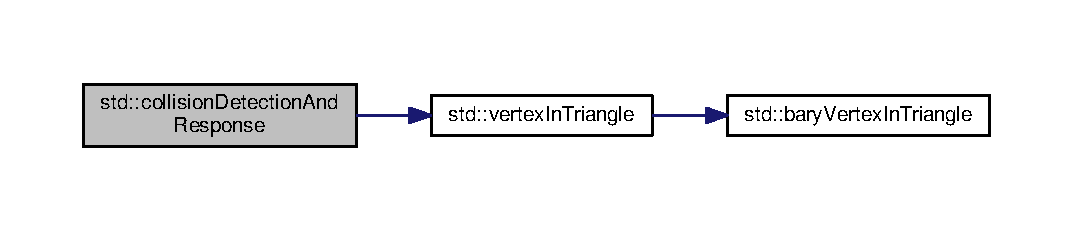
\includegraphics[width=350pt]{namespacestd_a21cb14ca4c41a856be94b8fc9ff59c5a_cgraph}
\end{center}
\end{figure}


\hypertarget{namespacestd_a531c113b5d68b2af865bcc27ae4c8cc4}{}\index{std@{std}!f\+\_\+int@{f\+\_\+int}}
\index{f\+\_\+int@{f\+\_\+int}!std@{std}}
\subsubsection[{f\+\_\+int}]{\setlength{\rightskip}{0pt plus 5cm}Eigen\+::\+Vector3d std\+::f\+\_\+int (
\begin{DoxyParamCaption}
\item[{{\bf Mass} \&}]{pt, }
\item[{vector$<$ {\bf Spring} $>$ \&}]{springs}
\end{DoxyParamCaption}
)}\label{namespacestd_a531c113b5d68b2af865bcc27ae4c8cc4}
Compute internal forces of a point.

This is a subroutine for the forward Euler method. 
\begin{DoxyParams}{Parameters}
{\em pt} & the actual point \\
\hline
{\em springs} & vector of springs \\
\hline
\end{DoxyParams}
\begin{DoxyReturn}{Returns}
sum of forces of all springs connected to point pt 
\end{DoxyReturn}
\hypertarget{namespacestd_a8bde1e030dd347ced2d32f063f983420}{}\index{std@{std}!force@{force}}
\index{force@{force}!std@{std}}
\subsubsection[{force}]{\setlength{\rightskip}{0pt plus 5cm}void std\+::force (
\begin{DoxyParamCaption}
\item[{vector$<$ {\bf Mass} $>$ \&}]{points, }
\item[{vector$<$ {\bf Spring} $>$ \&}]{springs, }
\item[{bool}]{interaction}
\end{DoxyParamCaption}
)}\label{namespacestd_a8bde1e030dd347ced2d32f063f983420}
Calculate force for all points at time t according to x(t) stored in the points.

This is a subroutine for the midpoint method. 
\begin{DoxyParams}{Parameters}
{\em points} & all mass-\/points \\
\hline
{\em springs} & all springs \\
\hline
{\em interaction} & true = apply external forces other than gravity \\
\hline
\end{DoxyParams}


Here is the call graph for this function\+:\nopagebreak
\begin{figure}[H]
\begin{center}
\leavevmode
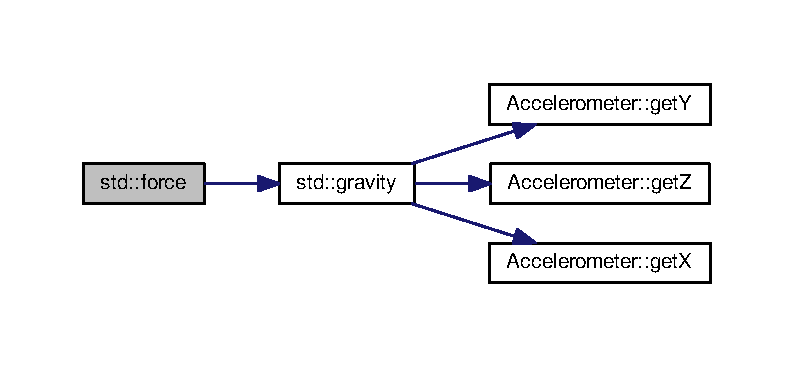
\includegraphics[width=350pt]{namespacestd_a8bde1e030dd347ced2d32f063f983420_cgraph}
\end{center}
\end{figure}


\hypertarget{namespacestd_a799147cff61c9c79a5ef80489d410fe2}{}\index{std@{std}!fwd\+\_\+euler@{fwd\+\_\+euler}}
\index{fwd\+\_\+euler@{fwd\+\_\+euler}!std@{std}}
\subsubsection[{fwd\+\_\+euler}]{\setlength{\rightskip}{0pt plus 5cm}void std\+::fwd\+\_\+euler (
\begin{DoxyParamCaption}
\item[{double}]{dt, }
\item[{vector$<$ {\bf Mass} $>$ \&}]{points, }
\item[{vector$<$ {\bf Spring} $>$ \&}]{springs, }
\item[{bool}]{interaction}
\end{DoxyParamCaption}
)}\label{namespacestd_a799147cff61c9c79a5ef80489d410fe2}
Euler Method -\/ Implementation.

This function calculates the position and velocity for the next time step. 
\begin{DoxyCode}
\textcolor{preprocessor}{# Compute position at t+h      x(t+h) = x(t) + h*v(t)}
\textcolor{preprocessor}{# Compute forces at t          f(t)   = f\_int(t) + f\_ext(t)}
\textcolor{preprocessor}{# Compute acceleration at t    a(t)   = 1/m (f(t) - gamma*v(t))}
\textcolor{preprocessor}{# Compute velocity at t+h      v(t+h) = v(t) + h*a(t)}
\end{DoxyCode}



\begin{DoxyParams}{Parameters}
{\em dt} & time step \\
\hline
{\em points} & all mass-\/points \\
\hline
{\em springs} & all springs \\
\hline
{\em interaction} & true = apply external forces other than gravity \\
\hline
\end{DoxyParams}


Here is the call graph for this function\+:\nopagebreak
\begin{figure}[H]
\begin{center}
\leavevmode
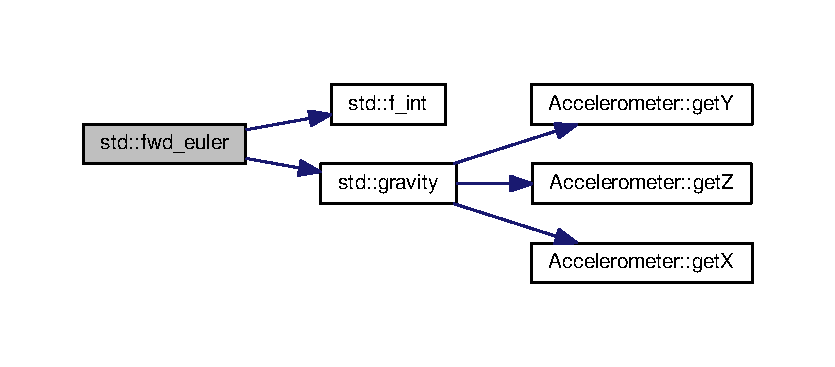
\includegraphics[width=350pt]{namespacestd_a799147cff61c9c79a5ef80489d410fe2_cgraph}
\end{center}
\end{figure}


\hypertarget{namespacestd_a4b332ac1eb524b67a49cfc0187f70b75}{}\index{std@{std}!gravity@{gravity}}
\index{gravity@{gravity}!std@{std}}
\subsubsection[{gravity}]{\setlength{\rightskip}{0pt plus 5cm}Eigen\+::\+Vector3d std\+::gravity (
\begin{DoxyParamCaption}
{}
\end{DoxyParamCaption}
)}\label{namespacestd_a4b332ac1eb524b67a49cfc0187f70b75}
The gravity. Either it is determined from an acceleration sensor or if not detected a constant in Z axis. \begin{DoxyReturn}{Returns}
the gravity 
\end{DoxyReturn}


Here is the call graph for this function\+:\nopagebreak
\begin{figure}[H]
\begin{center}
\leavevmode
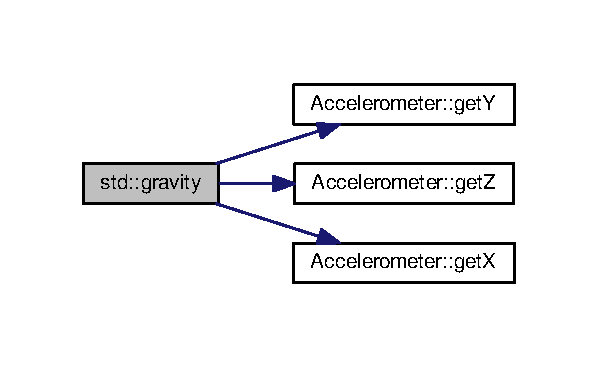
\includegraphics[width=287pt]{namespacestd_a4b332ac1eb524b67a49cfc0187f70b75_cgraph}
\end{center}
\end{figure}


\hypertarget{namespacestd_a6a2a5c73fecc45374baf25b7b05dbc97}{}\index{std@{std}!leapfrog@{leapfrog}}
\index{leapfrog@{leapfrog}!std@{std}}
\subsubsection[{leapfrog}]{\setlength{\rightskip}{0pt plus 5cm}void std\+::leapfrog (
\begin{DoxyParamCaption}
\item[{double}]{dt, }
\item[{vector$<$ {\bf Mass} $>$ \&}]{points, }
\item[{vector$<$ {\bf Spring} $>$ \&}]{springs, }
\item[{bool}]{interaction}
\end{DoxyParamCaption}
)}\label{namespacestd_a6a2a5c73fecc45374baf25b7b05dbc97}
Leapfrog method. 
\begin{DoxyParams}{Parameters}
{\em dt} & time step \\
\hline
{\em points} & all mass-\/points \\
\hline
{\em springs} & all springs \\
\hline
{\em interaction} & true = apply external forces other than gravity \\
\hline
\end{DoxyParams}


Here is the call graph for this function\+:\nopagebreak
\begin{figure}[H]
\begin{center}
\leavevmode
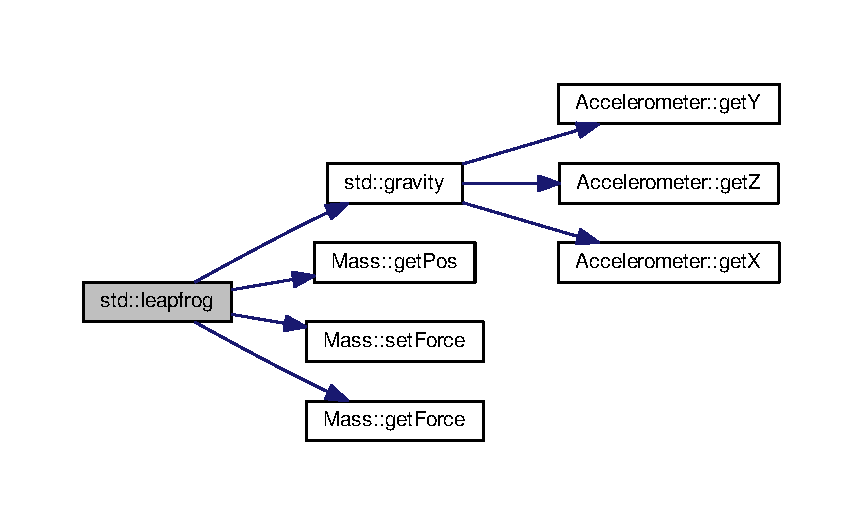
\includegraphics[width=350pt]{namespacestd_a6a2a5c73fecc45374baf25b7b05dbc97_cgraph}
\end{center}
\end{figure}


\hypertarget{namespacestd_ae925c3874f2dd2ec669c4640831d17b6}{}\index{std@{std}!midpoint@{midpoint}}
\index{midpoint@{midpoint}!std@{std}}
\subsubsection[{midpoint}]{\setlength{\rightskip}{0pt plus 5cm}void std\+::midpoint (
\begin{DoxyParamCaption}
\item[{double}]{dt, }
\item[{vector$<$ {\bf Mass} $>$ \&}]{points, }
\item[{vector$<$ {\bf Spring} $>$ \&}]{springs, }
\item[{bool}]{interaction}
\end{DoxyParamCaption}
)}\label{namespacestd_ae925c3874f2dd2ec669c4640831d17b6}
Midpoint method. 
\begin{DoxyCode}
Formula:
  a(\hyperlink{namespacestd_a3546d111a95e4b56d5e75a7ec695a2ee}{t}) = (f(\hyperlink{namespacestd_a3546d111a95e4b56d5e75a7ec695a2ee}{t}) - gamma*v(\hyperlink{namespacestd_a3546d111a95e4b56d5e75a7ec695a2ee}{t}))/m
  v\_half(\hyperlink{namespacestd_a3546d111a95e4b56d5e75a7ec695a2ee}{t}+h/2) = v(\hyperlink{namespacestd_a3546d111a95e4b56d5e75a7ec695a2ee}{t}) + h/2*a(\hyperlink{namespacestd_a3546d111a95e4b56d5e75a7ec695a2ee}{t})
  x\_half(\hyperlink{namespacestd_a3546d111a95e4b56d5e75a7ec695a2ee}{t}+h/2) = x(\hyperlink{namespacestd_a3546d111a95e4b56d5e75a7ec695a2ee}{t}) + h/2*v(\hyperlink{namespacestd_a3546d111a95e4b56d5e75a7ec695a2ee}{t})
  a\_half(\hyperlink{namespacestd_a3546d111a95e4b56d5e75a7ec695a2ee}{t}+h/2) = (f\_half(\hyperlink{namespacestd_a3546d111a95e4b56d5e75a7ec695a2ee}{t}+h/2) - gamma*v\_half(\hyperlink{namespacestd_a3546d111a95e4b56d5e75a7ec695a2ee}{t}+h/2))/m
  x(\hyperlink{namespacestd_a3546d111a95e4b56d5e75a7ec695a2ee}{t}+h) = x(\hyperlink{namespacestd_a3546d111a95e4b56d5e75a7ec695a2ee}{t}) + h*v\_half(\hyperlink{namespacestd_a3546d111a95e4b56d5e75a7ec695a2ee}{t}+h/2)
  v(\hyperlink{namespacestd_a3546d111a95e4b56d5e75a7ec695a2ee}{t}+h) = v(\hyperlink{namespacestd_a3546d111a95e4b56d5e75a7ec695a2ee}{t}) + h*a\_half(\hyperlink{namespacestd_a3546d111a95e4b56d5e75a7ec695a2ee}{t}+h/2)
\end{DoxyCode}



\begin{DoxyParams}{Parameters}
{\em dt} & time step \\
\hline
{\em points} & all mass-\/points \\
\hline
{\em springs} & all springs \\
\hline
{\em interaction} & true = apply external forces other than gravity \\
\hline
\end{DoxyParams}


Here is the call graph for this function\+:\nopagebreak
\begin{figure}[H]
\begin{center}
\leavevmode
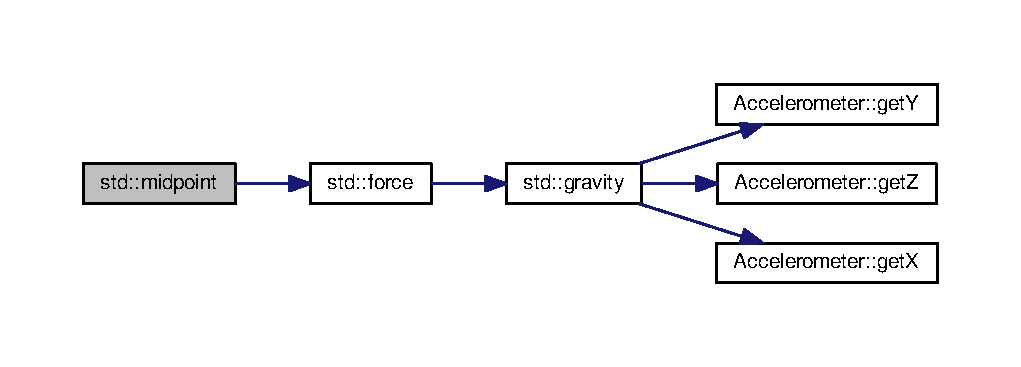
\includegraphics[width=350pt]{namespacestd_ae925c3874f2dd2ec669c4640831d17b6_cgraph}
\end{center}
\end{figure}


\hypertarget{namespacestd_af9b93750ea7aaecab7885d024fd822a2}{}\index{std@{std}!symplectic@{symplectic}}
\index{symplectic@{symplectic}!std@{std}}
\subsubsection[{symplectic}]{\setlength{\rightskip}{0pt plus 5cm}void std\+::symplectic (
\begin{DoxyParamCaption}
\item[{double}]{dt, }
\item[{vector$<$ {\bf Mass} $>$ \&}]{points, }
\item[{vector$<$ {\bf Spring} $>$ \&}]{springs, }
\item[{bool}]{interaction}
\end{DoxyParamCaption}
)}\label{namespacestd_af9b93750ea7aaecab7885d024fd822a2}
Symplectic euler method.


\begin{DoxyCode}
Algorithm:
\textcolor{preprocessor}{# Compute position at t+h      x(t+h) = x(t) + h*v(t)}
\textcolor{preprocessor}{# Compute forces at t          f(t)   = f\_int(t) + f\_ext(t)}
\textcolor{preprocessor}{# Compute acceleration at t    a(t)   = 1/m (f(t) - gamma*v(t))}
\textcolor{preprocessor}{# Compute velocity at t+h      v(t+h) = v(t) + h*a(t)}
\end{DoxyCode}



\begin{DoxyParams}{Parameters}
{\em dt} & time step \\
\hline
{\em points} & all mass-\/points \\
\hline
{\em springs} & all springs \\
\hline
{\em interaction} & true = apply external forces other than gravity \\
\hline
\end{DoxyParams}


Here is the call graph for this function\+:\nopagebreak
\begin{figure}[H]
\begin{center}
\leavevmode
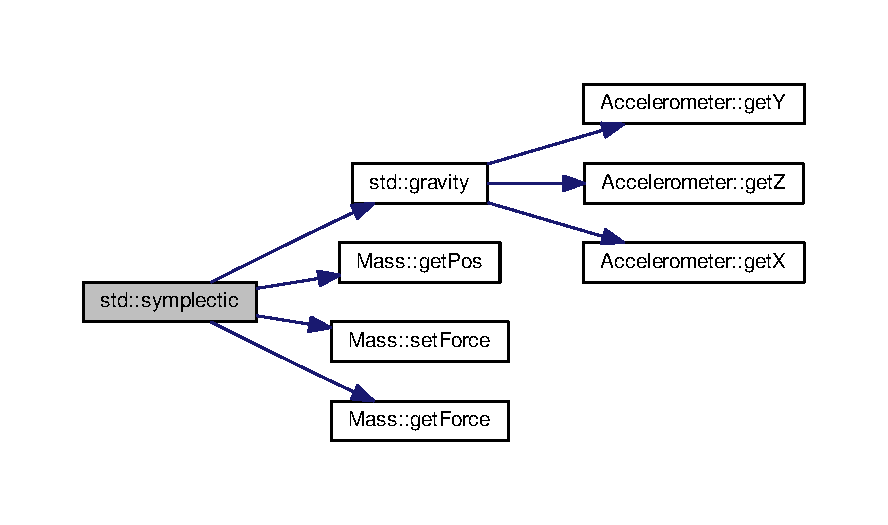
\includegraphics[width=350pt]{namespacestd_af9b93750ea7aaecab7885d024fd822a2_cgraph}
\end{center}
\end{figure}


\hypertarget{namespacestd_a8f17d2dea5f0758f77d130979a6ce6bf}{}\index{std@{std}!vertex\+In\+Triangle@{vertex\+In\+Triangle}}
\index{vertex\+In\+Triangle@{vertex\+In\+Triangle}!std@{std}}
\subsubsection[{vertex\+In\+Triangle}]{\setlength{\rightskip}{0pt plus 5cm}bool std\+::vertex\+In\+Triangle (
\begin{DoxyParamCaption}
\item[{const Eigen\+::\+Vector3d \&}]{P, }
\item[{const Eigen\+::\+Vector3d \&}]{A, }
\item[{const Eigen\+::\+Vector3d \&}]{B, }
\item[{const Eigen\+::\+Vector3d \&}]{C, }
\item[{const float}]{epsilon, }
\item[{float \&}]{dist, }
\item[{Eigen\+::\+Vector3d \&}]{N}
\end{DoxyParamCaption}
)}\label{namespacestd_a8f17d2dea5f0758f77d130979a6ce6bf}


Here is the call graph for this function\+:\nopagebreak
\begin{figure}[H]
\begin{center}
\leavevmode
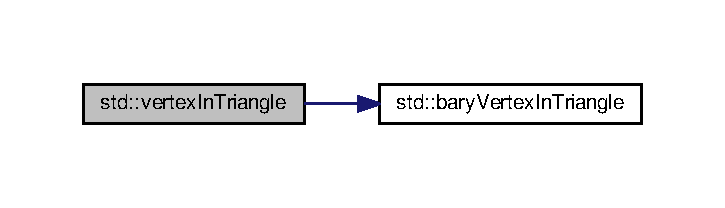
\includegraphics[width=348pt]{namespacestd_a8f17d2dea5f0758f77d130979a6ce6bf_cgraph}
\end{center}
\end{figure}




\subsection{Variable Documentation}
\hypertarget{namespacestd_a3a4f9480c35c84159c4009b499c3eea6}{}\index{std@{std}!floor\+Level@{floor\+Level}}
\index{floor\+Level@{floor\+Level}!std@{std}}
\subsubsection[{floor\+Level}]{\setlength{\rightskip}{0pt plus 5cm}double std\+::floor\+Level = -\/1.}\label{namespacestd_a3a4f9480c35c84159c4009b499c3eea6}
\hypertarget{namespacestd_a46133dbc6d449430af9f3e4b497f0d19}{}\index{std@{std}!leap\+Frog\+Initialized@{leap\+Frog\+Initialized}}
\index{leap\+Frog\+Initialized@{leap\+Frog\+Initialized}!std@{std}}
\subsubsection[{leap\+Frog\+Initialized}]{\setlength{\rightskip}{0pt plus 5cm}bool std\+::leap\+Frog\+Initialized = false}\label{namespacestd_a46133dbc6d449430af9f3e4b497f0d19}
\hypertarget{namespacestd_a339638085d29cb13db371a07634085c6}{}\index{std@{std}!model3d\+Fwd\+Index@{model3d\+Fwd\+Index}}
\index{model3d\+Fwd\+Index@{model3d\+Fwd\+Index}!std@{std}}
\subsubsection[{model3d\+Fwd\+Index}]{\setlength{\rightskip}{0pt plus 5cm}const size\+\_\+t $\ast$$\ast$ std\+::model3d\+Fwd\+Index = {\bf M\+O\+D\+E\+L}(Fwd\+Index)}\label{namespacestd_a339638085d29cb13db371a07634085c6}


indices of the mass-\/points in the positions array 

\hypertarget{namespacestd_a0ff16d332f71a0822fb8570c16df06ff}{}\index{std@{std}!model3d\+Fwd\+Index\+Length@{model3d\+Fwd\+Index\+Length}}
\index{model3d\+Fwd\+Index\+Length@{model3d\+Fwd\+Index\+Length}!std@{std}}
\subsubsection[{model3d\+Fwd\+Index\+Length}]{\setlength{\rightskip}{0pt plus 5cm}const size\+\_\+t $\ast$ std\+::model3d\+Fwd\+Index\+Length = {\bf M\+O\+D\+E\+L}(Fwd\+Index\+Length)}\label{namespacestd_a0ff16d332f71a0822fb8570c16df06ff}


number of indices for each mass-\/point 

\hypertarget{namespacestd_a20a6e87f65453b04a7eac93004989039}{}\index{std@{std}!model3d\+Masses@{model3d\+Masses}}
\index{model3d\+Masses@{model3d\+Masses}!std@{std}}
\subsubsection[{model3d\+Masses}]{\setlength{\rightskip}{0pt plus 5cm}const size\+\_\+t $\ast$ std\+::model3d\+Masses = {\bf M\+O\+D\+E\+L}(Masses)}\label{namespacestd_a20a6e87f65453b04a7eac93004989039}


array of 3\+D-\/objects with mass 

\hypertarget{namespacestd_a22dba9fb8da88b07cd8b471827b6fac7}{}\index{std@{std}!model3d\+Mass\+Fwd\+Offs@{model3d\+Mass\+Fwd\+Offs}}
\index{model3d\+Mass\+Fwd\+Offs@{model3d\+Mass\+Fwd\+Offs}!std@{std}}
\subsubsection[{model3d\+Mass\+Fwd\+Offs}]{\setlength{\rightskip}{0pt plus 5cm}const size\+\_\+t $\ast$ std\+::model3d\+Mass\+Fwd\+Offs = {\bf M\+O\+D\+E\+L}(Mass\+Fwd\+Offs)}\label{namespacestd_a22dba9fb8da88b07cd8b471827b6fac7}


offset in the points array 

\hypertarget{namespacestd_acb567e43ad7c5a09fec7eeed5b529d96}{}\index{std@{std}!model3d\+Mass\+Rev\+Offs@{model3d\+Mass\+Rev\+Offs}}
\index{model3d\+Mass\+Rev\+Offs@{model3d\+Mass\+Rev\+Offs}!std@{std}}
\subsubsection[{model3d\+Mass\+Rev\+Offs}]{\setlength{\rightskip}{0pt plus 5cm}const size\+\_\+t $\ast$ std\+::model3d\+Mass\+Rev\+Offs = {\bf M\+O\+D\+E\+L}(Mass\+Rev\+Offs)}\label{namespacestd_acb567e43ad7c5a09fec7eeed5b529d96}


offsets for the model3d\+Rev\+Index array 

\hypertarget{namespacestd_ad0535524d79ce742b34e78404e55a224}{}\index{std@{std}!model3d\+Mass\+Rev\+Offs\+Orig@{model3d\+Mass\+Rev\+Offs\+Orig}}
\index{model3d\+Mass\+Rev\+Offs\+Orig@{model3d\+Mass\+Rev\+Offs\+Orig}!std@{std}}
\subsubsection[{model3d\+Mass\+Rev\+Offs\+Orig}]{\setlength{\rightskip}{0pt plus 5cm}const size\+\_\+t $\ast$ std\+::model3d\+Mass\+Rev\+Offs\+Orig = {\bf M\+O\+D\+E\+L}(Mass\+Rev\+Offs\+Orig)}\label{namespacestd_ad0535524d79ce742b34e78404e55a224}


offset to the first vertex of an object with mass 

\hypertarget{namespacestd_aea2c80cb8809cdc4c2f3b2b0961d3036}{}\index{std@{std}!model3d\+Mass\+Vertices@{model3d\+Mass\+Vertices}}
\index{model3d\+Mass\+Vertices@{model3d\+Mass\+Vertices}!std@{std}}
\subsubsection[{model3d\+Mass\+Vertices}]{\setlength{\rightskip}{0pt plus 5cm}const size\+\_\+t $\ast$ std\+::model3d\+Mass\+Vertices = {\bf M\+O\+D\+E\+L}(Mass\+Vertices)}\label{namespacestd_aea2c80cb8809cdc4c2f3b2b0961d3036}


number of vertices per object with mass 

\hypertarget{namespacestd_ab62b34140cca60f41eac455edd195e5a}{}\index{std@{std}!model3d\+Normals@{model3d\+Normals}}
\index{model3d\+Normals@{model3d\+Normals}!std@{std}}
\subsubsection[{model3d\+Normals}]{\setlength{\rightskip}{0pt plus 5cm}G\+Lfloat $\ast$ std\+::model3d\+Normals = {\bf M\+O\+D\+E\+L}(Normals)}\label{namespacestd_ab62b34140cca60f41eac455edd195e5a}


all normals of the face surfaces 

\hypertarget{namespacestd_a678ef71cdf9ee666493694bfcf4d238f}{}\index{std@{std}!model3d\+Object\+Length@{model3d\+Object\+Length}}
\index{model3d\+Object\+Length@{model3d\+Object\+Length}!std@{std}}
\subsubsection[{model3d\+Object\+Length}]{\setlength{\rightskip}{0pt plus 5cm}const size\+\_\+t $\ast$ std\+::model3d\+Object\+Length = {\bf M\+O\+D\+E\+L}(Object\+Length)}\label{namespacestd_a678ef71cdf9ee666493694bfcf4d238f}


number of vertices for each 3\+D-\/object 

\hypertarget{namespacestd_af3ac1c474abd23473b8fca32585ffe52}{}\index{std@{std}!model3d\+Object\+Names@{model3d\+Object\+Names}}
\index{model3d\+Object\+Names@{model3d\+Object\+Names}!std@{std}}
\subsubsection[{model3d\+Object\+Names}]{\setlength{\rightskip}{0pt plus 5cm}const char $\ast$$\ast$ std\+::model3d\+Object\+Names = (const char$\ast$$\ast$) {\bf M\+O\+D\+E\+L}(Object\+Names)}\label{namespacestd_af3ac1c474abd23473b8fca32585ffe52}


names of the objects (for identification) 

\hypertarget{namespacestd_a34c26b88877b9e50d420b2f5ee1c1c47}{}\index{std@{std}!model3d\+Object\+Offset@{model3d\+Object\+Offset}}
\index{model3d\+Object\+Offset@{model3d\+Object\+Offset}!std@{std}}
\subsubsection[{model3d\+Object\+Offset}]{\setlength{\rightskip}{0pt plus 5cm}const size\+\_\+t $\ast$ std\+::model3d\+Object\+Offset = {\bf M\+O\+D\+E\+L}(Object\+Offset)}\label{namespacestd_a34c26b88877b9e50d420b2f5ee1c1c47}


offset to the first vertex of a 3\+D-\/object 

\hypertarget{namespacestd_ae8e9077260287353aa87ecaadb67b8e7}{}\index{std@{std}!model3d\+Objects@{model3d\+Objects}}
\index{model3d\+Objects@{model3d\+Objects}!std@{std}}
\subsubsection[{model3d\+Objects}]{\setlength{\rightskip}{0pt plus 5cm}const size\+\_\+t std\+::model3d\+Objects = {\bf M\+O\+D\+E\+L}(Objects)}\label{namespacestd_ae8e9077260287353aa87ecaadb67b8e7}


number of 3\+D-\/objects 

\hypertarget{namespacestd_a74aad4fa6e8a984849221081da2ef691}{}\index{std@{std}!model3d\+Objects\+With\+Mass@{model3d\+Objects\+With\+Mass}}
\index{model3d\+Objects\+With\+Mass@{model3d\+Objects\+With\+Mass}!std@{std}}
\subsubsection[{model3d\+Objects\+With\+Mass}]{\setlength{\rightskip}{0pt plus 5cm}const size\+\_\+t std\+::model3d\+Objects\+With\+Mass = {\bf M\+O\+D\+E\+L}(Objects\+With\+Mass)}\label{namespacestd_a74aad4fa6e8a984849221081da2ef691}


number of objects to apply to the mass-\/spring simulation 

\hypertarget{namespacestd_aa45ed5de4e82f7ca1e4fd453a157715c}{}\index{std@{std}!model3d\+Positions@{model3d\+Positions}}
\index{model3d\+Positions@{model3d\+Positions}!std@{std}}
\subsubsection[{model3d\+Positions}]{\setlength{\rightskip}{0pt plus 5cm}G\+Lfloat $\ast$ std\+::model3d\+Positions = {\bf M\+O\+D\+E\+L}(Positions)}\label{namespacestd_aa45ed5de4e82f7ca1e4fd453a157715c}


all vertex positions 

\hypertarget{namespacestd_a13dd980059224bfd90cd1fde9aa706a9}{}\index{std@{std}!model3d\+Rev\+Index@{model3d\+Rev\+Index}}
\index{model3d\+Rev\+Index@{model3d\+Rev\+Index}!std@{std}}
\subsubsection[{model3d\+Rev\+Index}]{\setlength{\rightskip}{0pt plus 5cm}const size\+\_\+t $\ast$ std\+::model3d\+Rev\+Index = {\bf M\+O\+D\+E\+L}(Rev\+Index)}\label{namespacestd_a13dd980059224bfd90cd1fde9aa706a9}


index of a vertex in the mass-\/points array 

\hypertarget{namespacestd_a75a224804224819d960875bd982ce0c6}{}\index{std@{std}!model3d\+Texels@{model3d\+Texels}}
\index{model3d\+Texels@{model3d\+Texels}!std@{std}}
\subsubsection[{model3d\+Texels}]{\setlength{\rightskip}{0pt plus 5cm}G\+Lfloat $\ast$ std\+::model3d\+Texels = {\bf M\+O\+D\+E\+L}(Texels)}\label{namespacestd_a75a224804224819d960875bd982ce0c6}


all texture coordinates 

\hypertarget{namespacestd_ab193fa08b6666c1bca6ccbb53acd58f6}{}\index{std@{std}!model3d\+Texture\+File\+Path@{model3d\+Texture\+File\+Path}}
\index{model3d\+Texture\+File\+Path@{model3d\+Texture\+File\+Path}!std@{std}}
\subsubsection[{model3d\+Texture\+File\+Path}]{\setlength{\rightskip}{0pt plus 5cm}const char $\ast$ std\+::model3d\+Texture\+File\+Path = \char`\"{}textures/textures\+\_\+all.\+rgb\char`\"{}}\label{namespacestd_ab193fa08b6666c1bca6ccbb53acd58f6}


path to the texture-\/image file 

\hypertarget{namespacestd_a2c56d5934d3e2877598b1eba9302a70f}{}\index{std@{std}!model3d\+Vertices@{model3d\+Vertices}}
\index{model3d\+Vertices@{model3d\+Vertices}!std@{std}}
\subsubsection[{model3d\+Vertices}]{\setlength{\rightskip}{0pt plus 5cm}const size\+\_\+t std\+::model3d\+Vertices = {\bf M\+O\+D\+E\+L}(Vertices)}\label{namespacestd_a2c56d5934d3e2877598b1eba9302a70f}


number of vertices 

\hypertarget{namespacestd_a3901183639dea11eb8cf94025f5cfea8}{}\index{std@{std}!repulsive\+Spring\+Const@{repulsive\+Spring\+Const}}
\index{repulsive\+Spring\+Const@{repulsive\+Spring\+Const}!std@{std}}
\subsubsection[{repulsive\+Spring\+Const}]{\setlength{\rightskip}{0pt plus 5cm}double std\+::repulsive\+Spring\+Const = -\/50.}\label{namespacestd_a3901183639dea11eb8cf94025f5cfea8}
\hypertarget{namespacestd_a3546d111a95e4b56d5e75a7ec695a2ee}{}\index{std@{std}!t@{t}}
\index{t@{t}!std@{std}}
\subsubsection[{t}]{\setlength{\rightskip}{0pt plus 5cm}double std\+::t = 0}\label{namespacestd_a3546d111a95e4b56d5e75a7ec695a2ee}

\chapter{Class Documentation}
\hypertarget{classAccelerometer}{}\section{Accelerometer Class Reference}
\label{classAccelerometer}\index{Accelerometer@{Accelerometer}}


{\ttfamily \#include $<$Accelerometer.\+h$>$}



Collaboration diagram for Accelerometer\+:\nopagebreak
\begin{figure}[H]
\begin{center}
\leavevmode
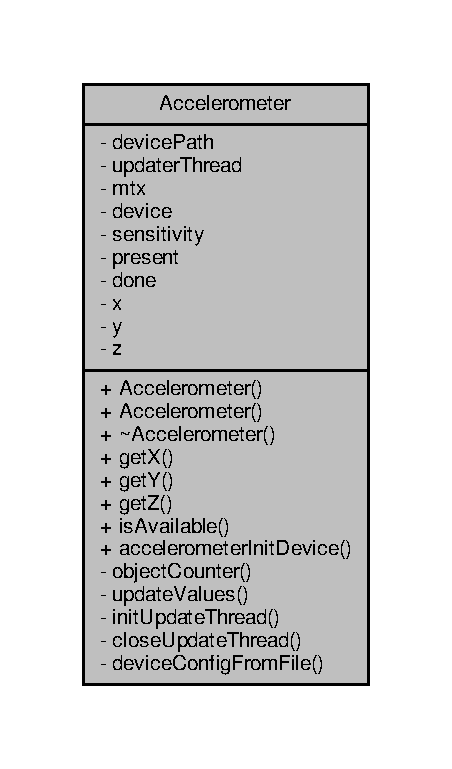
\includegraphics[width=217pt]{classAccelerometer__coll__graph}
\end{center}
\end{figure}
\subsection*{Public Member Functions}
\begin{DoxyCompactItemize}
\item 
\hyperlink{classAccelerometer_aa01d756f8ba70acaaab7938dff643d4d}{Accelerometer} ()
\item 
\hyperlink{classAccelerometer_ac5ae04cdfd2ad1e500fd5cd4c1d10a19}{Accelerometer} (int argc, char $\ast$argv\mbox{[}$\,$\mbox{]})
\item 
\hyperlink{classAccelerometer_acb6a7d9c61f2084ec4aec4a8ff35d622}{$\sim$\+Accelerometer} ()
\item 
double \hyperlink{classAccelerometer_a9c6ac96d56c678b523216b690ff05723}{get\+X} ()
\item 
double \hyperlink{classAccelerometer_ac66896e76f13e8395203a142125f792b}{get\+Y} ()
\item 
double \hyperlink{classAccelerometer_ac35787c41e79c66c25b2c6bde034af87}{get\+Z} ()
\end{DoxyCompactItemize}
\subsection*{Static Public Member Functions}
\begin{DoxyCompactItemize}
\item 
static bool \hyperlink{classAccelerometer_a47ffdc4ab4b99fd0339f964e8a4325f1}{is\+Available} ()
\item 
static void \hyperlink{classAccelerometer_a148aaf7f305b2085c5eacf672007d126}{accelerometer\+Init\+Device} (int argc, char $\ast$argv\mbox{[}$\,$\mbox{]})
\end{DoxyCompactItemize}
\subsection*{Static Private Member Functions}
\begin{DoxyCompactItemize}
\item 
static int \hyperlink{classAccelerometer_ab237ee2d54f41bf5b9cdd1b2d0e30da2}{object\+Counter} (int count)
\item 
static void \hyperlink{classAccelerometer_a0ef1257304190883a415bd1c5d6e2b13}{update\+Values} ()
\item 
static void \hyperlink{classAccelerometer_ae79d97fb2ca83127b10ca309b0732cba}{init\+Update\+Thread} ()
\item 
static void \hyperlink{classAccelerometer_ab8a7687fc06b233e12368b04ec402357}{close\+Update\+Thread} ()
\item 
static void \hyperlink{classAccelerometer_aad6765aee0dbea85d3b5d3fa74a2992c}{device\+Config\+From\+File} (std\+::string config\+Path)
\end{DoxyCompactItemize}
\subsection*{Static Private Attributes}
\begin{DoxyCompactItemize}
\item 
static std\+::string \hyperlink{classAccelerometer_acb0857fa75bff055f25584ae24d362d4}{device\+Path}
\item 
static std\+::thread \hyperlink{classAccelerometer_a8b9d7d942de3ac41f6fe2b2c7e3f15e8}{updater\+Thread}
\item 
static std\+::mutex \hyperlink{classAccelerometer_aa5e00cbce6850be9d3083530bff709dd}{mtx}
\item 
static std\+::ifstream \hyperlink{classAccelerometer_adde7ddf4ba2fae34b4a0910f1a64076b}{device}
\item 
static double \hyperlink{classAccelerometer_a6c600b26e7eeb394058515e8481c8ae0}{sensitivity} = 1.\+0
\item 
static bool \hyperlink{classAccelerometer_a3a11a04b74460eb6ddcf79af3a35e33b}{present} = false
\item 
static bool \hyperlink{classAccelerometer_abe36590009a1913b6886427fc110f531}{done} = false
\item 
static double \hyperlink{classAccelerometer_af06011557497aa4603cbe47966f32aaf}{x} = 0.\+0
\item 
static double \hyperlink{classAccelerometer_a4cba3b73c6339058c046baf1659595fc}{y} = 0.\+0
\item 
static double \hyperlink{classAccelerometer_ac11a92cc27528e883bbfe04cf4a150f7}{z} = 0.\+0
\end{DoxyCompactItemize}


\subsection{Detailed Description}
This class handles the connection to the accelerometer device of a notebook.

Actually it supports the accelerometer of type lis3lv02d. Other devices are unsupported, but they may work with proper settings in the configuration file.~\newline
~\newline
Configuration file\+:~\newline
The file follows the specifications of a windows I\+N\+I file. Here is an example setup\+: 
\begin{DoxyCode}
1 [accelerometer] ; this section must be present
2 device = "/sys/devices/platform/lis3lv02d/position" ; must be an absolute path to the unix device
3 sensitivity = 0.001 ; multiplier to scale the accelerometer output to fit it to gravity force
\end{DoxyCode}
 

\subsection{Constructor \& Destructor Documentation}
\hypertarget{classAccelerometer_aa01d756f8ba70acaaab7938dff643d4d}{}\index{Accelerometer@{Accelerometer}!Accelerometer@{Accelerometer}}
\index{Accelerometer@{Accelerometer}!Accelerometer@{Accelerometer}}
\subsubsection[{Accelerometer}]{\setlength{\rightskip}{0pt plus 5cm}Accelerometer\+::\+Accelerometer (
\begin{DoxyParamCaption}
{}
\end{DoxyParamCaption}
)}\label{classAccelerometer_aa01d756f8ba70acaaab7938dff643d4d}
Construct an accelerometer device handle.

This constructor fails if no device has been initialized previously by using the constructor which takes command line arguments. 

Here is the call graph for this function\+:\nopagebreak
\begin{figure}[H]
\begin{center}
\leavevmode
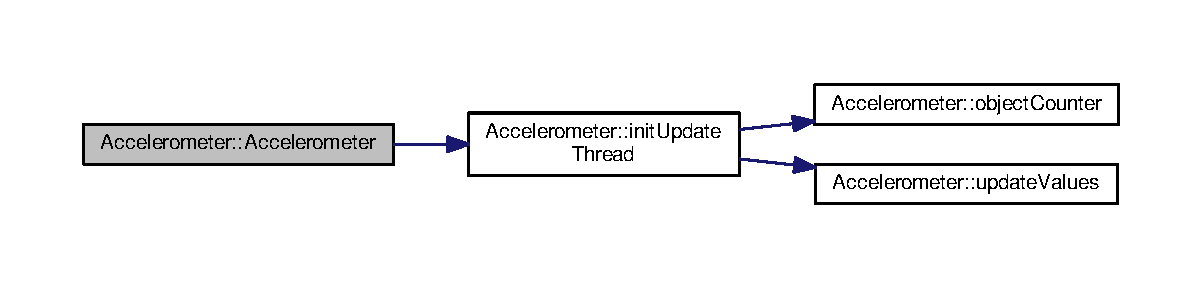
\includegraphics[width=350pt]{classAccelerometer_aa01d756f8ba70acaaab7938dff643d4d_cgraph}
\end{center}
\end{figure}


\hypertarget{classAccelerometer_ac5ae04cdfd2ad1e500fd5cd4c1d10a19}{}\index{Accelerometer@{Accelerometer}!Accelerometer@{Accelerometer}}
\index{Accelerometer@{Accelerometer}!Accelerometer@{Accelerometer}}
\subsubsection[{Accelerometer}]{\setlength{\rightskip}{0pt plus 5cm}Accelerometer\+::\+Accelerometer (
\begin{DoxyParamCaption}
\item[{int}]{argc, }
\item[{char $\ast$}]{argv\mbox{[}$\,$\mbox{]}}
\end{DoxyParamCaption}
)}\label{classAccelerometer_ac5ae04cdfd2ad1e500fd5cd4c1d10a19}
Construct an accelerometer device handle.

This constructor initializes a helping thread which determines periodically data from the device, if it is called the first time. 
\begin{DoxyParams}{Parameters}
{\em argc} & command line arguments counter from {\ttfamily \hyperlink{main_8cpp_a0ddf1224851353fc92bfbff6f499fa97}{main()}} \\
\hline
{\em argv} & arguments vector \\
\hline
\end{DoxyParams}


Here is the call graph for this function\+:\nopagebreak
\begin{figure}[H]
\begin{center}
\leavevmode
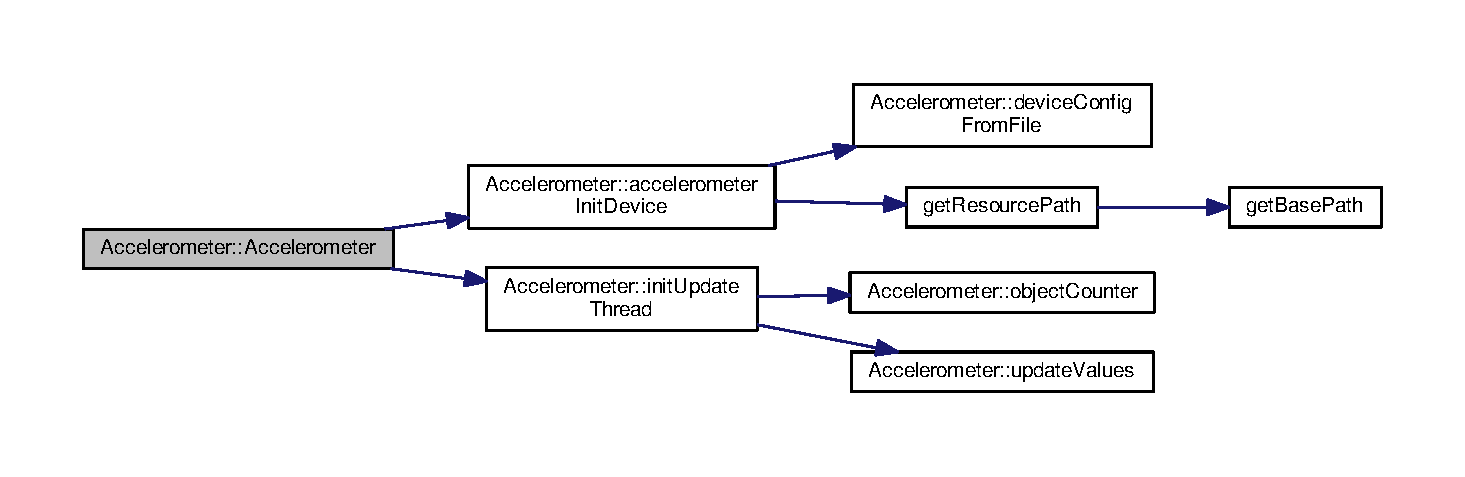
\includegraphics[width=350pt]{classAccelerometer_ac5ae04cdfd2ad1e500fd5cd4c1d10a19_cgraph}
\end{center}
\end{figure}


\hypertarget{classAccelerometer_acb6a7d9c61f2084ec4aec4a8ff35d622}{}\index{Accelerometer@{Accelerometer}!````~Accelerometer@{$\sim$\+Accelerometer}}
\index{````~Accelerometer@{$\sim$\+Accelerometer}!Accelerometer@{Accelerometer}}
\subsubsection[{$\sim$\+Accelerometer}]{\setlength{\rightskip}{0pt plus 5cm}Accelerometer\+::$\sim$\+Accelerometer (
\begin{DoxyParamCaption}
{}
\end{DoxyParamCaption}
)}\label{classAccelerometer_acb6a7d9c61f2084ec4aec4a8ff35d622}
Destroy the device handle.

If the last handle is destroyed, also the connection to the device is closed and the appertaining thread is destroyed. 

Here is the call graph for this function\+:\nopagebreak
\begin{figure}[H]
\begin{center}
\leavevmode
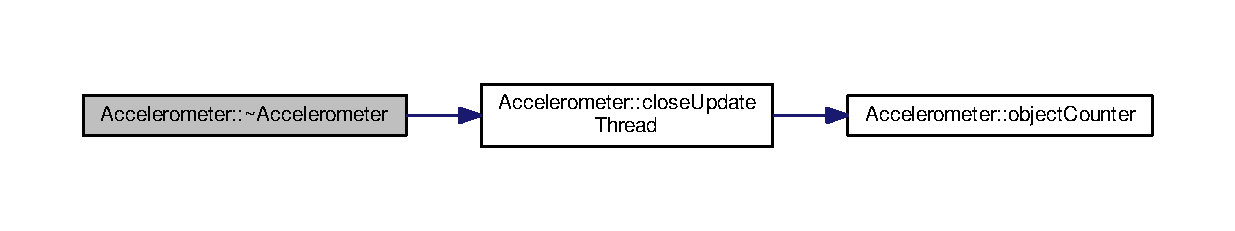
\includegraphics[width=350pt]{classAccelerometer_acb6a7d9c61f2084ec4aec4a8ff35d622_cgraph}
\end{center}
\end{figure}




\subsection{Member Function Documentation}
\hypertarget{classAccelerometer_a148aaf7f305b2085c5eacf672007d126}{}\index{Accelerometer@{Accelerometer}!accelerometer\+Init\+Device@{accelerometer\+Init\+Device}}
\index{accelerometer\+Init\+Device@{accelerometer\+Init\+Device}!Accelerometer@{Accelerometer}}
\subsubsection[{accelerometer\+Init\+Device}]{\setlength{\rightskip}{0pt plus 5cm}void Accelerometer\+::accelerometer\+Init\+Device (
\begin{DoxyParamCaption}
\item[{int}]{argc, }
\item[{char $\ast$}]{argv\mbox{[}$\,$\mbox{]}}
\end{DoxyParamCaption}
)\hspace{0.3cm}{\ttfamily [static]}}\label{classAccelerometer_a148aaf7f305b2085c5eacf672007d126}
Initialize the device.

This method is called by the constructor of the \hyperlink{classAccelerometer}{Accelerometer} class. 
\begin{DoxyParams}{Parameters}
{\em argc} & arguments counter \\
\hline
{\em argv} & arguments vector \\
\hline
\end{DoxyParams}


Here is the call graph for this function\+:\nopagebreak
\begin{figure}[H]
\begin{center}
\leavevmode
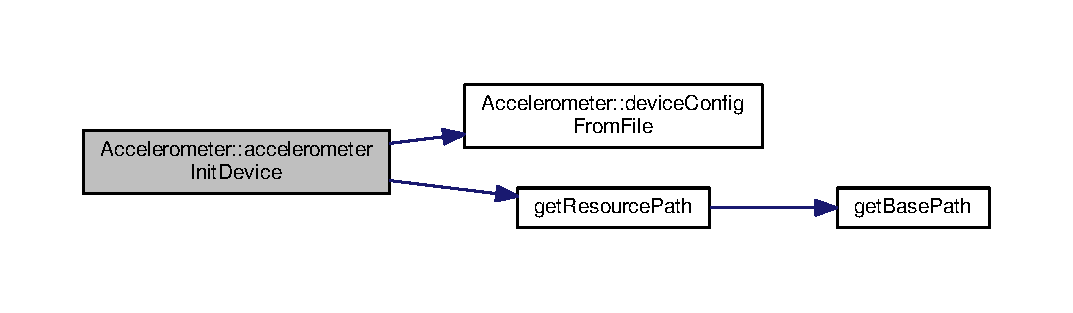
\includegraphics[width=350pt]{classAccelerometer_a148aaf7f305b2085c5eacf672007d126_cgraph}
\end{center}
\end{figure}


\hypertarget{classAccelerometer_ab8a7687fc06b233e12368b04ec402357}{}\index{Accelerometer@{Accelerometer}!close\+Update\+Thread@{close\+Update\+Thread}}
\index{close\+Update\+Thread@{close\+Update\+Thread}!Accelerometer@{Accelerometer}}
\subsubsection[{close\+Update\+Thread}]{\setlength{\rightskip}{0pt plus 5cm}void Accelerometer\+::close\+Update\+Thread (
\begin{DoxyParamCaption}
{}
\end{DoxyParamCaption}
)\hspace{0.3cm}{\ttfamily [static]}, {\ttfamily [private]}}\label{classAccelerometer_ab8a7687fc06b233e12368b04ec402357}
Close the updater thread if the last instance of \hyperlink{classAccelerometer}{Accelerometer} is destroyed. This method is called by the destructor of the \hyperlink{classAccelerometer}{Accelerometer} class. 

Here is the call graph for this function\+:\nopagebreak
\begin{figure}[H]
\begin{center}
\leavevmode
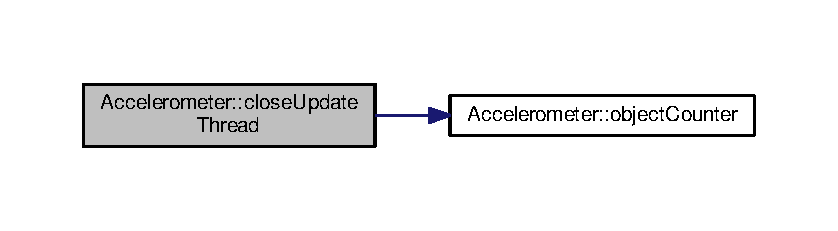
\includegraphics[width=350pt]{classAccelerometer_ab8a7687fc06b233e12368b04ec402357_cgraph}
\end{center}
\end{figure}


\hypertarget{classAccelerometer_aad6765aee0dbea85d3b5d3fa74a2992c}{}\index{Accelerometer@{Accelerometer}!device\+Config\+From\+File@{device\+Config\+From\+File}}
\index{device\+Config\+From\+File@{device\+Config\+From\+File}!Accelerometer@{Accelerometer}}
\subsubsection[{device\+Config\+From\+File}]{\setlength{\rightskip}{0pt plus 5cm}void Accelerometer\+::device\+Config\+From\+File (
\begin{DoxyParamCaption}
\item[{std\+::string}]{config\+Path}
\end{DoxyParamCaption}
)\hspace{0.3cm}{\ttfamily [static]}, {\ttfamily [private]}}\label{classAccelerometer_aad6765aee0dbea85d3b5d3fa74a2992c}
Read configuration for accelerometer device from a config file. 
\begin{DoxyParams}{Parameters}
{\em config\+Path} & path to the config file \\
\hline
\end{DoxyParams}
\hypertarget{classAccelerometer_a9c6ac96d56c678b523216b690ff05723}{}\index{Accelerometer@{Accelerometer}!get\+X@{get\+X}}
\index{get\+X@{get\+X}!Accelerometer@{Accelerometer}}
\subsubsection[{get\+X}]{\setlength{\rightskip}{0pt plus 5cm}double Accelerometer\+::get\+X (
\begin{DoxyParamCaption}
{}
\end{DoxyParamCaption}
)}\label{classAccelerometer_a9c6ac96d56c678b523216b690ff05723}
Get the force into X direction. \begin{DoxyReturn}{Returns}
the force determined from the device. 
\end{DoxyReturn}
\hypertarget{classAccelerometer_ac66896e76f13e8395203a142125f792b}{}\index{Accelerometer@{Accelerometer}!get\+Y@{get\+Y}}
\index{get\+Y@{get\+Y}!Accelerometer@{Accelerometer}}
\subsubsection[{get\+Y}]{\setlength{\rightskip}{0pt plus 5cm}double Accelerometer\+::get\+Y (
\begin{DoxyParamCaption}
{}
\end{DoxyParamCaption}
)}\label{classAccelerometer_ac66896e76f13e8395203a142125f792b}
Get the force into Y direction. \begin{DoxyReturn}{Returns}
the force determined from the device. 
\end{DoxyReturn}
\hypertarget{classAccelerometer_ac35787c41e79c66c25b2c6bde034af87}{}\index{Accelerometer@{Accelerometer}!get\+Z@{get\+Z}}
\index{get\+Z@{get\+Z}!Accelerometer@{Accelerometer}}
\subsubsection[{get\+Z}]{\setlength{\rightskip}{0pt plus 5cm}double Accelerometer\+::get\+Z (
\begin{DoxyParamCaption}
{}
\end{DoxyParamCaption}
)}\label{classAccelerometer_ac35787c41e79c66c25b2c6bde034af87}
Get the force into Z direction. \begin{DoxyReturn}{Returns}
the force determined from the device. 
\end{DoxyReturn}
\hypertarget{classAccelerometer_ae79d97fb2ca83127b10ca309b0732cba}{}\index{Accelerometer@{Accelerometer}!init\+Update\+Thread@{init\+Update\+Thread}}
\index{init\+Update\+Thread@{init\+Update\+Thread}!Accelerometer@{Accelerometer}}
\subsubsection[{init\+Update\+Thread}]{\setlength{\rightskip}{0pt plus 5cm}void Accelerometer\+::init\+Update\+Thread (
\begin{DoxyParamCaption}
{}
\end{DoxyParamCaption}
)\hspace{0.3cm}{\ttfamily [static]}, {\ttfamily [private]}}\label{classAccelerometer_ae79d97fb2ca83127b10ca309b0732cba}
Initialize the updater thread, which reads periodically the state of the accelerometer. This method is called each times an \hyperlink{classAccelerometer}{Accelerometer} object is created. 

Here is the call graph for this function\+:\nopagebreak
\begin{figure}[H]
\begin{center}
\leavevmode
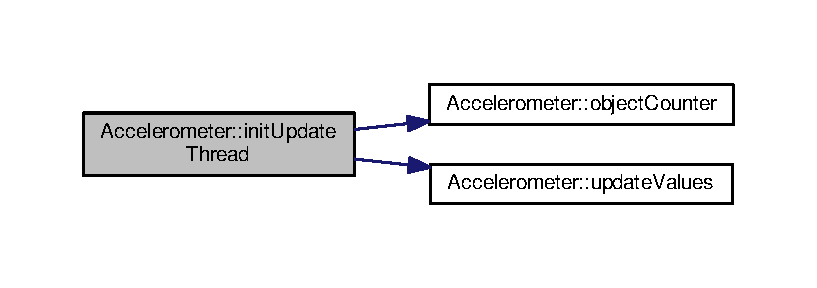
\includegraphics[width=350pt]{classAccelerometer_ae79d97fb2ca83127b10ca309b0732cba_cgraph}
\end{center}
\end{figure}


\hypertarget{classAccelerometer_a47ffdc4ab4b99fd0339f964e8a4325f1}{}\index{Accelerometer@{Accelerometer}!is\+Available@{is\+Available}}
\index{is\+Available@{is\+Available}!Accelerometer@{Accelerometer}}
\subsubsection[{is\+Available}]{\setlength{\rightskip}{0pt plus 5cm}bool Accelerometer\+::is\+Available (
\begin{DoxyParamCaption}
{}
\end{DoxyParamCaption}
)\hspace{0.3cm}{\ttfamily [static]}}\label{classAccelerometer_a47ffdc4ab4b99fd0339f964e8a4325f1}
Checks if the device is present. 
\begin{DoxyRetVals}{Return values}
{\em true} & if the device is online \\
\hline
{\em false} & otherwise \\
\hline
\end{DoxyRetVals}
\hypertarget{classAccelerometer_ab237ee2d54f41bf5b9cdd1b2d0e30da2}{}\index{Accelerometer@{Accelerometer}!object\+Counter@{object\+Counter}}
\index{object\+Counter@{object\+Counter}!Accelerometer@{Accelerometer}}
\subsubsection[{object\+Counter}]{\setlength{\rightskip}{0pt plus 5cm}int Accelerometer\+::object\+Counter (
\begin{DoxyParamCaption}
\item[{int}]{count}
\end{DoxyParamCaption}
)\hspace{0.3cm}{\ttfamily [static]}, {\ttfamily [private]}}\label{classAccelerometer_ab237ee2d54f41bf5b9cdd1b2d0e30da2}
Count the number of open accelerometers 
\begin{DoxyParams}{Parameters}
{\em count} & 1 count up, -\/1 count down or 0 to retrieve without change \\
\hline
\end{DoxyParams}
\begin{DoxyReturn}{Returns}
the counter after change 
\end{DoxyReturn}
\hypertarget{classAccelerometer_a0ef1257304190883a415bd1c5d6e2b13}{}\index{Accelerometer@{Accelerometer}!update\+Values@{update\+Values}}
\index{update\+Values@{update\+Values}!Accelerometer@{Accelerometer}}
\subsubsection[{update\+Values}]{\setlength{\rightskip}{0pt plus 5cm}void Accelerometer\+::update\+Values (
\begin{DoxyParamCaption}
{}
\end{DoxyParamCaption}
)\hspace{0.3cm}{\ttfamily [static]}, {\ttfamily [private]}}\label{classAccelerometer_a0ef1257304190883a415bd1c5d6e2b13}
Updater function delivered to the device-\/handling thread. 

\subsection{Member Data Documentation}
\hypertarget{classAccelerometer_adde7ddf4ba2fae34b4a0910f1a64076b}{}\index{Accelerometer@{Accelerometer}!device@{device}}
\index{device@{device}!Accelerometer@{Accelerometer}}
\subsubsection[{device}]{\setlength{\rightskip}{0pt plus 5cm}std\+::ifstream Accelerometer\+::device\hspace{0.3cm}{\ttfamily [static]}, {\ttfamily [private]}}\label{classAccelerometer_adde7ddf4ba2fae34b4a0910f1a64076b}
\hypertarget{classAccelerometer_acb0857fa75bff055f25584ae24d362d4}{}\index{Accelerometer@{Accelerometer}!device\+Path@{device\+Path}}
\index{device\+Path@{device\+Path}!Accelerometer@{Accelerometer}}
\subsubsection[{device\+Path}]{\setlength{\rightskip}{0pt plus 5cm}std\+::string Accelerometer\+::device\+Path\hspace{0.3cm}{\ttfamily [static]}, {\ttfamily [private]}}\label{classAccelerometer_acb0857fa75bff055f25584ae24d362d4}
\hypertarget{classAccelerometer_abe36590009a1913b6886427fc110f531}{}\index{Accelerometer@{Accelerometer}!done@{done}}
\index{done@{done}!Accelerometer@{Accelerometer}}
\subsubsection[{done}]{\setlength{\rightskip}{0pt plus 5cm}bool Accelerometer\+::done = false\hspace{0.3cm}{\ttfamily [static]}, {\ttfamily [private]}}\label{classAccelerometer_abe36590009a1913b6886427fc110f531}
\hypertarget{classAccelerometer_aa5e00cbce6850be9d3083530bff709dd}{}\index{Accelerometer@{Accelerometer}!mtx@{mtx}}
\index{mtx@{mtx}!Accelerometer@{Accelerometer}}
\subsubsection[{mtx}]{\setlength{\rightskip}{0pt plus 5cm}std\+::mutex Accelerometer\+::mtx\hspace{0.3cm}{\ttfamily [static]}, {\ttfamily [private]}}\label{classAccelerometer_aa5e00cbce6850be9d3083530bff709dd}
\hypertarget{classAccelerometer_a3a11a04b74460eb6ddcf79af3a35e33b}{}\index{Accelerometer@{Accelerometer}!present@{present}}
\index{present@{present}!Accelerometer@{Accelerometer}}
\subsubsection[{present}]{\setlength{\rightskip}{0pt plus 5cm}bool Accelerometer\+::present = false\hspace{0.3cm}{\ttfamily [static]}, {\ttfamily [private]}}\label{classAccelerometer_a3a11a04b74460eb6ddcf79af3a35e33b}
\hypertarget{classAccelerometer_a6c600b26e7eeb394058515e8481c8ae0}{}\index{Accelerometer@{Accelerometer}!sensitivity@{sensitivity}}
\index{sensitivity@{sensitivity}!Accelerometer@{Accelerometer}}
\subsubsection[{sensitivity}]{\setlength{\rightskip}{0pt plus 5cm}double Accelerometer\+::sensitivity = 1.\+0\hspace{0.3cm}{\ttfamily [static]}, {\ttfamily [private]}}\label{classAccelerometer_a6c600b26e7eeb394058515e8481c8ae0}
\hypertarget{classAccelerometer_a8b9d7d942de3ac41f6fe2b2c7e3f15e8}{}\index{Accelerometer@{Accelerometer}!updater\+Thread@{updater\+Thread}}
\index{updater\+Thread@{updater\+Thread}!Accelerometer@{Accelerometer}}
\subsubsection[{updater\+Thread}]{\setlength{\rightskip}{0pt plus 5cm}std\+::thread Accelerometer\+::updater\+Thread\hspace{0.3cm}{\ttfamily [static]}, {\ttfamily [private]}}\label{classAccelerometer_a8b9d7d942de3ac41f6fe2b2c7e3f15e8}
\hypertarget{classAccelerometer_af06011557497aa4603cbe47966f32aaf}{}\index{Accelerometer@{Accelerometer}!x@{x}}
\index{x@{x}!Accelerometer@{Accelerometer}}
\subsubsection[{x}]{\setlength{\rightskip}{0pt plus 5cm}double Accelerometer\+::x = 0.\+0\hspace{0.3cm}{\ttfamily [static]}, {\ttfamily [private]}}\label{classAccelerometer_af06011557497aa4603cbe47966f32aaf}
\hypertarget{classAccelerometer_a4cba3b73c6339058c046baf1659595fc}{}\index{Accelerometer@{Accelerometer}!y@{y}}
\index{y@{y}!Accelerometer@{Accelerometer}}
\subsubsection[{y}]{\setlength{\rightskip}{0pt plus 5cm}double Accelerometer\+::y = 0.\+0\hspace{0.3cm}{\ttfamily [static]}, {\ttfamily [private]}}\label{classAccelerometer_a4cba3b73c6339058c046baf1659595fc}
\hypertarget{classAccelerometer_ac11a92cc27528e883bbfe04cf4a150f7}{}\index{Accelerometer@{Accelerometer}!z@{z}}
\index{z@{z}!Accelerometer@{Accelerometer}}
\subsubsection[{z}]{\setlength{\rightskip}{0pt plus 5cm}double Accelerometer\+::z = 0.\+0\hspace{0.3cm}{\ttfamily [static]}, {\ttfamily [private]}}\label{classAccelerometer_ac11a92cc27528e883bbfe04cf4a150f7}


The documentation for this class was generated from the following files\+:\begin{DoxyCompactItemize}
\item 
src/\hyperlink{Accelerometer_8h}{Accelerometer.\+h}\item 
src/\hyperlink{Accelerometer_8cpp}{Accelerometer.\+cpp}\end{DoxyCompactItemize}

\hypertarget{structImage}{}\section{Image Struct Reference}
\label{structImage}\index{Image@{Image}}


Collaboration diagram for Image\+:\nopagebreak
\begin{figure}[H]
\begin{center}
\leavevmode
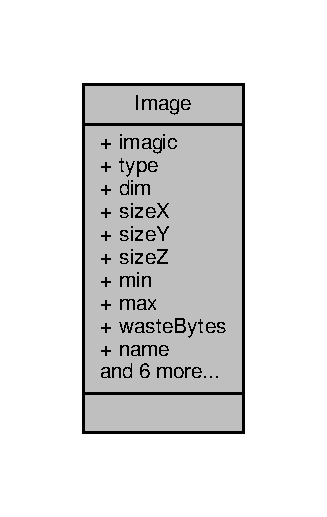
\includegraphics[width=157pt]{structImage__coll__graph}
\end{center}
\end{figure}
\subsection*{Public Attributes}
\begin{DoxyCompactItemize}
\item 
unsigned short \hyperlink{structImage_af799972ef29d6e5f544756ba66f3b6e8}{imagic}
\item 
unsigned short \hyperlink{structImage_a1a32131c2efbb278f0e5f0b554e171b1}{type}
\item 
unsigned short \hyperlink{structImage_a12d84a1935987c4d962564d8419f5eee}{dim}
\item 
unsigned short \hyperlink{structImage_a319a8271c4203b26369f30eca377d4a2}{size\+X}
\item 
unsigned short \hyperlink{structImage_a2559c006462a068477c483c7dbe7cec4}{size\+Y}
\item 
unsigned short \hyperlink{structImage_a260dcb02ec4f3f489245f8d9eb6b4b5f}{size\+Z}
\item 
unsigned int \hyperlink{structImage_a13840d23038045ddd3ced87fc1743eee}{min}
\item 
unsigned int \hyperlink{structImage_ab432fd4170d7b4881d56ec2e0659c033}{max}
\item 
unsigned int \hyperlink{structImage_a767d0814412c848df245e3fd6f4bcc11}{waste\+Bytes}
\item 
char \hyperlink{structImage_a36e3bcd556a3c663614a96c3a7286e11}{name} \mbox{[}80\mbox{]}
\item 
unsigned int \hyperlink{structImage_a6f320ae48d9a3bca2e7f5a6fa501f521}{color\+Map}
\item 
F\+I\+L\+E $\ast$ \hyperlink{structImage_ad4668f1504e7d068753c89cb813d2733}{file}
\item 
unsigned char $\ast$ \hyperlink{structImage_a9baf3bb52b5842bf2ff76ece5a5339a5}{tmp} \mbox{[}5\mbox{]}
\item 
unsigned int \hyperlink{structImage_a5cd308b399153ab7cff993f9fbfa3147}{rle\+End}
\item 
unsigned int $\ast$ \hyperlink{structImage_a8447c2ad0f3d00646c44743bbe7a8b5f}{row\+Start}
\item 
unsigned int $\ast$ \hyperlink{structImage_abf03695b90e13af7e01e9c7ec347d7e0}{row\+Size}
\end{DoxyCompactItemize}


\subsection{Member Data Documentation}
\hypertarget{structImage_a6f320ae48d9a3bca2e7f5a6fa501f521}{}\index{Image@{Image}!color\+Map@{color\+Map}}
\index{color\+Map@{color\+Map}!Image@{Image}}
\subsubsection[{color\+Map}]{\setlength{\rightskip}{0pt plus 5cm}unsigned int Image\+::color\+Map}\label{structImage_a6f320ae48d9a3bca2e7f5a6fa501f521}
\hypertarget{structImage_a12d84a1935987c4d962564d8419f5eee}{}\index{Image@{Image}!dim@{dim}}
\index{dim@{dim}!Image@{Image}}
\subsubsection[{dim}]{\setlength{\rightskip}{0pt plus 5cm}unsigned short Image\+::dim}\label{structImage_a12d84a1935987c4d962564d8419f5eee}
\hypertarget{structImage_ad4668f1504e7d068753c89cb813d2733}{}\index{Image@{Image}!file@{file}}
\index{file@{file}!Image@{Image}}
\subsubsection[{file}]{\setlength{\rightskip}{0pt plus 5cm}F\+I\+L\+E$\ast$ Image\+::file}\label{structImage_ad4668f1504e7d068753c89cb813d2733}
\hypertarget{structImage_af799972ef29d6e5f544756ba66f3b6e8}{}\index{Image@{Image}!imagic@{imagic}}
\index{imagic@{imagic}!Image@{Image}}
\subsubsection[{imagic}]{\setlength{\rightskip}{0pt plus 5cm}unsigned short Image\+::imagic}\label{structImage_af799972ef29d6e5f544756ba66f3b6e8}
\hypertarget{structImage_ab432fd4170d7b4881d56ec2e0659c033}{}\index{Image@{Image}!max@{max}}
\index{max@{max}!Image@{Image}}
\subsubsection[{max}]{\setlength{\rightskip}{0pt plus 5cm}unsigned int Image\+::max}\label{structImage_ab432fd4170d7b4881d56ec2e0659c033}
\hypertarget{structImage_a13840d23038045ddd3ced87fc1743eee}{}\index{Image@{Image}!min@{min}}
\index{min@{min}!Image@{Image}}
\subsubsection[{min}]{\setlength{\rightskip}{0pt plus 5cm}unsigned int Image\+::min}\label{structImage_a13840d23038045ddd3ced87fc1743eee}
\hypertarget{structImage_a36e3bcd556a3c663614a96c3a7286e11}{}\index{Image@{Image}!name@{name}}
\index{name@{name}!Image@{Image}}
\subsubsection[{name}]{\setlength{\rightskip}{0pt plus 5cm}char Image\+::name\mbox{[}80\mbox{]}}\label{structImage_a36e3bcd556a3c663614a96c3a7286e11}
\hypertarget{structImage_a5cd308b399153ab7cff993f9fbfa3147}{}\index{Image@{Image}!rle\+End@{rle\+End}}
\index{rle\+End@{rle\+End}!Image@{Image}}
\subsubsection[{rle\+End}]{\setlength{\rightskip}{0pt plus 5cm}unsigned int Image\+::rle\+End}\label{structImage_a5cd308b399153ab7cff993f9fbfa3147}
\hypertarget{structImage_abf03695b90e13af7e01e9c7ec347d7e0}{}\index{Image@{Image}!row\+Size@{row\+Size}}
\index{row\+Size@{row\+Size}!Image@{Image}}
\subsubsection[{row\+Size}]{\setlength{\rightskip}{0pt plus 5cm}unsigned int$\ast$ Image\+::row\+Size}\label{structImage_abf03695b90e13af7e01e9c7ec347d7e0}
\hypertarget{structImage_a8447c2ad0f3d00646c44743bbe7a8b5f}{}\index{Image@{Image}!row\+Start@{row\+Start}}
\index{row\+Start@{row\+Start}!Image@{Image}}
\subsubsection[{row\+Start}]{\setlength{\rightskip}{0pt plus 5cm}unsigned int$\ast$ Image\+::row\+Start}\label{structImage_a8447c2ad0f3d00646c44743bbe7a8b5f}
\hypertarget{structImage_a319a8271c4203b26369f30eca377d4a2}{}\index{Image@{Image}!size\+X@{size\+X}}
\index{size\+X@{size\+X}!Image@{Image}}
\subsubsection[{size\+X}]{\setlength{\rightskip}{0pt plus 5cm}unsigned short Image\+::size\+X}\label{structImage_a319a8271c4203b26369f30eca377d4a2}
\hypertarget{structImage_a2559c006462a068477c483c7dbe7cec4}{}\index{Image@{Image}!size\+Y@{size\+Y}}
\index{size\+Y@{size\+Y}!Image@{Image}}
\subsubsection[{size\+Y}]{\setlength{\rightskip}{0pt plus 5cm}unsigned short Image\+::size\+Y}\label{structImage_a2559c006462a068477c483c7dbe7cec4}
\hypertarget{structImage_a260dcb02ec4f3f489245f8d9eb6b4b5f}{}\index{Image@{Image}!size\+Z@{size\+Z}}
\index{size\+Z@{size\+Z}!Image@{Image}}
\subsubsection[{size\+Z}]{\setlength{\rightskip}{0pt plus 5cm}unsigned short Image\+::size\+Z}\label{structImage_a260dcb02ec4f3f489245f8d9eb6b4b5f}
\hypertarget{structImage_a9baf3bb52b5842bf2ff76ece5a5339a5}{}\index{Image@{Image}!tmp@{tmp}}
\index{tmp@{tmp}!Image@{Image}}
\subsubsection[{tmp}]{\setlength{\rightskip}{0pt plus 5cm}unsigned char$\ast$ Image\+::tmp\mbox{[}5\mbox{]}}\label{structImage_a9baf3bb52b5842bf2ff76ece5a5339a5}
\hypertarget{structImage_a1a32131c2efbb278f0e5f0b554e171b1}{}\index{Image@{Image}!type@{type}}
\index{type@{type}!Image@{Image}}
\subsubsection[{type}]{\setlength{\rightskip}{0pt plus 5cm}unsigned short Image\+::type}\label{structImage_a1a32131c2efbb278f0e5f0b554e171b1}
\hypertarget{structImage_a767d0814412c848df245e3fd6f4bcc11}{}\index{Image@{Image}!waste\+Bytes@{waste\+Bytes}}
\index{waste\+Bytes@{waste\+Bytes}!Image@{Image}}
\subsubsection[{waste\+Bytes}]{\setlength{\rightskip}{0pt plus 5cm}unsigned int Image\+::waste\+Bytes}\label{structImage_a767d0814412c848df245e3fd6f4bcc11}


The documentation for this struct was generated from the following file\+:\begin{DoxyCompactItemize}
\item 
src/\hyperlink{SGIimage_8c}{S\+G\+Iimage.\+c}\end{DoxyCompactItemize}

\hypertarget{structIMAGE}{}\section{I\+M\+A\+G\+E Struct Reference}
\label{structIMAGE}\index{I\+M\+A\+G\+E@{I\+M\+A\+G\+E}}


{\ttfamily \#include $<$S\+G\+Iimage.\+h$>$}



Collaboration diagram for I\+M\+A\+G\+E\+:\nopagebreak
\begin{figure}[H]
\begin{center}
\leavevmode
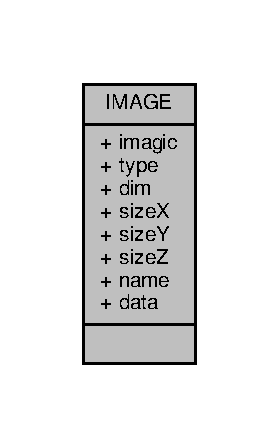
\includegraphics[width=134pt]{structIMAGE__coll__graph}
\end{center}
\end{figure}
\subsection*{Public Attributes}
\begin{DoxyCompactItemize}
\item 
unsigned short \hyperlink{structIMAGE_a29320b057d2ba7f683f5c40e030f9212}{imagic}
\item 
unsigned short \hyperlink{structIMAGE_a310120266ae4398ac530b966b3d43ef0}{type}
\item 
unsigned short \hyperlink{structIMAGE_a18e7e4c0817b235d0cce9d111805e68c}{dim}
\item 
unsigned short \hyperlink{structIMAGE_a9b60e1afa1748197e621d13d6565da24}{size\+X}
\item 
unsigned short \hyperlink{structIMAGE_ab61c98eaf9f32603dfcad280aa90d96b}{size\+Y}
\item 
unsigned short \hyperlink{structIMAGE_ad908fc81625a946abc3eefb3be97a4d5}{size\+Z}
\item 
char \hyperlink{structIMAGE_afc4faf915c6b6cb931fe3631dd29b071}{name} \mbox{[}128\mbox{]}
\item 
unsigned char $\ast$ \hyperlink{structIMAGE_ad2ba44cab5d6a790794d0c37a120453d}{data}
\end{DoxyCompactItemize}


\subsection{Member Data Documentation}
\hypertarget{structIMAGE_ad2ba44cab5d6a790794d0c37a120453d}{}\index{I\+M\+A\+G\+E@{I\+M\+A\+G\+E}!data@{data}}
\index{data@{data}!I\+M\+A\+G\+E@{I\+M\+A\+G\+E}}
\subsubsection[{data}]{\setlength{\rightskip}{0pt plus 5cm}unsigned char$\ast$ I\+M\+A\+G\+E\+::data}\label{structIMAGE_ad2ba44cab5d6a790794d0c37a120453d}
\hypertarget{structIMAGE_a18e7e4c0817b235d0cce9d111805e68c}{}\index{I\+M\+A\+G\+E@{I\+M\+A\+G\+E}!dim@{dim}}
\index{dim@{dim}!I\+M\+A\+G\+E@{I\+M\+A\+G\+E}}
\subsubsection[{dim}]{\setlength{\rightskip}{0pt plus 5cm}unsigned short I\+M\+A\+G\+E\+::dim}\label{structIMAGE_a18e7e4c0817b235d0cce9d111805e68c}
\hypertarget{structIMAGE_a29320b057d2ba7f683f5c40e030f9212}{}\index{I\+M\+A\+G\+E@{I\+M\+A\+G\+E}!imagic@{imagic}}
\index{imagic@{imagic}!I\+M\+A\+G\+E@{I\+M\+A\+G\+E}}
\subsubsection[{imagic}]{\setlength{\rightskip}{0pt plus 5cm}unsigned short I\+M\+A\+G\+E\+::imagic}\label{structIMAGE_a29320b057d2ba7f683f5c40e030f9212}
\hypertarget{structIMAGE_afc4faf915c6b6cb931fe3631dd29b071}{}\index{I\+M\+A\+G\+E@{I\+M\+A\+G\+E}!name@{name}}
\index{name@{name}!I\+M\+A\+G\+E@{I\+M\+A\+G\+E}}
\subsubsection[{name}]{\setlength{\rightskip}{0pt plus 5cm}char I\+M\+A\+G\+E\+::name\mbox{[}128\mbox{]}}\label{structIMAGE_afc4faf915c6b6cb931fe3631dd29b071}
\hypertarget{structIMAGE_a9b60e1afa1748197e621d13d6565da24}{}\index{I\+M\+A\+G\+E@{I\+M\+A\+G\+E}!size\+X@{size\+X}}
\index{size\+X@{size\+X}!I\+M\+A\+G\+E@{I\+M\+A\+G\+E}}
\subsubsection[{size\+X}]{\setlength{\rightskip}{0pt plus 5cm}unsigned short I\+M\+A\+G\+E\+::size\+X}\label{structIMAGE_a9b60e1afa1748197e621d13d6565da24}
\hypertarget{structIMAGE_ab61c98eaf9f32603dfcad280aa90d96b}{}\index{I\+M\+A\+G\+E@{I\+M\+A\+G\+E}!size\+Y@{size\+Y}}
\index{size\+Y@{size\+Y}!I\+M\+A\+G\+E@{I\+M\+A\+G\+E}}
\subsubsection[{size\+Y}]{\setlength{\rightskip}{0pt plus 5cm}unsigned short I\+M\+A\+G\+E\+::size\+Y}\label{structIMAGE_ab61c98eaf9f32603dfcad280aa90d96b}
\hypertarget{structIMAGE_ad908fc81625a946abc3eefb3be97a4d5}{}\index{I\+M\+A\+G\+E@{I\+M\+A\+G\+E}!size\+Z@{size\+Z}}
\index{size\+Z@{size\+Z}!I\+M\+A\+G\+E@{I\+M\+A\+G\+E}}
\subsubsection[{size\+Z}]{\setlength{\rightskip}{0pt plus 5cm}unsigned short I\+M\+A\+G\+E\+::size\+Z}\label{structIMAGE_ad908fc81625a946abc3eefb3be97a4d5}
\hypertarget{structIMAGE_a310120266ae4398ac530b966b3d43ef0}{}\index{I\+M\+A\+G\+E@{I\+M\+A\+G\+E}!type@{type}}
\index{type@{type}!I\+M\+A\+G\+E@{I\+M\+A\+G\+E}}
\subsubsection[{type}]{\setlength{\rightskip}{0pt plus 5cm}unsigned short I\+M\+A\+G\+E\+::type}\label{structIMAGE_a310120266ae4398ac530b966b3d43ef0}


The documentation for this struct was generated from the following file\+:\begin{DoxyCompactItemize}
\item 
src/\hyperlink{SGIimage_8h}{S\+G\+Iimage.\+h}\end{DoxyCompactItemize}

\hypertarget{classMass}{}\section{Mass Class Reference}
\label{classMass}\index{Mass@{Mass}}


{\ttfamily \#include $<$Mass.\+h$>$}



Collaboration diagram for Mass\+:\nopagebreak
\begin{figure}[H]
\begin{center}
\leavevmode
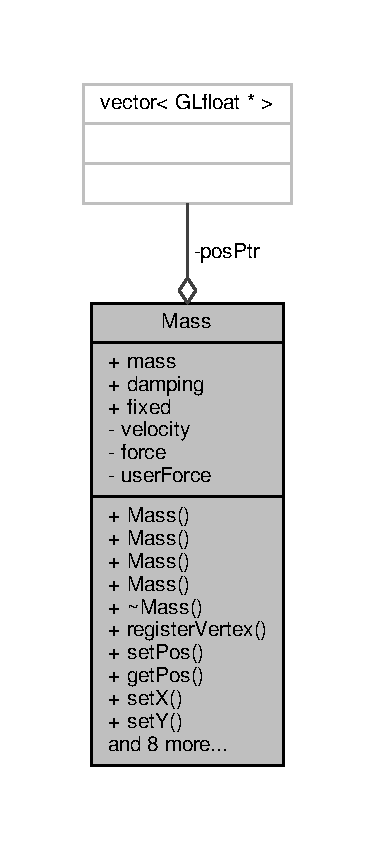
\includegraphics[width=180pt]{classMass__coll__graph}
\end{center}
\end{figure}
\subsection*{Public Member Functions}
\begin{DoxyCompactItemize}
\item 
\hyperlink{classMass_a93c1c52a88d9993644df8b458cacc8ec}{Mass} (std\+::vector$<$ G\+Lfloat $\ast$ $>$ \hyperlink{classMass_abfd5e8aa50988458d702763a48cb438e}{pos\+Ptr}=vector$<$ G\+Lfloat $\ast$ $>$(), double \hyperlink{classMass_a8f37b93ded277000424b7a92adcf9c30}{mass}=0.\+0, double damp=0.\+0)
\item 
\hyperlink{classMass_a4a736155e9f5a484a53705eec56cb282}{Mass} (double \hyperlink{classMass_a8f37b93ded277000424b7a92adcf9c30}{mass}, double damp=0.\+0)
\item 
\hyperlink{classMass_a13584c6157ece49918e644fc2717a7b5}{Mass} (const \hyperlink{classMass}{Mass} \&m)
\item 
\hyperlink{classMass_af1d7e68513a6eb81c1b809583d67fb53}{Mass} (\hyperlink{classMass}{Mass} \&\&)
\item 
virtual \hyperlink{classMass_acbfdfe607e64d1bb2f35ca89900c7136}{$\sim$\+Mass} ()
\item 
void \hyperlink{classMass_acef363ddd9f0f5a42e9d5fe019f5de6c}{register\+Vertex} (G\+Lfloat $\ast$ptr)
\item 
void \hyperlink{classMass_af2b6c3c70c82b277214befdd67c2acbe}{set\+Pos} (Eigen\+::\+Vector3d p)
\item 
Eigen\+::\+Vector3d \hyperlink{classMass_ae07133ef0c5d62612a1126c0e002bd26}{get\+Pos} ()
\item 
void \hyperlink{classMass_a7f1db9674d10a9322f549ee5654a4569}{set\+X} (double x)
\item 
void \hyperlink{classMass_a29e53b261bc6f56cdbd34d458016a627}{set\+Y} (double y)
\item 
void \hyperlink{classMass_adf79327d78c04febb6609bdd1cb4f987}{set\+Z} (double z)
\item 
void \hyperlink{classMass_ac6e500296728680770485a6af1ac4419}{set\+Vel} (Eigen\+::\+Vector3d v)
\item 
Eigen\+::\+Vector3d \hyperlink{classMass_a10e11378951a3dfc97a5029d0b845133}{get\+Vel} ()
\item 
void \hyperlink{classMass_abc2739dab59a65aa3987c91fb010f84c}{set\+Force} (Eigen\+::\+Vector3d f)
\item 
Eigen\+::\+Vector3d \hyperlink{classMass_ab0b0f0e92be4a78dba625cac1e3f8337}{get\+Force} ()
\item 
void \hyperlink{classMass_ad7ec8fa0330bab09feaf536d07aaa1ea}{add\+Force} (Eigen\+::\+Vector3d f)
\item 
void \hyperlink{classMass_ac27a6878abc0caee4ec6af509ef36926}{set\+User\+Force} (Eigen\+::\+Vector3d f)
\item 
Eigen\+::\+Vector3d \hyperlink{classMass_ad295f54d0c63b72db44fc082d27ef1cc}{get\+User\+Force} ()
\end{DoxyCompactItemize}
\subsection*{Public Attributes}
\begin{DoxyCompactItemize}
\item 
double \hyperlink{classMass_a8f37b93ded277000424b7a92adcf9c30}{mass}
\item 
double \hyperlink{classMass_a3b1f3a41fdfc00900a242df309c9c77f}{damping}
\item 
bool \hyperlink{classMass_a596327e28cfa013455a6cd00ca25353e}{fixed}
\end{DoxyCompactItemize}
\subsection*{Private Attributes}
\begin{DoxyCompactItemize}
\item 
vector$<$ G\+Lfloat $\ast$ $>$ \hyperlink{classMass_abfd5e8aa50988458d702763a48cb438e}{pos\+Ptr}
\item 
Eigen\+::\+Vector3d \hyperlink{classMass_ad6fe847559d3f2b4563df4fa3f08f101}{velocity}
\item 
Eigen\+::\+Vector3d \hyperlink{classMass_a5afb4b915d143d4a5156eb7e7e035012}{force}
\item 
Eigen\+::\+Vector3d \hyperlink{classMass_a2e7622d21617bdbf3939ee2ec5784b6d}{user\+Force}
\end{DoxyCompactItemize}


\subsection{Detailed Description}
This class contains all properties of a mass-\/point which are necessary to run a physically based simulation of a mass-\/spring system. 

\subsection{Constructor \& Destructor Documentation}
\hypertarget{classMass_a93c1c52a88d9993644df8b458cacc8ec}{}\index{Mass@{Mass}!Mass@{Mass}}
\index{Mass@{Mass}!Mass@{Mass}}
\subsubsection[{Mass}]{\setlength{\rightskip}{0pt plus 5cm}Mass\+::\+Mass (
\begin{DoxyParamCaption}
\item[{std\+::vector$<$ G\+Lfloat $\ast$ $>$}]{pos\+Ptr = {\ttfamily vector$<$GLfloat$\ast$$>$()}, }
\item[{double}]{mass = {\ttfamily 0.0}, }
\item[{double}]{damp = {\ttfamily 0.0}}
\end{DoxyParamCaption}
)}\label{classMass_a93c1c52a88d9993644df8b458cacc8ec}
Default constructor. 
\begin{DoxyParams}{Parameters}
{\em pos\+Ptr} & vector of pointers to the vertices in the positions array \\
\hline
{\em mass} & the mass of the mass-\/point \\
\hline
{\em damp} & the damping factor of the mass-\/point (to simulate friction and air resistance) \\
\hline
\end{DoxyParams}
\hypertarget{classMass_a4a736155e9f5a484a53705eec56cb282}{}\index{Mass@{Mass}!Mass@{Mass}}
\index{Mass@{Mass}!Mass@{Mass}}
\subsubsection[{Mass}]{\setlength{\rightskip}{0pt plus 5cm}Mass\+::\+Mass (
\begin{DoxyParamCaption}
\item[{double}]{mass, }
\item[{double}]{damp = {\ttfamily 0.0}}
\end{DoxyParamCaption}
)}\label{classMass_a4a736155e9f5a484a53705eec56cb282}
Constructor which takes at least the mass argument. 
\begin{DoxyParams}{Parameters}
{\em mass} & the mass of the mass-\/point \\
\hline
{\em damp} & the damping factor of the mass-\/point (to simulate friction and air resistance) \\
\hline
\end{DoxyParams}
\hypertarget{classMass_a13584c6157ece49918e644fc2717a7b5}{}\index{Mass@{Mass}!Mass@{Mass}}
\index{Mass@{Mass}!Mass@{Mass}}
\subsubsection[{Mass}]{\setlength{\rightskip}{0pt plus 5cm}Mass\+::\+Mass (
\begin{DoxyParamCaption}
\item[{const {\bf Mass} \&}]{m}
\end{DoxyParamCaption}
)}\label{classMass_a13584c6157ece49918e644fc2717a7b5}
Copy constructor 
\begin{DoxyParams}{Parameters}
{\em m} & source object \\
\hline
\end{DoxyParams}
\hypertarget{classMass_af1d7e68513a6eb81c1b809583d67fb53}{}\index{Mass@{Mass}!Mass@{Mass}}
\index{Mass@{Mass}!Mass@{Mass}}
\subsubsection[{Mass}]{\setlength{\rightskip}{0pt plus 5cm}Mass\+::\+Mass (
\begin{DoxyParamCaption}
\item[{{\bf Mass} \&\&}]{m}
\end{DoxyParamCaption}
)}\label{classMass_af1d7e68513a6eb81c1b809583d67fb53}
Move Constructor 
\begin{DoxyParams}{Parameters}
{\em m} & \\
\hline
\end{DoxyParams}
\hypertarget{classMass_acbfdfe607e64d1bb2f35ca89900c7136}{}\index{Mass@{Mass}!````~Mass@{$\sim$\+Mass}}
\index{````~Mass@{$\sim$\+Mass}!Mass@{Mass}}
\subsubsection[{$\sim$\+Mass}]{\setlength{\rightskip}{0pt plus 5cm}Mass\+::$\sim$\+Mass (
\begin{DoxyParamCaption}
{}
\end{DoxyParamCaption}
)\hspace{0.3cm}{\ttfamily [virtual]}}\label{classMass_acbfdfe607e64d1bb2f35ca89900c7136}
Default destructor. 

\subsection{Member Function Documentation}
\hypertarget{classMass_ad7ec8fa0330bab09feaf536d07aaa1ea}{}\index{Mass@{Mass}!add\+Force@{add\+Force}}
\index{add\+Force@{add\+Force}!Mass@{Mass}}
\subsubsection[{add\+Force}]{\setlength{\rightskip}{0pt plus 5cm}void Mass\+::add\+Force (
\begin{DoxyParamCaption}
\item[{Eigen\+::\+Vector3d}]{f}
\end{DoxyParamCaption}
)}\label{classMass_ad7ec8fa0330bab09feaf536d07aaa1ea}
Add a force to the stored value. 
\begin{DoxyParams}{Parameters}
{\em f} & force vector \\
\hline
\end{DoxyParams}
\hypertarget{classMass_ab0b0f0e92be4a78dba625cac1e3f8337}{}\index{Mass@{Mass}!get\+Force@{get\+Force}}
\index{get\+Force@{get\+Force}!Mass@{Mass}}
\subsubsection[{get\+Force}]{\setlength{\rightskip}{0pt plus 5cm}Eigen\+::\+Vector3d Mass\+::get\+Force (
\begin{DoxyParamCaption}
{}
\end{DoxyParamCaption}
)}\label{classMass_ab0b0f0e92be4a78dba625cac1e3f8337}
Get the force. \begin{DoxyReturn}{Returns}
force vector 
\end{DoxyReturn}
\hypertarget{classMass_ae07133ef0c5d62612a1126c0e002bd26}{}\index{Mass@{Mass}!get\+Pos@{get\+Pos}}
\index{get\+Pos@{get\+Pos}!Mass@{Mass}}
\subsubsection[{get\+Pos}]{\setlength{\rightskip}{0pt plus 5cm}Eigen\+::\+Vector3d Mass\+::get\+Pos (
\begin{DoxyParamCaption}
{}
\end{DoxyParamCaption}
)}\label{classMass_ae07133ef0c5d62612a1126c0e002bd26}
Get position vector of mass.

Don\textquotesingle{}t write to the elements of the returned vector. This will lead to inconsistencies in the vertices array. To set a single value use \hyperlink{classMass_a7f1db9674d10a9322f549ee5654a4569}{set\+X()}, \hyperlink{classMass_a29e53b261bc6f56cdbd34d458016a627}{set\+Y()} and \hyperlink{classMass_adf79327d78c04febb6609bdd1cb4f987}{set\+Z()} instead. \begin{DoxyReturn}{Returns}
the position vector or if no vertices are registered the 0 vector. 
\end{DoxyReturn}
\hypertarget{classMass_ad295f54d0c63b72db44fc082d27ef1cc}{}\index{Mass@{Mass}!get\+User\+Force@{get\+User\+Force}}
\index{get\+User\+Force@{get\+User\+Force}!Mass@{Mass}}
\subsubsection[{get\+User\+Force}]{\setlength{\rightskip}{0pt plus 5cm}Eigen\+::\+Vector3d Mass\+::get\+User\+Force (
\begin{DoxyParamCaption}
{}
\end{DoxyParamCaption}
)}\label{classMass_ad295f54d0c63b72db44fc082d27ef1cc}
Get external forces (usually without gravity). \begin{DoxyReturn}{Returns}
force vector 
\end{DoxyReturn}
\hypertarget{classMass_a10e11378951a3dfc97a5029d0b845133}{}\index{Mass@{Mass}!get\+Vel@{get\+Vel}}
\index{get\+Vel@{get\+Vel}!Mass@{Mass}}
\subsubsection[{get\+Vel}]{\setlength{\rightskip}{0pt plus 5cm}Eigen\+::\+Vector3d Mass\+::get\+Vel (
\begin{DoxyParamCaption}
{}
\end{DoxyParamCaption}
)}\label{classMass_a10e11378951a3dfc97a5029d0b845133}
Get the velocity. \begin{DoxyReturn}{Returns}
velocity vector 
\end{DoxyReturn}
\hypertarget{classMass_acef363ddd9f0f5a42e9d5fe019f5de6c}{}\index{Mass@{Mass}!register\+Vertex@{register\+Vertex}}
\index{register\+Vertex@{register\+Vertex}!Mass@{Mass}}
\subsubsection[{register\+Vertex}]{\setlength{\rightskip}{0pt plus 5cm}void Mass\+::register\+Vertex (
\begin{DoxyParamCaption}
\item[{G\+Lfloat $\ast$}]{ptr}
\end{DoxyParamCaption}
)}\label{classMass_acef363ddd9f0f5a42e9d5fe019f5de6c}
Register the pointer to a vertex as position. 
\begin{DoxyParams}{Parameters}
{\em ptr} & pointer targeting the x-\/coordinate of the vertex position. The y-\/ and z-\/coordinates must be in consecutive order in the array. \\
\hline
\end{DoxyParams}
\hypertarget{classMass_abc2739dab59a65aa3987c91fb010f84c}{}\index{Mass@{Mass}!set\+Force@{set\+Force}}
\index{set\+Force@{set\+Force}!Mass@{Mass}}
\subsubsection[{set\+Force}]{\setlength{\rightskip}{0pt plus 5cm}void Mass\+::set\+Force (
\begin{DoxyParamCaption}
\item[{Eigen\+::\+Vector3d}]{f}
\end{DoxyParamCaption}
)}\label{classMass_abc2739dab59a65aa3987c91fb010f84c}
Set the force.

This vector is reserved for the solver. Use {\ttfamily \hyperlink{classMass_ac27a6878abc0caee4ec6af509ef36926}{set\+User\+Force()}} to apply edxternal forces. 
\begin{DoxyParams}{Parameters}
{\em f} & force vector. \\
\hline
\end{DoxyParams}
\hypertarget{classMass_af2b6c3c70c82b277214befdd67c2acbe}{}\index{Mass@{Mass}!set\+Pos@{set\+Pos}}
\index{set\+Pos@{set\+Pos}!Mass@{Mass}}
\subsubsection[{set\+Pos}]{\setlength{\rightskip}{0pt plus 5cm}void Mass\+::set\+Pos (
\begin{DoxyParamCaption}
\item[{Eigen\+::\+Vector3d}]{pos}
\end{DoxyParamCaption}
)}\label{classMass_af2b6c3c70c82b277214befdd67c2acbe}
Set position of the mass object.

This setter spreads the position to all registered vertices. 
\begin{DoxyParams}{Parameters}
{\em pos} & the position vector \\
\hline
\end{DoxyParams}
\hypertarget{classMass_ac27a6878abc0caee4ec6af509ef36926}{}\index{Mass@{Mass}!set\+User\+Force@{set\+User\+Force}}
\index{set\+User\+Force@{set\+User\+Force}!Mass@{Mass}}
\subsubsection[{set\+User\+Force}]{\setlength{\rightskip}{0pt plus 5cm}void Mass\+::set\+User\+Force (
\begin{DoxyParamCaption}
\item[{Eigen\+::\+Vector3d}]{f}
\end{DoxyParamCaption}
)}\label{classMass_ac27a6878abc0caee4ec6af509ef36926}
Set external forces.

Use this setter to apply all external forces except the gravity, the solver applies it separately. 
\begin{DoxyParams}{Parameters}
{\em f} & force vector \\
\hline
\end{DoxyParams}
\hypertarget{classMass_ac6e500296728680770485a6af1ac4419}{}\index{Mass@{Mass}!set\+Vel@{set\+Vel}}
\index{set\+Vel@{set\+Vel}!Mass@{Mass}}
\subsubsection[{set\+Vel}]{\setlength{\rightskip}{0pt plus 5cm}void Mass\+::set\+Vel (
\begin{DoxyParamCaption}
\item[{Eigen\+::\+Vector3d}]{v}
\end{DoxyParamCaption}
)}\label{classMass_ac6e500296728680770485a6af1ac4419}
Set the velocity. 
\begin{DoxyParams}{Parameters}
{\em v} & velocity vector \\
\hline
\end{DoxyParams}
\hypertarget{classMass_a7f1db9674d10a9322f549ee5654a4569}{}\index{Mass@{Mass}!set\+X@{set\+X}}
\index{set\+X@{set\+X}!Mass@{Mass}}
\subsubsection[{set\+X}]{\setlength{\rightskip}{0pt plus 5cm}void Mass\+::set\+X (
\begin{DoxyParamCaption}
\item[{double}]{x}
\end{DoxyParamCaption}
)}\label{classMass_a7f1db9674d10a9322f549ee5654a4569}
Set x-\/coordinate of the mass object.

This setter spreads the x-\/coordinate to all registered vertices. Don\textquotesingle{}t use get\+Pos.\+x to write a coordinate, it will mess up the vertices array. 
\begin{DoxyParams}{Parameters}
{\em x} & the coordinate \\
\hline
\end{DoxyParams}
\hypertarget{classMass_a29e53b261bc6f56cdbd34d458016a627}{}\index{Mass@{Mass}!set\+Y@{set\+Y}}
\index{set\+Y@{set\+Y}!Mass@{Mass}}
\subsubsection[{set\+Y}]{\setlength{\rightskip}{0pt plus 5cm}void Mass\+::set\+Y (
\begin{DoxyParamCaption}
\item[{double}]{y}
\end{DoxyParamCaption}
)}\label{classMass_a29e53b261bc6f56cdbd34d458016a627}
Set y-\/coordinate of the mass object.

This setter spreads the y-\/coordinate to all registered vertices. Don\textquotesingle{}t use get\+Pos.\+y to write a coordinate, it will mess up the vertices array. 
\begin{DoxyParams}{Parameters}
{\em y} & the coordinate \\
\hline
\end{DoxyParams}
\hypertarget{classMass_adf79327d78c04febb6609bdd1cb4f987}{}\index{Mass@{Mass}!set\+Z@{set\+Z}}
\index{set\+Z@{set\+Z}!Mass@{Mass}}
\subsubsection[{set\+Z}]{\setlength{\rightskip}{0pt plus 5cm}void Mass\+::set\+Z (
\begin{DoxyParamCaption}
\item[{double}]{z}
\end{DoxyParamCaption}
)}\label{classMass_adf79327d78c04febb6609bdd1cb4f987}
Set z-\/coordinate of the mass object.

This setter spreads the z-\/coordinate to all registered vertices. Don\textquotesingle{}t use get\+Pos.\+z to write a coordinate, it will mess up the vertices array. 
\begin{DoxyParams}{Parameters}
{\em z} & the coordinate \\
\hline
\end{DoxyParams}


\subsection{Member Data Documentation}
\hypertarget{classMass_a3b1f3a41fdfc00900a242df309c9c77f}{}\index{Mass@{Mass}!damping@{damping}}
\index{damping@{damping}!Mass@{Mass}}
\subsubsection[{damping}]{\setlength{\rightskip}{0pt plus 5cm}double Mass\+::damping}\label{classMass_a3b1f3a41fdfc00900a242df309c9c77f}
\hypertarget{classMass_a596327e28cfa013455a6cd00ca25353e}{}\index{Mass@{Mass}!fixed@{fixed}}
\index{fixed@{fixed}!Mass@{Mass}}
\subsubsection[{fixed}]{\setlength{\rightskip}{0pt plus 5cm}bool Mass\+::fixed}\label{classMass_a596327e28cfa013455a6cd00ca25353e}
\hypertarget{classMass_a5afb4b915d143d4a5156eb7e7e035012}{}\index{Mass@{Mass}!force@{force}}
\index{force@{force}!Mass@{Mass}}
\subsubsection[{force}]{\setlength{\rightskip}{0pt plus 5cm}Eigen\+::\+Vector3d Mass\+::force\hspace{0.3cm}{\ttfamily [private]}}\label{classMass_a5afb4b915d143d4a5156eb7e7e035012}
\hypertarget{classMass_a8f37b93ded277000424b7a92adcf9c30}{}\index{Mass@{Mass}!mass@{mass}}
\index{mass@{mass}!Mass@{Mass}}
\subsubsection[{mass}]{\setlength{\rightskip}{0pt plus 5cm}double Mass\+::mass}\label{classMass_a8f37b93ded277000424b7a92adcf9c30}
\hypertarget{classMass_abfd5e8aa50988458d702763a48cb438e}{}\index{Mass@{Mass}!pos\+Ptr@{pos\+Ptr}}
\index{pos\+Ptr@{pos\+Ptr}!Mass@{Mass}}
\subsubsection[{pos\+Ptr}]{\setlength{\rightskip}{0pt plus 5cm}vector$<$G\+Lfloat$\ast$$>$ Mass\+::pos\+Ptr\hspace{0.3cm}{\ttfamily [private]}}\label{classMass_abfd5e8aa50988458d702763a48cb438e}
\hypertarget{classMass_a2e7622d21617bdbf3939ee2ec5784b6d}{}\index{Mass@{Mass}!user\+Force@{user\+Force}}
\index{user\+Force@{user\+Force}!Mass@{Mass}}
\subsubsection[{user\+Force}]{\setlength{\rightskip}{0pt plus 5cm}Eigen\+::\+Vector3d Mass\+::user\+Force\hspace{0.3cm}{\ttfamily [private]}}\label{classMass_a2e7622d21617bdbf3939ee2ec5784b6d}
\hypertarget{classMass_ad6fe847559d3f2b4563df4fa3f08f101}{}\index{Mass@{Mass}!velocity@{velocity}}
\index{velocity@{velocity}!Mass@{Mass}}
\subsubsection[{velocity}]{\setlength{\rightskip}{0pt plus 5cm}Eigen\+::\+Vector3d Mass\+::velocity\hspace{0.3cm}{\ttfamily [private]}}\label{classMass_ad6fe847559d3f2b4563df4fa3f08f101}


The documentation for this class was generated from the following files\+:\begin{DoxyCompactItemize}
\item 
src/\hyperlink{Mass_8h}{Mass.\+h}\item 
src/\hyperlink{Mass_8cpp}{Mass.\+cpp}\end{DoxyCompactItemize}

\hypertarget{classstd_1_1MipMap}{}\section{std\+:\+:Mip\+Map Class Reference}
\label{classstd_1_1MipMap}\index{std\+::\+Mip\+Map@{std\+::\+Mip\+Map}}


{\ttfamily \#include $<$Mip\+Map.\+h$>$}



Collaboration diagram for std\+:\+:Mip\+Map\+:\nopagebreak
\begin{figure}[H]
\begin{center}
\leavevmode
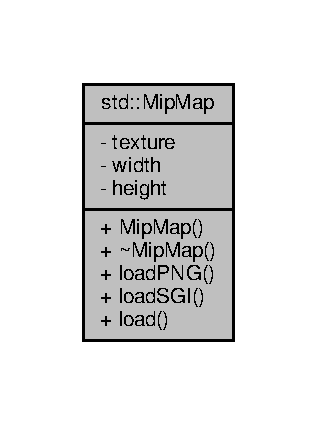
\includegraphics[width=152pt]{classstd_1_1MipMap__coll__graph}
\end{center}
\end{figure}
\subsection*{Public Member Functions}
\begin{DoxyCompactItemize}
\item 
\hyperlink{classstd_1_1MipMap_a2d764943a2f94d50e33c33234966e3f4}{Mip\+Map} ()
\item 
virtual \hyperlink{classstd_1_1MipMap_ac9d8e7ccf0a161b7ae7922ed53abbd6b}{$\sim$\+Mip\+Map} ()
\item 
void \hyperlink{classstd_1_1MipMap_a1b80afd35e90bc8395c33ed2d208f183}{load\+P\+N\+G} (const string file\+Name)
\begin{DoxyCompactList}\small\item\em load texture from P\+N\+G \end{DoxyCompactList}\item 
void \hyperlink{classstd_1_1MipMap_a623e530b676d04b9cd5b07fea6172602}{load\+S\+G\+I} (const string file\+Name)
\begin{DoxyCompactList}\small\item\em load texture from P\+N\+G \end{DoxyCompactList}\item 
void \hyperlink{classstd_1_1MipMap_aa52b162bb516ffe6b7fb5bdc3604ac7d}{load} (const string file\+Name)
\begin{DoxyCompactList}\small\item\em load a texture with a selected import filter \end{DoxyCompactList}\end{DoxyCompactItemize}
\subsection*{Private Attributes}
\begin{DoxyCompactItemize}
\item 
G\+Luint \hyperlink{classstd_1_1MipMap_a9ae62495e98f75e2d545634a0a8b4a61}{texture} = 0
\item 
size\+\_\+t \hyperlink{classstd_1_1MipMap_aa7c7e74f1f05b2d8244f1d06289b18b4}{width} = 0
\item 
size\+\_\+t \hyperlink{classstd_1_1MipMap_a3baac3b8d33da5400b4a4bbca8604436}{height} = 0
\end{DoxyCompactItemize}


\subsection{Detailed Description}
This class is a container for a texture mipmap.

It also handles the loading of an image file.~\newline
Supported file formats\+:~\newline
P\+N\+G images with three colors and no alpha channel S\+G\+I R\+G\+B images with uncompressed data and without alpha channel. 

\subsection{Constructor \& Destructor Documentation}
\hypertarget{classstd_1_1MipMap_a2d764943a2f94d50e33c33234966e3f4}{}\index{std\+::\+Mip\+Map@{std\+::\+Mip\+Map}!Mip\+Map@{Mip\+Map}}
\index{Mip\+Map@{Mip\+Map}!std\+::\+Mip\+Map@{std\+::\+Mip\+Map}}
\subsubsection[{Mip\+Map}]{\setlength{\rightskip}{0pt plus 5cm}std\+::\+Mip\+Map\+::\+Mip\+Map (
\begin{DoxyParamCaption}
{}
\end{DoxyParamCaption}
)}\label{classstd_1_1MipMap_a2d764943a2f94d50e33c33234966e3f4}
Default constructor. \hypertarget{classstd_1_1MipMap_ac9d8e7ccf0a161b7ae7922ed53abbd6b}{}\index{std\+::\+Mip\+Map@{std\+::\+Mip\+Map}!````~Mip\+Map@{$\sim$\+Mip\+Map}}
\index{````~Mip\+Map@{$\sim$\+Mip\+Map}!std\+::\+Mip\+Map@{std\+::\+Mip\+Map}}
\subsubsection[{$\sim$\+Mip\+Map}]{\setlength{\rightskip}{0pt plus 5cm}std\+::\+Mip\+Map\+::$\sim$\+Mip\+Map (
\begin{DoxyParamCaption}
{}
\end{DoxyParamCaption}
)\hspace{0.3cm}{\ttfamily [virtual]}}\label{classstd_1_1MipMap_ac9d8e7ccf0a161b7ae7922ed53abbd6b}
Default destructor. 

\subsection{Member Function Documentation}
\hypertarget{classstd_1_1MipMap_aa52b162bb516ffe6b7fb5bdc3604ac7d}{}\index{std\+::\+Mip\+Map@{std\+::\+Mip\+Map}!load@{load}}
\index{load@{load}!std\+::\+Mip\+Map@{std\+::\+Mip\+Map}}
\subsubsection[{load}]{\setlength{\rightskip}{0pt plus 5cm}void std\+::\+Mip\+Map\+::load (
\begin{DoxyParamCaption}
\item[{const string}]{file\+Name}
\end{DoxyParamCaption}
)}\label{classstd_1_1MipMap_aa52b162bb516ffe6b7fb5bdc3604ac7d}


load a texture with a selected import filter 


\begin{DoxyParams}{Parameters}
{\em file\+Name} & the image file to be loaded \\
\hline
\end{DoxyParams}


Here is the call graph for this function\+:\nopagebreak
\begin{figure}[H]
\begin{center}
\leavevmode
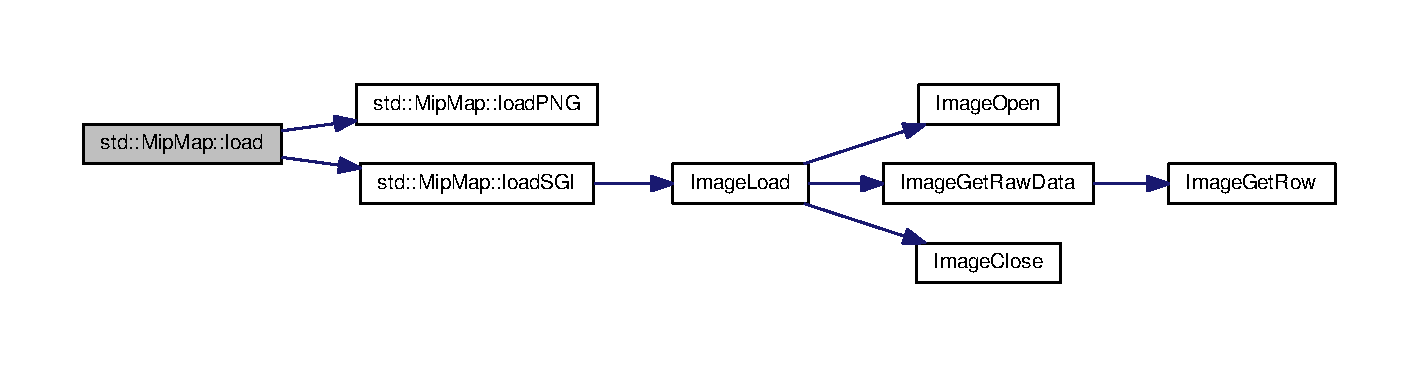
\includegraphics[width=350pt]{classstd_1_1MipMap_aa52b162bb516ffe6b7fb5bdc3604ac7d_cgraph}
\end{center}
\end{figure}


\hypertarget{classstd_1_1MipMap_a1b80afd35e90bc8395c33ed2d208f183}{}\index{std\+::\+Mip\+Map@{std\+::\+Mip\+Map}!load\+P\+N\+G@{load\+P\+N\+G}}
\index{load\+P\+N\+G@{load\+P\+N\+G}!std\+::\+Mip\+Map@{std\+::\+Mip\+Map}}
\subsubsection[{load\+P\+N\+G}]{\setlength{\rightskip}{0pt plus 5cm}void std\+::\+Mip\+Map\+::load\+P\+N\+G (
\begin{DoxyParamCaption}
\item[{const string}]{file\+Name}
\end{DoxyParamCaption}
)}\label{classstd_1_1MipMap_a1b80afd35e90bc8395c33ed2d208f183}


load texture from P\+N\+G 

loads a png file into an opengl mipmap object, using cstdio , libpng, and opengl. This function is almost identical with the example code on \href{https://en.wikibooks.org/wiki/OpenGL_Programming/Intermediate/Textures}{\tt https\+://en.\+wikibooks.\+org/wiki/\+Open\+G\+L\+\_\+\+Programming/\+Intermediate/\+Textures}


\begin{DoxyParams}{Parameters}
{\em file\+Name} & the png file to be loaded \\
\hline
\end{DoxyParams}
\hypertarget{classstd_1_1MipMap_a623e530b676d04b9cd5b07fea6172602}{}\index{std\+::\+Mip\+Map@{std\+::\+Mip\+Map}!load\+S\+G\+I@{load\+S\+G\+I}}
\index{load\+S\+G\+I@{load\+S\+G\+I}!std\+::\+Mip\+Map@{std\+::\+Mip\+Map}}
\subsubsection[{load\+S\+G\+I}]{\setlength{\rightskip}{0pt plus 5cm}void std\+::\+Mip\+Map\+::load\+S\+G\+I (
\begin{DoxyParamCaption}
\item[{const string}]{file\+Name}
\end{DoxyParamCaption}
)}\label{classstd_1_1MipMap_a623e530b676d04b9cd5b07fea6172602}


load texture from P\+N\+G 

loads a R\+G\+B file into an opengl mipmap object, using cstdio , libpng, and opengl. This function is almost identical with the example code on \href{https://en.wikibooks.org/wiki/OpenGL_Programming/Intermediate/Textures}{\tt https\+://en.\+wikibooks.\+org/wiki/\+Open\+G\+L\+\_\+\+Programming/\+Intermediate/\+Textures}


\begin{DoxyParams}{Parameters}
{\em file\+Name} & the S\+G\+I-\/rgb file to be loaded \\
\hline
\end{DoxyParams}


Here is the call graph for this function\+:\nopagebreak
\begin{figure}[H]
\begin{center}
\leavevmode
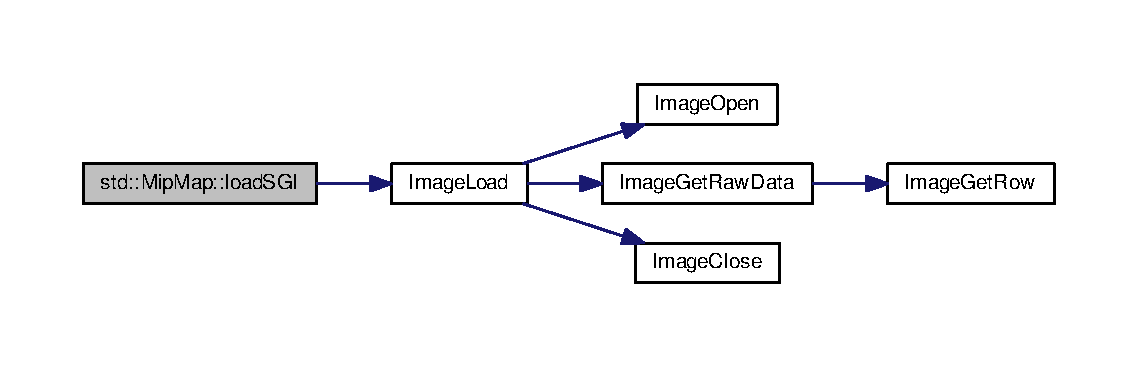
\includegraphics[width=350pt]{classstd_1_1MipMap_a623e530b676d04b9cd5b07fea6172602_cgraph}
\end{center}
\end{figure}




\subsection{Member Data Documentation}
\hypertarget{classstd_1_1MipMap_a3baac3b8d33da5400b4a4bbca8604436}{}\index{std\+::\+Mip\+Map@{std\+::\+Mip\+Map}!height@{height}}
\index{height@{height}!std\+::\+Mip\+Map@{std\+::\+Mip\+Map}}
\subsubsection[{height}]{\setlength{\rightskip}{0pt plus 5cm}size\+\_\+t std\+::\+Mip\+Map\+::height = 0\hspace{0.3cm}{\ttfamily [private]}}\label{classstd_1_1MipMap_a3baac3b8d33da5400b4a4bbca8604436}
\hypertarget{classstd_1_1MipMap_a9ae62495e98f75e2d545634a0a8b4a61}{}\index{std\+::\+Mip\+Map@{std\+::\+Mip\+Map}!texture@{texture}}
\index{texture@{texture}!std\+::\+Mip\+Map@{std\+::\+Mip\+Map}}
\subsubsection[{texture}]{\setlength{\rightskip}{0pt plus 5cm}G\+Luint std\+::\+Mip\+Map\+::texture = 0\hspace{0.3cm}{\ttfamily [private]}}\label{classstd_1_1MipMap_a9ae62495e98f75e2d545634a0a8b4a61}
\hypertarget{classstd_1_1MipMap_aa7c7e74f1f05b2d8244f1d06289b18b4}{}\index{std\+::\+Mip\+Map@{std\+::\+Mip\+Map}!width@{width}}
\index{width@{width}!std\+::\+Mip\+Map@{std\+::\+Mip\+Map}}
\subsubsection[{width}]{\setlength{\rightskip}{0pt plus 5cm}size\+\_\+t std\+::\+Mip\+Map\+::width = 0\hspace{0.3cm}{\ttfamily [private]}}\label{classstd_1_1MipMap_aa7c7e74f1f05b2d8244f1d06289b18b4}


The documentation for this class was generated from the following files\+:\begin{DoxyCompactItemize}
\item 
src/\hyperlink{MipMap_8h}{Mip\+Map.\+h}\item 
src/\hyperlink{MipMap_8cpp}{Mip\+Map.\+cpp}\end{DoxyCompactItemize}

\hypertarget{classstd_1_1Scene}{}\section{std\+:\+:Scene Class Reference}
\label{classstd_1_1Scene}\index{std\+::\+Scene@{std\+::\+Scene}}


{\ttfamily \#include $<$Scene.\+h$>$}



Collaboration diagram for std\+:\+:Scene\+:\nopagebreak
\begin{figure}[H]
\begin{center}
\leavevmode
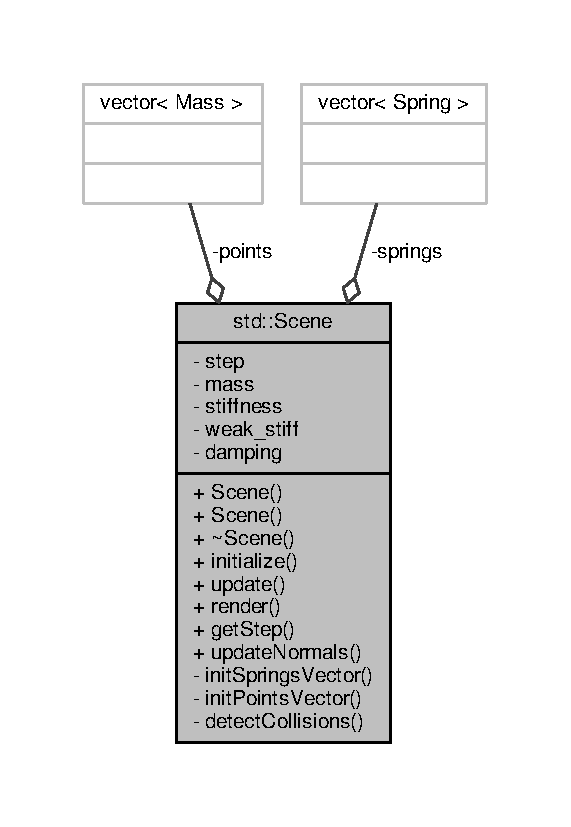
\includegraphics[width=274pt]{classstd_1_1Scene__coll__graph}
\end{center}
\end{figure}
\subsection*{Public Member Functions}
\begin{DoxyCompactItemize}
\item 
\hyperlink{classstd_1_1Scene_a8398f31d8872107aa869418bb7c24c25}{Scene} ()
\item 
\hyperlink{classstd_1_1Scene_ae405abc9a41334e8aadb6e731c44df9c}{Scene} (int argc, char $\ast$argv\mbox{[}$\,$\mbox{]})
\item 
virtual \hyperlink{classstd_1_1Scene_abcd83c86b41e1719e9a140bcf431d881}{$\sim$\+Scene} ()
\item 
void \hyperlink{classstd_1_1Scene_a3e68e24782a8a3d20434b2480ffa46ef}{initialize} ()
\item 
void \hyperlink{classstd_1_1Scene_afe443c3e9196ee13a701a0813e435239}{update} ()
\item 
void \hyperlink{classstd_1_1Scene_a6f5536cb6bf3df944508583badad1bd9}{render} ()
\item 
double \hyperlink{classstd_1_1Scene_a1cb16e4e736e71cd0c7cc53769e24261}{get\+Step} () const 
\item 
void \hyperlink{classstd_1_1Scene_a286eefef820ee9328dce8ec00b15b56f}{update\+Normals} ()
\end{DoxyCompactItemize}
\subsection*{Private Member Functions}
\begin{DoxyCompactItemize}
\item 
void \hyperlink{classstd_1_1Scene_a2616e46d7f209c505d8753f4878dd055}{init\+Springs\+Vector} (size\+\_\+t i)
\item 
void \hyperlink{classstd_1_1Scene_afd32b8076a67538f18533387fc58d61f}{init\+Points\+Vector} (size\+\_\+t i, size\+\_\+t $\ast$n)
\item 
void \hyperlink{classstd_1_1Scene_acf0a57cadc3904cb157058a3f12d8b9a}{detect\+Collisions} ()
\end{DoxyCompactItemize}
\subsection*{Private Attributes}
\begin{DoxyCompactItemize}
\item 
double \hyperlink{classstd_1_1Scene_aba3e53049dcf6b4fb7309a0fe6bb1e2d}{step}
\item 
double \hyperlink{classstd_1_1Scene_a0d5f3e4771f79d5c0f22ef4bd59ca8a7}{mass}
\item 
double \hyperlink{classstd_1_1Scene_af694f3276a68d61649f9fabf2de017d2}{stiffness}
\item 
double \hyperlink{classstd_1_1Scene_a8b5958cd5f7a3f5f03ea8ec6042bceca}{weak\+\_\+stiff}
\item 
double \hyperlink{classstd_1_1Scene_ae8e94f4460f413a412f20a1386f1b308}{damping}
\item 
vector$<$ \hyperlink{classMass}{Mass} $>$ \hyperlink{classstd_1_1Scene_a6666d887df77fc484259f4ad165dcf19}{points}
\item 
vector$<$ \hyperlink{classSpring}{Spring} $>$ \hyperlink{classstd_1_1Scene_a374f417dbcf99c8a314688460876283c}{springs}
\end{DoxyCompactItemize}


\subsection{Detailed Description}
This is a class which handles all tasks to set up, simulate and render a scene with a physical model.

Usually one scene object instance exists program-\/wide. 

\subsection{Constructor \& Destructor Documentation}
\hypertarget{classstd_1_1Scene_a8398f31d8872107aa869418bb7c24c25}{}\index{std\+::\+Scene@{std\+::\+Scene}!Scene@{Scene}}
\index{Scene@{Scene}!std\+::\+Scene@{std\+::\+Scene}}
\subsubsection[{Scene}]{\setlength{\rightskip}{0pt plus 5cm}std\+::\+Scene\+::\+Scene (
\begin{DoxyParamCaption}
{}
\end{DoxyParamCaption}
)}\label{classstd_1_1Scene_a8398f31d8872107aa869418bb7c24c25}
Default constructor \hypertarget{classstd_1_1Scene_ae405abc9a41334e8aadb6e731c44df9c}{}\index{std\+::\+Scene@{std\+::\+Scene}!Scene@{Scene}}
\index{Scene@{Scene}!std\+::\+Scene@{std\+::\+Scene}}
\subsubsection[{Scene}]{\setlength{\rightskip}{0pt plus 5cm}std\+::\+Scene\+::\+Scene (
\begin{DoxyParamCaption}
\item[{int}]{argc, }
\item[{char $\ast$}]{argv\mbox{[}$\,$\mbox{]}}
\end{DoxyParamCaption}
)}\label{classstd_1_1Scene_ae405abc9a41334e8aadb6e731c44df9c}
Constructor which initializes the objectives with values given by command line parameters. 
\begin{DoxyParams}{Parameters}
{\em argc} & arguments counter supplied by the main function \\
\hline
{\em argv} & arguments vector of length {\ttfamily argc} \\
\hline
\end{DoxyParams}
\hypertarget{classstd_1_1Scene_abcd83c86b41e1719e9a140bcf431d881}{}\index{std\+::\+Scene@{std\+::\+Scene}!````~Scene@{$\sim$\+Scene}}
\index{````~Scene@{$\sim$\+Scene}!std\+::\+Scene@{std\+::\+Scene}}
\subsubsection[{$\sim$\+Scene}]{\setlength{\rightskip}{0pt plus 5cm}std\+::\+Scene\+::$\sim$\+Scene (
\begin{DoxyParamCaption}
{}
\end{DoxyParamCaption}
)\hspace{0.3cm}{\ttfamily [virtual]}}\label{classstd_1_1Scene_abcd83c86b41e1719e9a140bcf431d881}
Default destructor. 

\subsection{Member Function Documentation}
\hypertarget{classstd_1_1Scene_acf0a57cadc3904cb157058a3f12d8b9a}{}\index{std\+::\+Scene@{std\+::\+Scene}!detect\+Collisions@{detect\+Collisions}}
\index{detect\+Collisions@{detect\+Collisions}!std\+::\+Scene@{std\+::\+Scene}}
\subsubsection[{detect\+Collisions}]{\setlength{\rightskip}{0pt plus 5cm}void std\+::\+Scene\+::detect\+Collisions (
\begin{DoxyParamCaption}
{}
\end{DoxyParamCaption}
)\hspace{0.3cm}{\ttfamily [private]}}\label{classstd_1_1Scene_acf0a57cadc3904cb157058a3f12d8b9a}
Call the collision detection algorithm for each 3\+D-\/object with mass. 

Here is the call graph for this function\+:\nopagebreak
\begin{figure}[H]
\begin{center}
\leavevmode
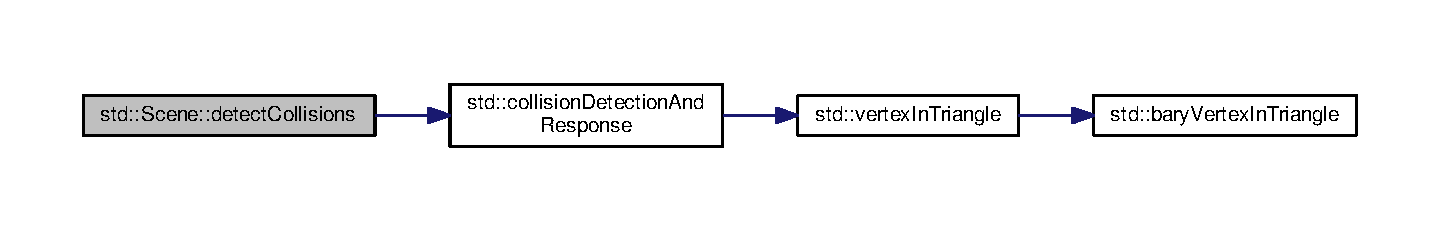
\includegraphics[width=350pt]{classstd_1_1Scene_acf0a57cadc3904cb157058a3f12d8b9a_cgraph}
\end{center}
\end{figure}


\hypertarget{classstd_1_1Scene_a1cb16e4e736e71cd0c7cc53769e24261}{}\index{std\+::\+Scene@{std\+::\+Scene}!get\+Step@{get\+Step}}
\index{get\+Step@{get\+Step}!std\+::\+Scene@{std\+::\+Scene}}
\subsubsection[{get\+Step}]{\setlength{\rightskip}{0pt plus 5cm}double std\+::\+Scene\+::get\+Step (
\begin{DoxyParamCaption}
{}
\end{DoxyParamCaption}
) const}\label{classstd_1_1Scene_a1cb16e4e736e71cd0c7cc53769e24261}
Get the time step for the simulation. \begin{DoxyReturn}{Returns}
step in seconds 
\end{DoxyReturn}
\hypertarget{classstd_1_1Scene_a3e68e24782a8a3d20434b2480ffa46ef}{}\index{std\+::\+Scene@{std\+::\+Scene}!initialize@{initialize}}
\index{initialize@{initialize}!std\+::\+Scene@{std\+::\+Scene}}
\subsubsection[{initialize}]{\setlength{\rightskip}{0pt plus 5cm}void std\+::\+Scene\+::initialize (
\begin{DoxyParamCaption}
{}
\end{DoxyParamCaption}
)}\label{classstd_1_1Scene_a3e68e24782a8a3d20434b2480ffa46ef}
Initialize the scene for rendering and physical simulation. 

Here is the call graph for this function\+:\nopagebreak
\begin{figure}[H]
\begin{center}
\leavevmode
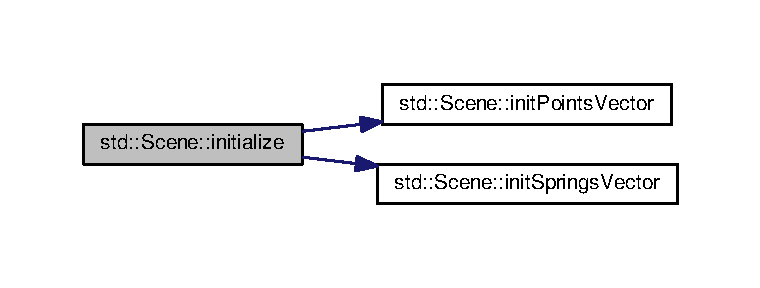
\includegraphics[width=350pt]{classstd_1_1Scene_a3e68e24782a8a3d20434b2480ffa46ef_cgraph}
\end{center}
\end{figure}


\hypertarget{classstd_1_1Scene_afd32b8076a67538f18533387fc58d61f}{}\index{std\+::\+Scene@{std\+::\+Scene}!init\+Points\+Vector@{init\+Points\+Vector}}
\index{init\+Points\+Vector@{init\+Points\+Vector}!std\+::\+Scene@{std\+::\+Scene}}
\subsubsection[{init\+Points\+Vector}]{\setlength{\rightskip}{0pt plus 5cm}void std\+::\+Scene\+::init\+Points\+Vector (
\begin{DoxyParamCaption}
\item[{size\+\_\+t}]{i, }
\item[{size\+\_\+t $\ast$}]{n}
\end{DoxyParamCaption}
)\hspace{0.3cm}{\ttfamily [private]}}\label{classstd_1_1Scene_afd32b8076a67538f18533387fc58d61f}
Initialize all mass-\/points.

This method connects all mass-\/points processed by the physics simulation to the vertices in the ...Positions vector for the renderer. The vector of points must be filled with the correct number of \hyperlink{classMass}{Mass} objects initialized with default values. 
\begin{DoxyParams}{Parameters}
{\em i} & the i-\/th 3d-\/object \\
\hline
{\em n} & a pointer to a counter value, it is incremented with each initialized mass-\/point. it must be initialized with 0 before the first call of this method. \\
\hline
\end{DoxyParams}
\hypertarget{classstd_1_1Scene_a2616e46d7f209c505d8753f4878dd055}{}\index{std\+::\+Scene@{std\+::\+Scene}!init\+Springs\+Vector@{init\+Springs\+Vector}}
\index{init\+Springs\+Vector@{init\+Springs\+Vector}!std\+::\+Scene@{std\+::\+Scene}}
\subsubsection[{init\+Springs\+Vector}]{\setlength{\rightskip}{0pt plus 5cm}void std\+::\+Scene\+::init\+Springs\+Vector (
\begin{DoxyParamCaption}
\item[{size\+\_\+t}]{i}
\end{DoxyParamCaption}
)\hspace{0.3cm}{\ttfamily [private]}}\label{classstd_1_1Scene_a2616e46d7f209c505d8753f4878dd055}
Initialize structural (strong) and bending (weak) springs. No diagonal springs, because of triangular grid


\begin{DoxyParams}{Parameters}
{\em i} & the i-\/th 3\+D-\/object to process \\
\hline
\end{DoxyParams}
\hypertarget{classstd_1_1Scene_a6f5536cb6bf3df944508583badad1bd9}{}\index{std\+::\+Scene@{std\+::\+Scene}!render@{render}}
\index{render@{render}!std\+::\+Scene@{std\+::\+Scene}}
\subsubsection[{render}]{\setlength{\rightskip}{0pt plus 5cm}void std\+::\+Scene\+::render (
\begin{DoxyParamCaption}
{}
\end{DoxyParamCaption}
)}\label{classstd_1_1Scene_a6f5536cb6bf3df944508583badad1bd9}
Render the scene. 

Here is the call graph for this function\+:\nopagebreak
\begin{figure}[H]
\begin{center}
\leavevmode
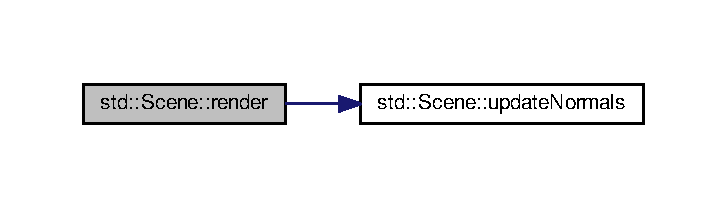
\includegraphics[width=349pt]{classstd_1_1Scene_a6f5536cb6bf3df944508583badad1bd9_cgraph}
\end{center}
\end{figure}


\hypertarget{classstd_1_1Scene_afe443c3e9196ee13a701a0813e435239}{}\index{std\+::\+Scene@{std\+::\+Scene}!update@{update}}
\index{update@{update}!std\+::\+Scene@{std\+::\+Scene}}
\subsubsection[{update}]{\setlength{\rightskip}{0pt plus 5cm}void std\+::\+Scene\+::update (
\begin{DoxyParamCaption}
{}
\end{DoxyParamCaption}
)}\label{classstd_1_1Scene_afe443c3e9196ee13a701a0813e435239}
Update the simulation step and collision detection. 

Here is the call graph for this function\+:\nopagebreak
\begin{figure}[H]
\begin{center}
\leavevmode
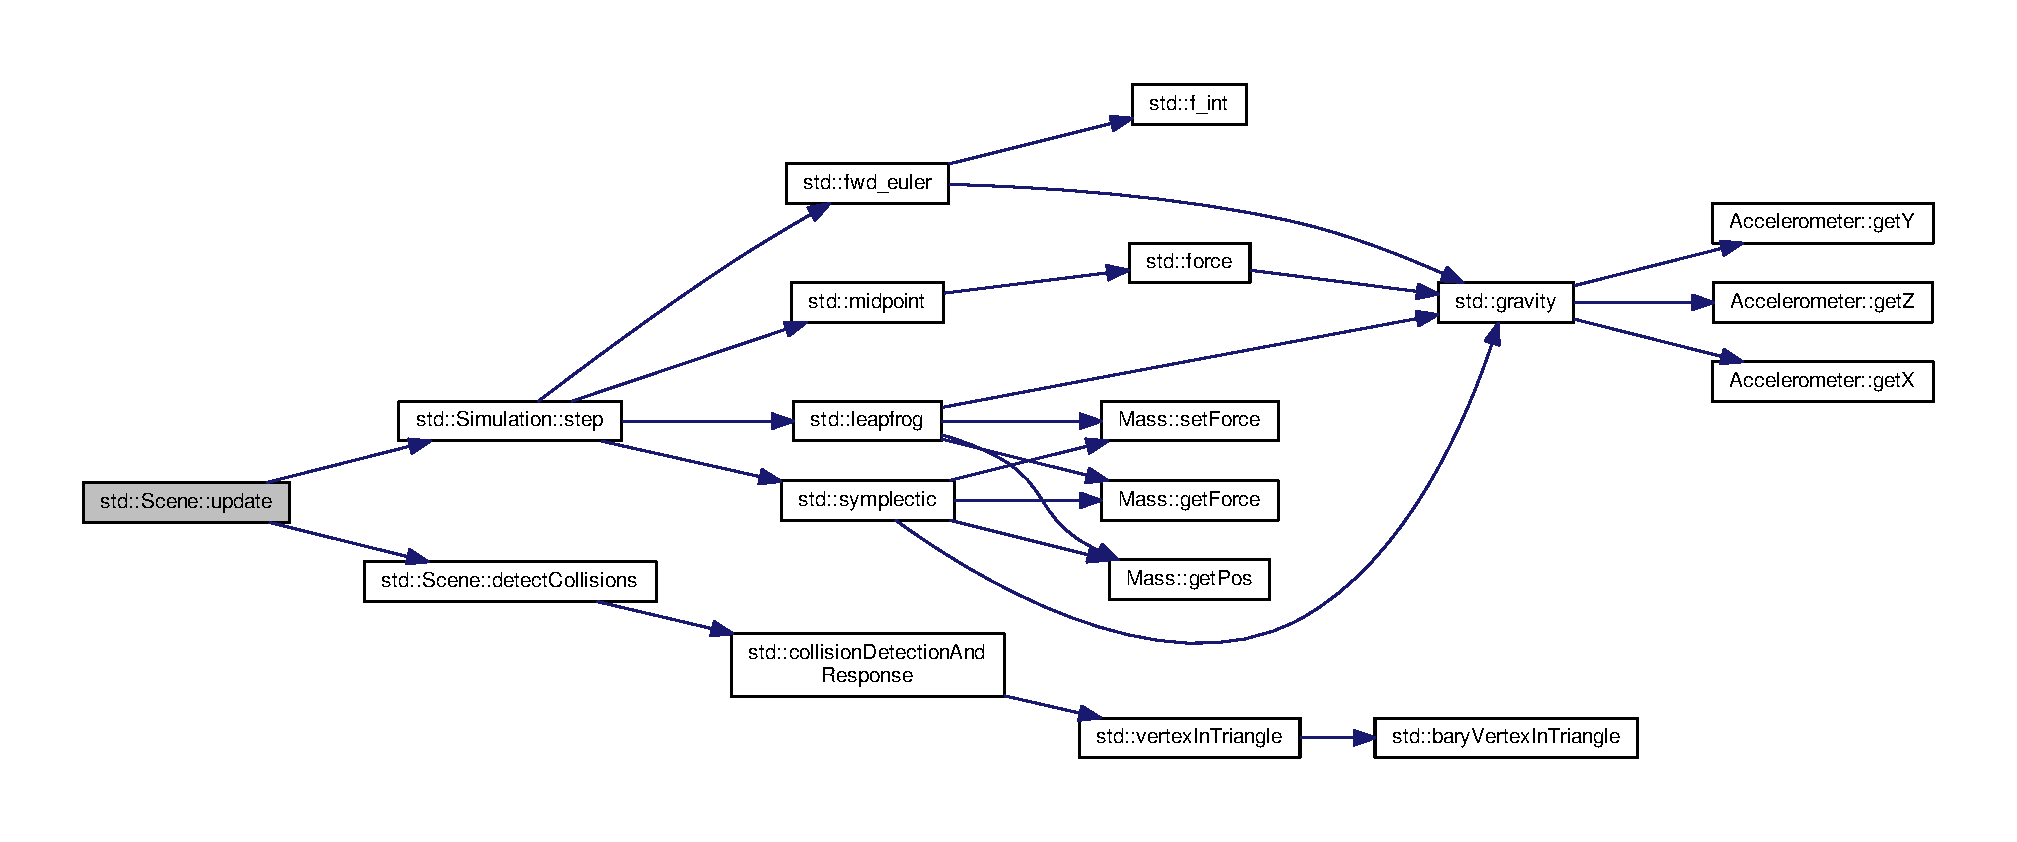
\includegraphics[width=350pt]{classstd_1_1Scene_afe443c3e9196ee13a701a0813e435239_cgraph}
\end{center}
\end{figure}


\hypertarget{classstd_1_1Scene_a286eefef820ee9328dce8ec00b15b56f}{}\index{std\+::\+Scene@{std\+::\+Scene}!update\+Normals@{update\+Normals}}
\index{update\+Normals@{update\+Normals}!std\+::\+Scene@{std\+::\+Scene}}
\subsubsection[{update\+Normals}]{\setlength{\rightskip}{0pt plus 5cm}void std\+::\+Scene\+::update\+Normals (
\begin{DoxyParamCaption}
{}
\end{DoxyParamCaption}
)}\label{classstd_1_1Scene_a286eefef820ee9328dce8ec00b15b56f}
Recalculate all normals for all faces modified by the simulaton step. 

\subsection{Member Data Documentation}
\hypertarget{classstd_1_1Scene_ae8e94f4460f413a412f20a1386f1b308}{}\index{std\+::\+Scene@{std\+::\+Scene}!damping@{damping}}
\index{damping@{damping}!std\+::\+Scene@{std\+::\+Scene}}
\subsubsection[{damping}]{\setlength{\rightskip}{0pt plus 5cm}double std\+::\+Scene\+::damping\hspace{0.3cm}{\ttfamily [private]}}\label{classstd_1_1Scene_ae8e94f4460f413a412f20a1386f1b308}
\hypertarget{classstd_1_1Scene_a0d5f3e4771f79d5c0f22ef4bd59ca8a7}{}\index{std\+::\+Scene@{std\+::\+Scene}!mass@{mass}}
\index{mass@{mass}!std\+::\+Scene@{std\+::\+Scene}}
\subsubsection[{mass}]{\setlength{\rightskip}{0pt plus 5cm}double std\+::\+Scene\+::mass\hspace{0.3cm}{\ttfamily [private]}}\label{classstd_1_1Scene_a0d5f3e4771f79d5c0f22ef4bd59ca8a7}
\hypertarget{classstd_1_1Scene_a6666d887df77fc484259f4ad165dcf19}{}\index{std\+::\+Scene@{std\+::\+Scene}!points@{points}}
\index{points@{points}!std\+::\+Scene@{std\+::\+Scene}}
\subsubsection[{points}]{\setlength{\rightskip}{0pt plus 5cm}vector$<${\bf Mass}$>$ std\+::\+Scene\+::points\hspace{0.3cm}{\ttfamily [private]}}\label{classstd_1_1Scene_a6666d887df77fc484259f4ad165dcf19}
\hypertarget{classstd_1_1Scene_a374f417dbcf99c8a314688460876283c}{}\index{std\+::\+Scene@{std\+::\+Scene}!springs@{springs}}
\index{springs@{springs}!std\+::\+Scene@{std\+::\+Scene}}
\subsubsection[{springs}]{\setlength{\rightskip}{0pt plus 5cm}vector$<${\bf Spring}$>$ std\+::\+Scene\+::springs\hspace{0.3cm}{\ttfamily [private]}}\label{classstd_1_1Scene_a374f417dbcf99c8a314688460876283c}
\hypertarget{classstd_1_1Scene_aba3e53049dcf6b4fb7309a0fe6bb1e2d}{}\index{std\+::\+Scene@{std\+::\+Scene}!step@{step}}
\index{step@{step}!std\+::\+Scene@{std\+::\+Scene}}
\subsubsection[{step}]{\setlength{\rightskip}{0pt plus 5cm}double std\+::\+Scene\+::step\hspace{0.3cm}{\ttfamily [private]}}\label{classstd_1_1Scene_aba3e53049dcf6b4fb7309a0fe6bb1e2d}
\hypertarget{classstd_1_1Scene_af694f3276a68d61649f9fabf2de017d2}{}\index{std\+::\+Scene@{std\+::\+Scene}!stiffness@{stiffness}}
\index{stiffness@{stiffness}!std\+::\+Scene@{std\+::\+Scene}}
\subsubsection[{stiffness}]{\setlength{\rightskip}{0pt plus 5cm}double std\+::\+Scene\+::stiffness\hspace{0.3cm}{\ttfamily [private]}}\label{classstd_1_1Scene_af694f3276a68d61649f9fabf2de017d2}
\hypertarget{classstd_1_1Scene_a8b5958cd5f7a3f5f03ea8ec6042bceca}{}\index{std\+::\+Scene@{std\+::\+Scene}!weak\+\_\+stiff@{weak\+\_\+stiff}}
\index{weak\+\_\+stiff@{weak\+\_\+stiff}!std\+::\+Scene@{std\+::\+Scene}}
\subsubsection[{weak\+\_\+stiff}]{\setlength{\rightskip}{0pt plus 5cm}double std\+::\+Scene\+::weak\+\_\+stiff\hspace{0.3cm}{\ttfamily [private]}}\label{classstd_1_1Scene_a8b5958cd5f7a3f5f03ea8ec6042bceca}


The documentation for this class was generated from the following files\+:\begin{DoxyCompactItemize}
\item 
src/\hyperlink{Scene_8h}{Scene.\+h}\item 
src/\hyperlink{Scene_8cpp}{Scene.\+cpp}\end{DoxyCompactItemize}

\hypertarget{classstd_1_1Simulation}{}\section{std\+:\+:Simulation Class Reference}
\label{classstd_1_1Simulation}\index{std\+::\+Simulation@{std\+::\+Simulation}}


{\ttfamily \#include $<$Simulation.\+h$>$}



Collaboration diagram for std\+:\+:Simulation\+:\nopagebreak
\begin{figure}[H]
\begin{center}
\leavevmode
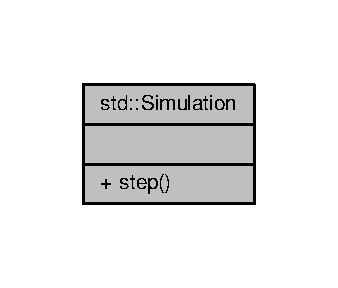
\includegraphics[width=162pt]{classstd_1_1Simulation__coll__graph}
\end{center}
\end{figure}
\subsection*{Public Types}
\begin{DoxyCompactItemize}
\item 
enum \hyperlink{classstd_1_1Simulation_a7cbc16315b54abab3ee481b83d90bf0f}{Method} \{ \hyperlink{classstd_1_1Simulation_a7cbc16315b54abab3ee481b83d90bf0fa21053c5c5a0e88dd4e25f356893b3984}{E\+U\+L\+E\+R}, 
\hyperlink{classstd_1_1Simulation_a7cbc16315b54abab3ee481b83d90bf0fa288a5528e79bb869cfd34673e1182c96}{S\+Y\+M\+P\+L\+E\+C\+T\+I\+C}, 
\hyperlink{classstd_1_1Simulation_a7cbc16315b54abab3ee481b83d90bf0fafe52396efa130f983ce4ab886f04fb49}{L\+E\+A\+P\+F\+R\+O\+G}, 
\hyperlink{classstd_1_1Simulation_a7cbc16315b54abab3ee481b83d90bf0fad2702ad77e7db4ce9edede07636f46db}{M\+I\+D\+P\+O\+I\+N\+T}
 \}
\end{DoxyCompactItemize}
\subsection*{Static Public Member Functions}
\begin{DoxyCompactItemize}
\item 
static void \hyperlink{classstd_1_1Simulation_a0e50b0ce3a31b7ac77cf99b1aa7e3d62}{step} (double dt, \hyperlink{classstd_1_1Simulation_a7cbc16315b54abab3ee481b83d90bf0f}{Method} method, vector$<$ \hyperlink{classMass}{Mass} $>$ \&points, vector$<$ \hyperlink{classSpring}{Spring} $>$ \&springs)
\end{DoxyCompactItemize}


\subsection{Detailed Description}
\hyperlink{classstd_1_1Simulation}{Simulation} class. Solver for mass-\/spring systems.

This class provides some numerical solvers. They are programmed during a assignment of the pro-\/seminar physically based simulations preceding to this project. 

\subsection{Member Enumeration Documentation}
\hypertarget{classstd_1_1Simulation_a7cbc16315b54abab3ee481b83d90bf0f}{}\index{std\+::\+Simulation@{std\+::\+Simulation}!Method@{Method}}
\index{Method@{Method}!std\+::\+Simulation@{std\+::\+Simulation}}
\subsubsection[{Method}]{\setlength{\rightskip}{0pt plus 5cm}enum {\bf std\+::\+Simulation\+::\+Method}}\label{classstd_1_1Simulation_a7cbc16315b54abab3ee481b83d90bf0f}
\begin{Desc}
\item[Enumerator]\par
\begin{description}
\index{E\+U\+L\+E\+R@{E\+U\+L\+E\+R}!std\+::\+Simulation@{std\+::\+Simulation}}\index{std\+::\+Simulation@{std\+::\+Simulation}!E\+U\+L\+E\+R@{E\+U\+L\+E\+R}}\item[{\em 
\hypertarget{classstd_1_1Simulation_a7cbc16315b54abab3ee481b83d90bf0fa21053c5c5a0e88dd4e25f356893b3984}{}E\+U\+L\+E\+R\label{classstd_1_1Simulation_a7cbc16315b54abab3ee481b83d90bf0fa21053c5c5a0e88dd4e25f356893b3984}
}]\index{S\+Y\+M\+P\+L\+E\+C\+T\+I\+C@{S\+Y\+M\+P\+L\+E\+C\+T\+I\+C}!std\+::\+Simulation@{std\+::\+Simulation}}\index{std\+::\+Simulation@{std\+::\+Simulation}!S\+Y\+M\+P\+L\+E\+C\+T\+I\+C@{S\+Y\+M\+P\+L\+E\+C\+T\+I\+C}}\item[{\em 
\hypertarget{classstd_1_1Simulation_a7cbc16315b54abab3ee481b83d90bf0fa288a5528e79bb869cfd34673e1182c96}{}S\+Y\+M\+P\+L\+E\+C\+T\+I\+C\label{classstd_1_1Simulation_a7cbc16315b54abab3ee481b83d90bf0fa288a5528e79bb869cfd34673e1182c96}
}]\index{L\+E\+A\+P\+F\+R\+O\+G@{L\+E\+A\+P\+F\+R\+O\+G}!std\+::\+Simulation@{std\+::\+Simulation}}\index{std\+::\+Simulation@{std\+::\+Simulation}!L\+E\+A\+P\+F\+R\+O\+G@{L\+E\+A\+P\+F\+R\+O\+G}}\item[{\em 
\hypertarget{classstd_1_1Simulation_a7cbc16315b54abab3ee481b83d90bf0fafe52396efa130f983ce4ab886f04fb49}{}L\+E\+A\+P\+F\+R\+O\+G\label{classstd_1_1Simulation_a7cbc16315b54abab3ee481b83d90bf0fafe52396efa130f983ce4ab886f04fb49}
}]\index{M\+I\+D\+P\+O\+I\+N\+T@{M\+I\+D\+P\+O\+I\+N\+T}!std\+::\+Simulation@{std\+::\+Simulation}}\index{std\+::\+Simulation@{std\+::\+Simulation}!M\+I\+D\+P\+O\+I\+N\+T@{M\+I\+D\+P\+O\+I\+N\+T}}\item[{\em 
\hypertarget{classstd_1_1Simulation_a7cbc16315b54abab3ee481b83d90bf0fad2702ad77e7db4ce9edede07636f46db}{}M\+I\+D\+P\+O\+I\+N\+T\label{classstd_1_1Simulation_a7cbc16315b54abab3ee481b83d90bf0fad2702ad77e7db4ce9edede07636f46db}
}]\end{description}
\end{Desc}


\subsection{Member Function Documentation}
\hypertarget{classstd_1_1Simulation_a0e50b0ce3a31b7ac77cf99b1aa7e3d62}{}\index{std\+::\+Simulation@{std\+::\+Simulation}!step@{step}}
\index{step@{step}!std\+::\+Simulation@{std\+::\+Simulation}}
\subsubsection[{step}]{\setlength{\rightskip}{0pt plus 5cm}void std\+::\+Simulation\+::step (
\begin{DoxyParamCaption}
\item[{double}]{dt, }
\item[{{\bf Method}}]{method, }
\item[{vector$<$ {\bf Mass} $>$ \&}]{points, }
\item[{vector$<$ {\bf Spring} $>$ \&}]{springs}
\end{DoxyParamCaption}
)\hspace{0.3cm}{\ttfamily [static]}}\label{classstd_1_1Simulation_a0e50b0ce3a31b7ac77cf99b1aa7e3d62}
Execute one step of the simulation. 
\begin{DoxyParams}{Parameters}
{\em dt} & time delay between two steps \\
\hline
{\em method} & select the method to use; The value can be E\+U\+L\+E\+R, S\+Y\+M\+P\+L\+E\+C\+T\+I\+C, L\+E\+A\+P\+F\+R\+O\+G or M\+I\+D\+P\+O\+I\+N\+T. \\
\hline
{\em points} & all mass-\/points \\
\hline
{\em springs} & all springs \\
\hline
\end{DoxyParams}


Here is the call graph for this function\+:\nopagebreak
\begin{figure}[H]
\begin{center}
\leavevmode
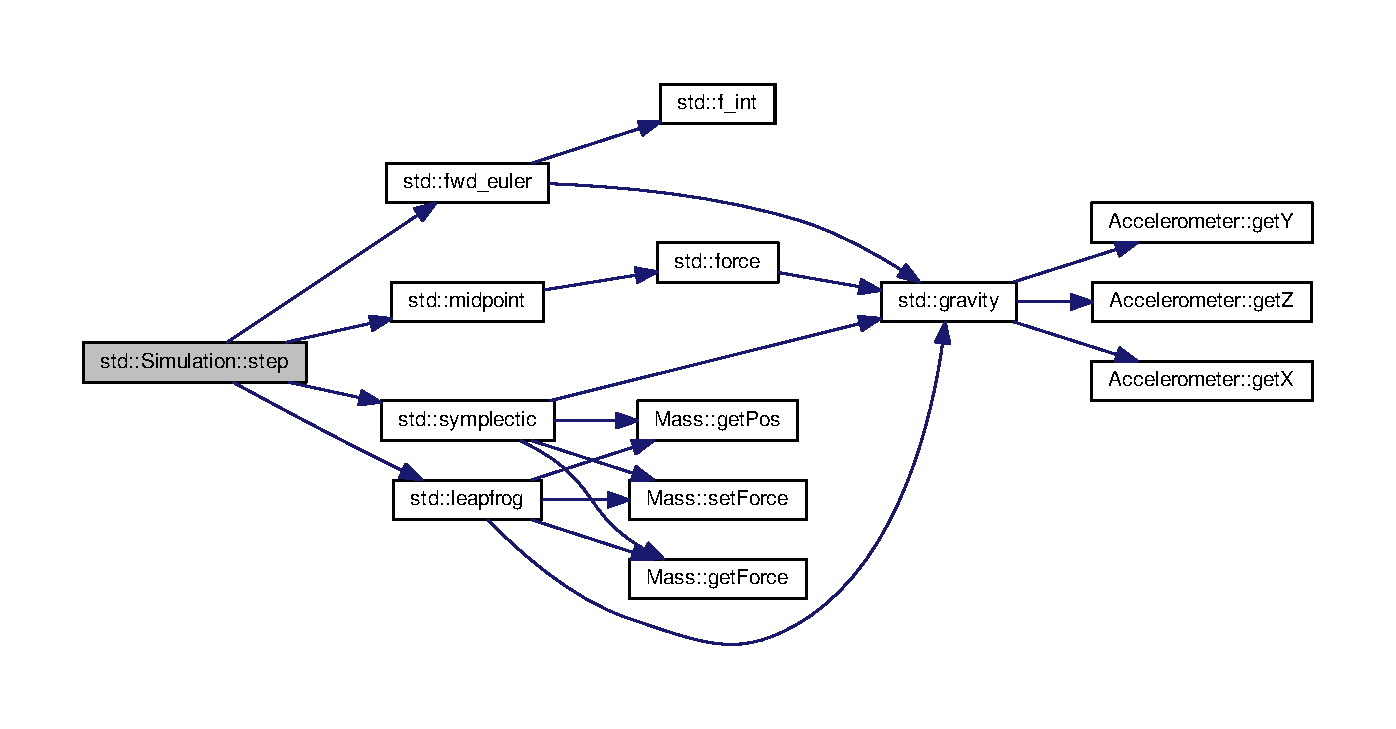
\includegraphics[width=350pt]{classstd_1_1Simulation_a0e50b0ce3a31b7ac77cf99b1aa7e3d62_cgraph}
\end{center}
\end{figure}




The documentation for this class was generated from the following files\+:\begin{DoxyCompactItemize}
\item 
src/\hyperlink{Simulation_8h}{Simulation.\+h}\item 
src/\hyperlink{Simulation_8cpp}{Simulation.\+cpp}\end{DoxyCompactItemize}

\hypertarget{classSpring}{}\section{Spring Class Reference}
\label{classSpring}\index{Spring@{Spring}}


{\ttfamily \#include $<$Spring.\+h$>$}



Collaboration diagram for Spring\+:\nopagebreak
\begin{figure}[H]
\begin{center}
\leavevmode
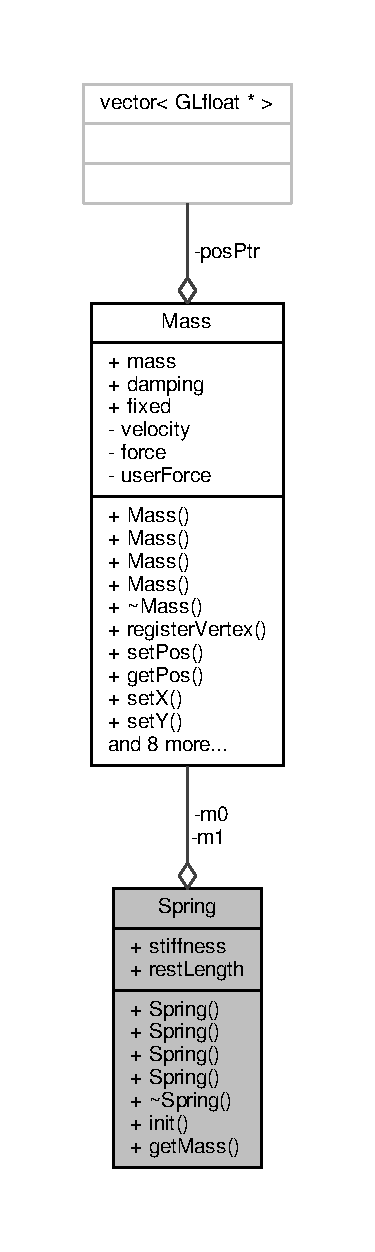
\includegraphics[height=550pt]{classSpring__coll__graph}
\end{center}
\end{figure}
\subsection*{Public Member Functions}
\begin{DoxyCompactItemize}
\item 
\hyperlink{classSpring_ae69e4d641c622ff4bc839583ba53bfdb}{Spring} (double stiff=0.\+0, double rest\+Len=0.\+0)
\item 
\hyperlink{classSpring_ac7d4d41e27e14f7cf5cd293cc38df645}{Spring} (\hyperlink{classMass}{Mass} $\ast$mass0, \hyperlink{classMass}{Mass} $\ast$mass1, double stiff=0.\+0, double rest\+Len=0.\+0)
\item 
\hyperlink{classSpring_a613221adae8bbcb7d64850e58d8646c6}{Spring} (\hyperlink{classSpring}{Spring} \&s)
\item 
\hyperlink{classSpring_aba1c60d6b08ffd72dc8560d657d8b703}{Spring} (\hyperlink{classSpring}{Spring} \&\&s)
\item 
virtual \hyperlink{classSpring_a8a9311f8a7cce2868498ad3da5d9c4b8}{$\sim$\+Spring} (void)
\item 
void \hyperlink{classSpring_a274a8d1cdb7de865bbf90ad6d95d789f}{init} (\hyperlink{classMass}{Mass} $\ast$mass0, \hyperlink{classMass}{Mass} $\ast$mass1)
\item 
\hyperlink{classMass}{Mass} $\ast$ \hyperlink{classSpring_a737bbcb5fe53e65b2afbb9c62dc3186f}{get\+Mass} (int i)
\end{DoxyCompactItemize}
\subsection*{Public Attributes}
\begin{DoxyCompactItemize}
\item 
double \hyperlink{classSpring_aed22a149191c40dcef27af3e029e60fd}{stiffness}
\item 
double \hyperlink{classSpring_ab2e2b4c400fcd277234b297f4f8cfd28}{rest\+Length}
\end{DoxyCompactItemize}
\subsection*{Private Attributes}
\begin{DoxyCompactItemize}
\item 
\hyperlink{classMass}{Mass} $\ast$ \hyperlink{classSpring_a59fda4f49a5645908643319198f4206f}{m0}
\item 
\hyperlink{classMass}{Mass} $\ast$ \hyperlink{classSpring_ac7909ea9cf093d7f267982a5ec3c51c6}{m1}
\end{DoxyCompactItemize}


\subsection{Detailed Description}
This class contains all properties of a spring which are necessary to run a physically based simulation of a mass-\/spring system. 

\subsection{Constructor \& Destructor Documentation}
\hypertarget{classSpring_ae69e4d641c622ff4bc839583ba53bfdb}{}\index{Spring@{Spring}!Spring@{Spring}}
\index{Spring@{Spring}!Spring@{Spring}}
\subsubsection[{Spring}]{\setlength{\rightskip}{0pt plus 5cm}Spring\+::\+Spring (
\begin{DoxyParamCaption}
\item[{double}]{stiff = {\ttfamily 0.0}, }
\item[{double}]{rest\+Len = {\ttfamily 0.0}}
\end{DoxyParamCaption}
)}\label{classSpring_ae69e4d641c622ff4bc839583ba53bfdb}
Default constructor.

The end-\/points are left uninitialized, so after calling this constructor a call to {\ttfamily \hyperlink{classSpring_a274a8d1cdb7de865bbf90ad6d95d789f}{init()}} is necessary. 
\begin{DoxyParams}{Parameters}
{\em stiff} & stiffness factor of the spring \\
\hline
{\em rest\+Len} & the rest length = length of the spring without any forces taking effect to it \\
\hline
\end{DoxyParams}
\hypertarget{classSpring_ac7d4d41e27e14f7cf5cd293cc38df645}{}\index{Spring@{Spring}!Spring@{Spring}}
\index{Spring@{Spring}!Spring@{Spring}}
\subsubsection[{Spring}]{\setlength{\rightskip}{0pt plus 5cm}Spring\+::\+Spring (
\begin{DoxyParamCaption}
\item[{{\bf Mass} $\ast$}]{mass0, }
\item[{{\bf Mass} $\ast$}]{mass1, }
\item[{double}]{stiff = {\ttfamily 0.0}, }
\item[{double}]{rest\+Len = {\ttfamily 0.0}}
\end{DoxyParamCaption}
)}\label{classSpring_ac7d4d41e27e14f7cf5cd293cc38df645}
Constructor which initializes the endpoints of the spring with two mass-\/points 
\begin{DoxyParams}{Parameters}
{\em mass0} & mass-\/point on the first end of the spring \\
\hline
{\em mass1} & mass-\/point on the second end \\
\hline
{\em stiff} & stiffness factor of the spring \\
\hline
{\em rest\+Len} & the rest length = length of the spring without any forces taking effect to it \\
\hline
\end{DoxyParams}
\hypertarget{classSpring_a613221adae8bbcb7d64850e58d8646c6}{}\index{Spring@{Spring}!Spring@{Spring}}
\index{Spring@{Spring}!Spring@{Spring}}
\subsubsection[{Spring}]{\setlength{\rightskip}{0pt plus 5cm}Spring\+::\+Spring (
\begin{DoxyParamCaption}
\item[{{\bf Spring} \&}]{s}
\end{DoxyParamCaption}
)}\label{classSpring_a613221adae8bbcb7d64850e58d8646c6}
Copy Constructor 
\begin{DoxyParams}{Parameters}
{\em s} & source spring \\
\hline
\end{DoxyParams}
\hypertarget{classSpring_aba1c60d6b08ffd72dc8560d657d8b703}{}\index{Spring@{Spring}!Spring@{Spring}}
\index{Spring@{Spring}!Spring@{Spring}}
\subsubsection[{Spring}]{\setlength{\rightskip}{0pt plus 5cm}Spring\+::\+Spring (
\begin{DoxyParamCaption}
\item[{{\bf Spring} \&\&}]{s}
\end{DoxyParamCaption}
)}\label{classSpring_aba1c60d6b08ffd72dc8560d657d8b703}
Move constructor 
\begin{DoxyParams}{Parameters}
{\em s} & source spring \\
\hline
\end{DoxyParams}
\hypertarget{classSpring_a8a9311f8a7cce2868498ad3da5d9c4b8}{}\index{Spring@{Spring}!````~Spring@{$\sim$\+Spring}}
\index{````~Spring@{$\sim$\+Spring}!Spring@{Spring}}
\subsubsection[{$\sim$\+Spring}]{\setlength{\rightskip}{0pt plus 5cm}Spring\+::$\sim$\+Spring (
\begin{DoxyParamCaption}
\item[{void}]{}
\end{DoxyParamCaption}
)\hspace{0.3cm}{\ttfamily [virtual]}}\label{classSpring_a8a9311f8a7cce2868498ad3da5d9c4b8}
Default destructor. 

\subsection{Member Function Documentation}
\hypertarget{classSpring_a737bbcb5fe53e65b2afbb9c62dc3186f}{}\index{Spring@{Spring}!get\+Mass@{get\+Mass}}
\index{get\+Mass@{get\+Mass}!Spring@{Spring}}
\subsubsection[{get\+Mass}]{\setlength{\rightskip}{0pt plus 5cm}{\bf Mass} $\ast$ Spring\+::get\+Mass (
\begin{DoxyParamCaption}
\item[{int}]{i}
\end{DoxyParamCaption}
)}\label{classSpring_a737bbcb5fe53e65b2afbb9c62dc3186f}
Get a mass. 
\begin{DoxyParams}{Parameters}
{\em i} & 0 or 1 to select the mass \\
\hline
\end{DoxyParams}
\begin{DoxyReturn}{Returns}
the selected mass 
\end{DoxyReturn}
\hypertarget{classSpring_a274a8d1cdb7de865bbf90ad6d95d789f}{}\index{Spring@{Spring}!init@{init}}
\index{init@{init}!Spring@{Spring}}
\subsubsection[{init}]{\setlength{\rightskip}{0pt plus 5cm}void Spring\+::init (
\begin{DoxyParamCaption}
\item[{{\bf Mass} $\ast$}]{mass0, }
\item[{{\bf Mass} $\ast$}]{mass1}
\end{DoxyParamCaption}
)}\label{classSpring_a274a8d1cdb7de865bbf90ad6d95d789f}
Initialize spring with two given masses and set the rest length to the distance of the two points. 
\begin{DoxyParams}{Parameters}
{\em mass0} & mass at end-\/point \\
\hline
{\em mass1} & mass at end-\/point \\
\hline
\end{DoxyParams}


Here is the call graph for this function\+:\nopagebreak
\begin{figure}[H]
\begin{center}
\leavevmode
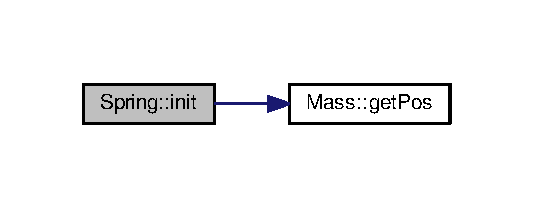
\includegraphics[width=256pt]{classSpring_a274a8d1cdb7de865bbf90ad6d95d789f_cgraph}
\end{center}
\end{figure}




\subsection{Member Data Documentation}
\hypertarget{classSpring_a59fda4f49a5645908643319198f4206f}{}\index{Spring@{Spring}!m0@{m0}}
\index{m0@{m0}!Spring@{Spring}}
\subsubsection[{m0}]{\setlength{\rightskip}{0pt plus 5cm}{\bf Mass}$\ast$ Spring\+::m0\hspace{0.3cm}{\ttfamily [private]}}\label{classSpring_a59fda4f49a5645908643319198f4206f}
\hypertarget{classSpring_ac7909ea9cf093d7f267982a5ec3c51c6}{}\index{Spring@{Spring}!m1@{m1}}
\index{m1@{m1}!Spring@{Spring}}
\subsubsection[{m1}]{\setlength{\rightskip}{0pt plus 5cm}{\bf Mass} $\ast$ Spring\+::m1\hspace{0.3cm}{\ttfamily [private]}}\label{classSpring_ac7909ea9cf093d7f267982a5ec3c51c6}
\hypertarget{classSpring_ab2e2b4c400fcd277234b297f4f8cfd28}{}\index{Spring@{Spring}!rest\+Length@{rest\+Length}}
\index{rest\+Length@{rest\+Length}!Spring@{Spring}}
\subsubsection[{rest\+Length}]{\setlength{\rightskip}{0pt plus 5cm}double Spring\+::rest\+Length}\label{classSpring_ab2e2b4c400fcd277234b297f4f8cfd28}
\hypertarget{classSpring_aed22a149191c40dcef27af3e029e60fd}{}\index{Spring@{Spring}!stiffness@{stiffness}}
\index{stiffness@{stiffness}!Spring@{Spring}}
\subsubsection[{stiffness}]{\setlength{\rightskip}{0pt plus 5cm}double Spring\+::stiffness}\label{classSpring_aed22a149191c40dcef27af3e029e60fd}


The documentation for this class was generated from the following files\+:\begin{DoxyCompactItemize}
\item 
src/\hyperlink{Spring_8h}{Spring.\+h}\item 
src/\hyperlink{Spring_8cpp}{Spring.\+cpp}\end{DoxyCompactItemize}

\chapter{File Documentation}
\hypertarget{Accelerometer_8cpp}{}\section{src/\+Accelerometer.cpp File Reference}
\label{Accelerometer_8cpp}\index{src/\+Accelerometer.\+cpp@{src/\+Accelerometer.\+cpp}}
{\ttfamily \#include $<$thread$>$}\\*
{\ttfamily \#include $<$mutex$>$}\\*
{\ttfamily \#include $<$iostream$>$}\\*
{\ttfamily \#include $<$fstream$>$}\\*
{\ttfamily \#include $<$cstring$>$}\\*
{\ttfamily \#include \char`\"{}Resource\+Path.\+h\char`\"{}}\\*
{\ttfamily \#include \char`\"{}Accelerometer.\+h\char`\"{}}\\*
Include dependency graph for Accelerometer.\+cpp\+:\nopagebreak
\begin{figure}[H]
\begin{center}
\leavevmode
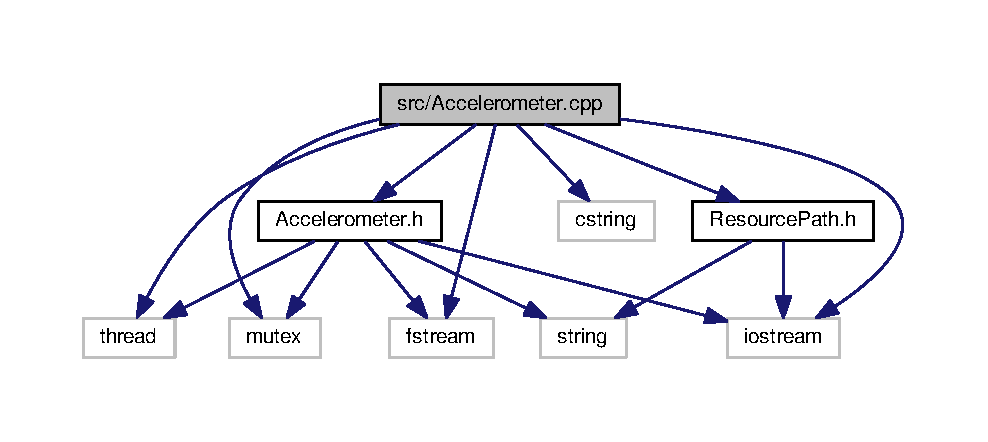
\includegraphics[width=350pt]{Accelerometer_8cpp__incl}
\end{center}
\end{figure}
\subsection*{Macros}
\begin{DoxyCompactItemize}
\item 
\#define \hyperlink{Accelerometer_8cpp_a06c158f5e120ed19ebbe820b9f274823}{\+\_\+\+P\+R\+I\+V\+\_\+\+L\+I\+N\+E\+\_\+\+L\+E\+N}~100
\end{DoxyCompactItemize}


\subsection{Macro Definition Documentation}
\hypertarget{Accelerometer_8cpp_a06c158f5e120ed19ebbe820b9f274823}{}\index{Accelerometer.\+cpp@{Accelerometer.\+cpp}!\+\_\+\+P\+R\+I\+V\+\_\+\+L\+I\+N\+E\+\_\+\+L\+E\+N@{\+\_\+\+P\+R\+I\+V\+\_\+\+L\+I\+N\+E\+\_\+\+L\+E\+N}}
\index{\+\_\+\+P\+R\+I\+V\+\_\+\+L\+I\+N\+E\+\_\+\+L\+E\+N@{\+\_\+\+P\+R\+I\+V\+\_\+\+L\+I\+N\+E\+\_\+\+L\+E\+N}!Accelerometer.\+cpp@{Accelerometer.\+cpp}}
\subsubsection[{\+\_\+\+P\+R\+I\+V\+\_\+\+L\+I\+N\+E\+\_\+\+L\+E\+N}]{\setlength{\rightskip}{0pt plus 5cm}\#define \+\_\+\+P\+R\+I\+V\+\_\+\+L\+I\+N\+E\+\_\+\+L\+E\+N~100}\label{Accelerometer_8cpp_a06c158f5e120ed19ebbe820b9f274823}

\hypertarget{Accelerometer_8h}{}\section{src/\+Accelerometer.h File Reference}
\label{Accelerometer_8h}\index{src/\+Accelerometer.\+h@{src/\+Accelerometer.\+h}}
{\ttfamily \#include $<$iostream$>$}\\*
{\ttfamily \#include $<$fstream$>$}\\*
{\ttfamily \#include $<$thread$>$}\\*
{\ttfamily \#include $<$mutex$>$}\\*
{\ttfamily \#include $<$string$>$}\\*
Include dependency graph for Accelerometer.\+h\+:\nopagebreak
\begin{figure}[H]
\begin{center}
\leavevmode
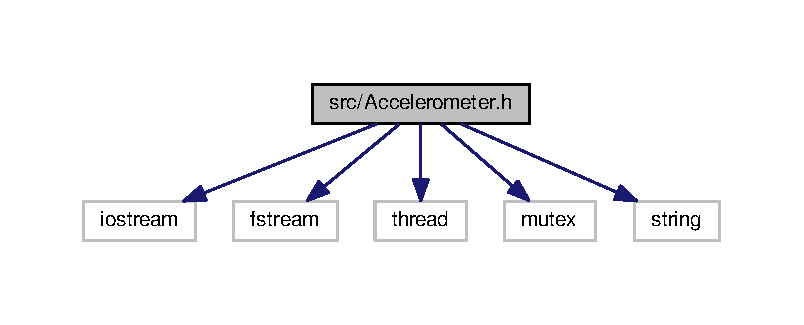
\includegraphics[width=350pt]{Accelerometer_8h__incl}
\end{center}
\end{figure}
This graph shows which files directly or indirectly include this file\+:\nopagebreak
\begin{figure}[H]
\begin{center}
\leavevmode
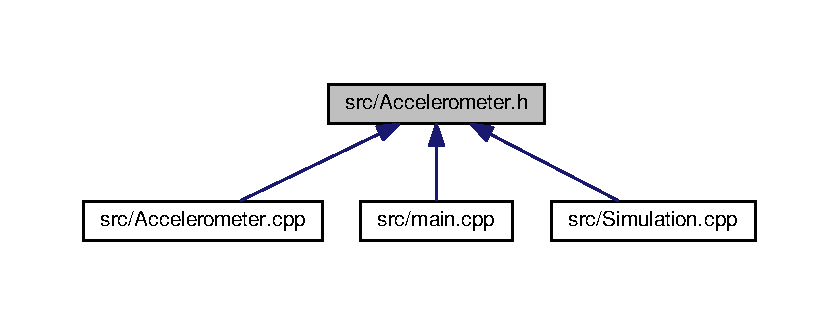
\includegraphics[width=350pt]{Accelerometer_8h__dep__incl}
\end{center}
\end{figure}
\subsection*{Classes}
\begin{DoxyCompactItemize}
\item 
class \hyperlink{classAccelerometer}{Accelerometer}
\end{DoxyCompactItemize}
\subsection*{Macros}
\begin{DoxyCompactItemize}
\item 
\#define \hyperlink{Accelerometer_8h_abcb20d5a1112ea44c7578c3b211462e3}{C\+F\+G\+\_\+\+F\+I\+L\+E\+N\+A\+M\+E}~\char`\"{}accelerometer.\+config\char`\"{}
\end{DoxyCompactItemize}


\subsection{Macro Definition Documentation}
\hypertarget{Accelerometer_8h_abcb20d5a1112ea44c7578c3b211462e3}{}\index{Accelerometer.\+h@{Accelerometer.\+h}!C\+F\+G\+\_\+\+F\+I\+L\+E\+N\+A\+M\+E@{C\+F\+G\+\_\+\+F\+I\+L\+E\+N\+A\+M\+E}}
\index{C\+F\+G\+\_\+\+F\+I\+L\+E\+N\+A\+M\+E@{C\+F\+G\+\_\+\+F\+I\+L\+E\+N\+A\+M\+E}!Accelerometer.\+h@{Accelerometer.\+h}}
\subsubsection[{C\+F\+G\+\_\+\+F\+I\+L\+E\+N\+A\+M\+E}]{\setlength{\rightskip}{0pt plus 5cm}\#define C\+F\+G\+\_\+\+F\+I\+L\+E\+N\+A\+M\+E~\char`\"{}accelerometer.\+config\char`\"{}}\label{Accelerometer_8h_abcb20d5a1112ea44c7578c3b211462e3}
This definition contains the hard-\/coded path to the device-\/config-\/file. T\+O\+D\+O. do it in a generic way -\/ some changes may be necessary to maintain multiple devices 
\hypertarget{Collision_8cpp}{}\section{src/\+Collision.cpp File Reference}
\label{Collision_8cpp}\index{src/\+Collision.\+cpp@{src/\+Collision.\+cpp}}
{\ttfamily \#include $<$iostream$>$}\\*
{\ttfamily \#include $<$vector$>$}\\*
{\ttfamily \#include $<$cmath$>$}\\*
{\ttfamily \#include $<$Eigen/\+Dense$>$}\\*
{\ttfamily \#include $<$G\+L/gl.\+h$>$}\\*
{\ttfamily \#include \char`\"{}Collision.\+h\char`\"{}}\\*
{\ttfamily \#include \char`\"{}Mass.\+h\char`\"{}}\\*
Include dependency graph for Collision.\+cpp\+:\nopagebreak
\begin{figure}[H]
\begin{center}
\leavevmode
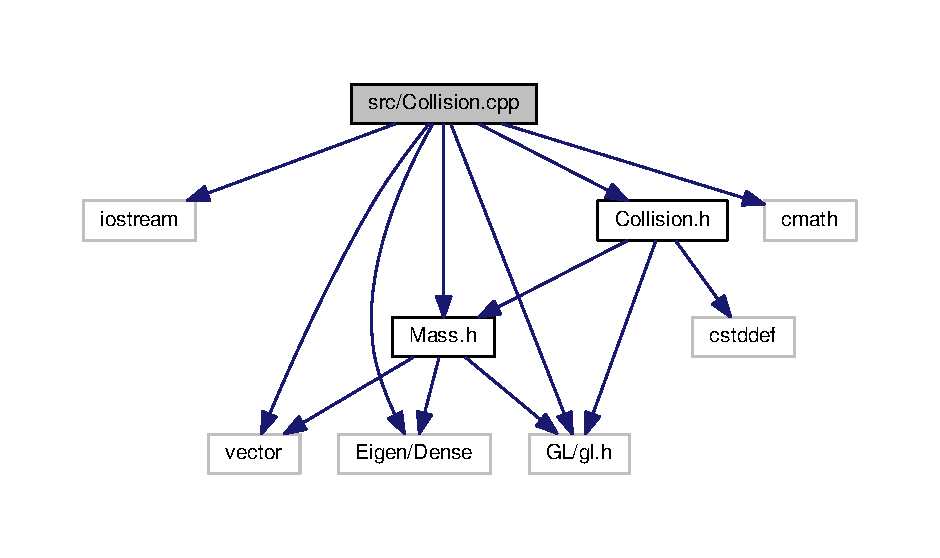
\includegraphics[width=350pt]{Collision_8cpp__incl}
\end{center}
\end{figure}
\subsection*{Namespaces}
\begin{DoxyCompactItemize}
\item 
 \hyperlink{namespacestd}{std}
\end{DoxyCompactItemize}
\subsection*{Functions}
\begin{DoxyCompactItemize}
\item 
bool \hyperlink{namespacestd_a8f17d2dea5f0758f77d130979a6ce6bf}{std\+::vertex\+In\+Triangle} (const Eigen\+::\+Vector3d \&P, const Eigen\+::\+Vector3d \&A, const Eigen\+::\+Vector3d \&B, const Eigen\+::\+Vector3d \&C, const float epsilon, float \&dist, Eigen\+::\+Vector3d \&N)
\item 
bool \hyperlink{namespacestd_a41fa9cfdd951bf0cc7f23973beaa7fdb}{std\+::bary\+Vertex\+In\+Triangle} (const Eigen\+::\+Vector3d \&P, const Eigen\+::\+Vector3d \&A, const Eigen\+::\+Vector3d \&B, const Eigen\+::\+Vector3d \&C)
\item 
void \hyperlink{namespacestd_a21cb14ca4c41a856be94b8fc9ff59c5a}{std\+::collision\+Detection\+And\+Response} (vector$<$ \hyperlink{classMass}{Mass} $>$ \&points, size\+\_\+t offs\+P, size\+\_\+t len\+P, G\+Lfloat object\+\_\+mesh\mbox{[}$\,$\mbox{]}, size\+\_\+t offs\+O, size\+\_\+t len\+O)
\end{DoxyCompactItemize}

\hypertarget{Collision_8h}{}\section{src/\+Collision.h File Reference}
\label{Collision_8h}\index{src/\+Collision.\+h@{src/\+Collision.\+h}}
{\ttfamily \#include $<$G\+L/gl.\+h$>$}\\*
{\ttfamily \#include $<$cstddef$>$}\\*
{\ttfamily \#include \char`\"{}Mass.\+h\char`\"{}}\\*
Include dependency graph for Collision.\+h\+:\nopagebreak
\begin{figure}[H]
\begin{center}
\leavevmode
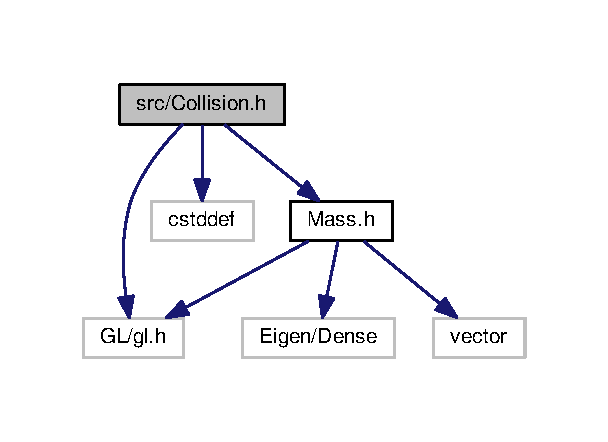
\includegraphics[width=292pt]{Collision_8h__incl}
\end{center}
\end{figure}
This graph shows which files directly or indirectly include this file\+:\nopagebreak
\begin{figure}[H]
\begin{center}
\leavevmode
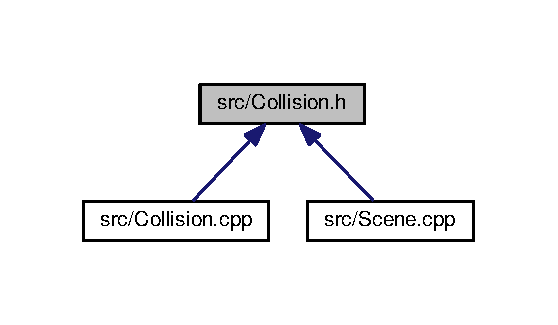
\includegraphics[width=268pt]{Collision_8h__dep__incl}
\end{center}
\end{figure}
\subsection*{Namespaces}
\begin{DoxyCompactItemize}
\item 
 \hyperlink{namespacestd}{std}
\end{DoxyCompactItemize}
\subsection*{Functions}
\begin{DoxyCompactItemize}
\item 
void \hyperlink{namespacestd_a21cb14ca4c41a856be94b8fc9ff59c5a}{std\+::collision\+Detection\+And\+Response} (vector$<$ \hyperlink{classMass}{Mass} $>$ \&points, size\+\_\+t offs\+P, size\+\_\+t len\+P, G\+Lfloat object\+\_\+mesh\mbox{[}$\,$\mbox{]}, size\+\_\+t offs\+O, size\+\_\+t len\+O)
\end{DoxyCompactItemize}


\subsection{Detailed Description}
This is a header file to include the functions needed for the collision detection algorithm. 
\hypertarget{dice_8c}{}\section{src/dice.c File Reference}
\label{dice_8c}\index{src/dice.\+c@{src/dice.\+c}}
{\ttfamily \#include $<$stddef.\+h$>$}\\*
{\ttfamily \#include $<$G\+L/gl.\+h$>$}\\*
{\ttfamily \#include \char`\"{}dice.\+h\char`\"{}}\\*
Include dependency graph for dice.\+c\+:\nopagebreak
\begin{figure}[H]
\begin{center}
\leavevmode
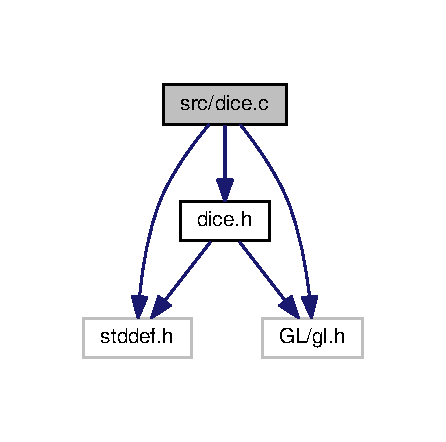
\includegraphics[width=214pt]{dice_8c__incl}
\end{center}
\end{figure}
\subsection*{Variables}
\begin{DoxyCompactItemize}
\item 
const size\+\_\+t \hyperlink{dice_8c_aadb2131969293f873d1ad5afc390f758}{dice\+Vertices} = 78
\item 
G\+Lfloat \hyperlink{dice_8c_ae0ea6da5fe2c1d7bccb52f18a41e9e5f}{dice\+Positions} \mbox{[}234\mbox{]}
\item 
G\+Lfloat \hyperlink{dice_8c_a57b46804d1b1e5cd7dcb056fedaf3d0d}{dice\+Texels} \mbox{[}156\mbox{]}
\item 
G\+Lfloat \hyperlink{dice_8c_a6a2708a2cb629b805ce3aeec64c252df}{dice\+Normals} \mbox{[}234\mbox{]}
\item 
const size\+\_\+t \hyperlink{dice_8c_a4d2afca4fccbc7967d7216539391e5ea}{dice\+Objects\+With\+Mass} = 2
\item 
const size\+\_\+t \hyperlink{dice_8c_af446084555dabc98d40fe6c825071792}{dice\+Masses} \mbox{[}2\mbox{]}
\item 
const size\+\_\+t \hyperlink{dice_8c_a2256021b0b6b805513f1107594c26fac}{dice\+Mass\+Fwd\+Offs} \mbox{[}2\mbox{]}
\item 
const size\+\_\+t \hyperlink{dice_8c_afc003c18ccbad7053176a220fb2ba3bf}{dice\+Mass\+Vertices} \mbox{[}2\mbox{]}
\item 
const size\+\_\+t \hyperlink{dice_8c_a2cc6d2cbe0fb31f9f17dea30abbfbfe3}{dice\+Mass\+Rev\+Offs} \mbox{[}2\mbox{]}
\item 
const size\+\_\+t \hyperlink{dice_8c_a0894ea6172a7fe5d0d4ced09bb7bbce0}{dice\+Mass\+Rev\+Offs\+Orig} \mbox{[}2\mbox{]}
\item 
const size\+\_\+t \hyperlink{dice_8c_aeacfb6aff4516202ff41ef3526f5ec17}{dice\+Fwd\+Index\+I} \mbox{[}72\mbox{]}
\item 
const size\+\_\+t $\ast$ \hyperlink{dice_8c_a008b85911456de4da8f11d0c8c361960}{dice\+Fwd\+Index} \mbox{[}16\mbox{]}
\item 
const size\+\_\+t \hyperlink{dice_8c_a0b5984db198523e421624a64a32d27a6}{dice\+Fwd\+Index\+Length} \mbox{[}16\mbox{]}
\item 
const size\+\_\+t \hyperlink{dice_8c_a151d4cc385afe602fe63029a3d2f8c72}{dice\+Rev\+Index} \mbox{[}72\mbox{]}
\item 
const size\+\_\+t \hyperlink{dice_8c_a95c05be2ec1d8199c405524c55576ae0}{dice\+Objects} = 3
\item 
const size\+\_\+t \hyperlink{dice_8c_adcd16a4c099cdc1cc4c75dd090d15ac0}{dice\+Object\+Offset} \mbox{[}3\mbox{]}
\item 
const size\+\_\+t \hyperlink{dice_8c_a665ab56567cdd39fca232f2a419e1596}{dice\+Object\+Length} \mbox{[}3\mbox{]}
\item 
const char \hyperlink{dice_8c_a01ece6ed8608732e272c5ac8221da2b7}{dice\+Object\+Names\+String} \mbox{[}36\mbox{]}
\item 
const char $\ast$ \hyperlink{dice_8c_aa7e6988a4ed1c68ec723a27a6bb8f139}{dice\+Object\+Names} \mbox{[}3\mbox{]}
\item 
const char \hyperlink{dice_8c_aa9a6cc0cda3677ec53bb02d138fbb54b}{dice\+Texture\+File\+Path} \mbox{[}34\mbox{]} = \char`\"{}/not\+\_\+implemented\+\_\+yet/edit/by.\+hand\char`\"{}
\end{DoxyCompactItemize}


\subsection{Detailed Description}
This is a C-\/source file (.c) for the models \char`\"{}dice\+\_\+\+Plane\char`\"{}, \char`\"{}dice\+\_\+\+Rolling\+Die\char`\"{}, \char`\"{}dice\+\_\+\+Die\char`\"{} Don\textquotesingle{}t edit! This is an auto-\/generated file by blender2o\+G\+L. Modifications are not permanent. 

\subsection{Variable Documentation}
\hypertarget{dice_8c_a008b85911456de4da8f11d0c8c361960}{}\index{dice.\+c@{dice.\+c}!dice\+Fwd\+Index@{dice\+Fwd\+Index}}
\index{dice\+Fwd\+Index@{dice\+Fwd\+Index}!dice.\+c@{dice.\+c}}
\subsubsection[{dice\+Fwd\+Index}]{\setlength{\rightskip}{0pt plus 5cm}const size\+\_\+t$\ast$ dice\+Fwd\+Index\mbox{[}16\mbox{]}}\label{dice_8c_a008b85911456de4da8f11d0c8c361960}
{\bfseries Initial value\+:}
\begin{DoxyCode}
= \{
    &\hyperlink{dice_8c_aeacfb6aff4516202ff41ef3526f5ec17}{diceFwdIndexI}[0],
    &\hyperlink{dice_8c_aeacfb6aff4516202ff41ef3526f5ec17}{diceFwdIndexI}[5],
    &diceFwdIndexI[9],
    &diceFwdIndexI[14],
    &diceFwdIndexI[18],
    &diceFwdIndexI[23],
    &diceFwdIndexI[27],
    &diceFwdIndexI[32],
    &diceFwdIndexI[36],
    &diceFwdIndexI[41],
    &diceFwdIndexI[45],
    &diceFwdIndexI[50],
    &diceFwdIndexI[54],
    &diceFwdIndexI[59],
    &diceFwdIndexI[63],
    &diceFwdIndexI[68],
\}
\end{DoxyCode}
\hypertarget{dice_8c_aeacfb6aff4516202ff41ef3526f5ec17}{}\index{dice.\+c@{dice.\+c}!dice\+Fwd\+Index\+I@{dice\+Fwd\+Index\+I}}
\index{dice\+Fwd\+Index\+I@{dice\+Fwd\+Index\+I}!dice.\+c@{dice.\+c}}
\subsubsection[{dice\+Fwd\+Index\+I}]{\setlength{\rightskip}{0pt plus 5cm}const size\+\_\+t dice\+Fwd\+Index\+I\mbox{[}72\mbox{]}}\label{dice_8c_aeacfb6aff4516202ff41ef3526f5ec17}
{\bfseries Initial value\+:}
\begin{DoxyCode}
= \{
    6, 9, 18, 21, 37,
    7, 23, 24, 27,
    8, 10, 29, 30, 33,
    11, 35, 38, 40,
    12, 15, 19, 36, 39,
    17, 20, 22, 25,
    14, 16, 26, 28, 31,
    13, 32, 34, 41,
    42, 45, 54, 57, 73,
    43, 59, 60, 63,
    44, 46, 65, 66, 69,
    47, 71, 74, 76,
    48, 51, 55, 72, 75,
    53, 56, 58, 61,
    50, 52, 62, 64, 67,
    49, 68, 70, 77,
\}
\end{DoxyCode}
\hypertarget{dice_8c_a0b5984db198523e421624a64a32d27a6}{}\index{dice.\+c@{dice.\+c}!dice\+Fwd\+Index\+Length@{dice\+Fwd\+Index\+Length}}
\index{dice\+Fwd\+Index\+Length@{dice\+Fwd\+Index\+Length}!dice.\+c@{dice.\+c}}
\subsubsection[{dice\+Fwd\+Index\+Length}]{\setlength{\rightskip}{0pt plus 5cm}const size\+\_\+t dice\+Fwd\+Index\+Length\mbox{[}16\mbox{]}}\label{dice_8c_a0b5984db198523e421624a64a32d27a6}
{\bfseries Initial value\+:}
\begin{DoxyCode}
= \{
    5,
    4,
    5,
    4,
    5,
    4,
    5,
    4,
    5,
    4,
    5,
    4,
    5,
    4,
    5,
    4,
\}
\end{DoxyCode}
\hypertarget{dice_8c_af446084555dabc98d40fe6c825071792}{}\index{dice.\+c@{dice.\+c}!dice\+Masses@{dice\+Masses}}
\index{dice\+Masses@{dice\+Masses}!dice.\+c@{dice.\+c}}
\subsubsection[{dice\+Masses}]{\setlength{\rightskip}{0pt plus 5cm}const size\+\_\+t dice\+Masses\mbox{[}2\mbox{]}}\label{dice_8c_af446084555dabc98d40fe6c825071792}
{\bfseries Initial value\+:}
\begin{DoxyCode}
= \{
    8,
    8,
\}
\end{DoxyCode}
\hypertarget{dice_8c_a2256021b0b6b805513f1107594c26fac}{}\index{dice.\+c@{dice.\+c}!dice\+Mass\+Fwd\+Offs@{dice\+Mass\+Fwd\+Offs}}
\index{dice\+Mass\+Fwd\+Offs@{dice\+Mass\+Fwd\+Offs}!dice.\+c@{dice.\+c}}
\subsubsection[{dice\+Mass\+Fwd\+Offs}]{\setlength{\rightskip}{0pt plus 5cm}const size\+\_\+t dice\+Mass\+Fwd\+Offs\mbox{[}2\mbox{]}}\label{dice_8c_a2256021b0b6b805513f1107594c26fac}
{\bfseries Initial value\+:}
\begin{DoxyCode}
= \{
    0,
    8,
\}
\end{DoxyCode}
\hypertarget{dice_8c_a2cc6d2cbe0fb31f9f17dea30abbfbfe3}{}\index{dice.\+c@{dice.\+c}!dice\+Mass\+Rev\+Offs@{dice\+Mass\+Rev\+Offs}}
\index{dice\+Mass\+Rev\+Offs@{dice\+Mass\+Rev\+Offs}!dice.\+c@{dice.\+c}}
\subsubsection[{dice\+Mass\+Rev\+Offs}]{\setlength{\rightskip}{0pt plus 5cm}const size\+\_\+t dice\+Mass\+Rev\+Offs\mbox{[}2\mbox{]}}\label{dice_8c_a2cc6d2cbe0fb31f9f17dea30abbfbfe3}
{\bfseries Initial value\+:}
\begin{DoxyCode}
= \{
    0,
    36,
\}
\end{DoxyCode}
\hypertarget{dice_8c_a0894ea6172a7fe5d0d4ced09bb7bbce0}{}\index{dice.\+c@{dice.\+c}!dice\+Mass\+Rev\+Offs\+Orig@{dice\+Mass\+Rev\+Offs\+Orig}}
\index{dice\+Mass\+Rev\+Offs\+Orig@{dice\+Mass\+Rev\+Offs\+Orig}!dice.\+c@{dice.\+c}}
\subsubsection[{dice\+Mass\+Rev\+Offs\+Orig}]{\setlength{\rightskip}{0pt plus 5cm}const size\+\_\+t dice\+Mass\+Rev\+Offs\+Orig\mbox{[}2\mbox{]}}\label{dice_8c_a0894ea6172a7fe5d0d4ced09bb7bbce0}
{\bfseries Initial value\+:}
\begin{DoxyCode}
= \{
    6,
    42,
\}
\end{DoxyCode}
\hypertarget{dice_8c_afc003c18ccbad7053176a220fb2ba3bf}{}\index{dice.\+c@{dice.\+c}!dice\+Mass\+Vertices@{dice\+Mass\+Vertices}}
\index{dice\+Mass\+Vertices@{dice\+Mass\+Vertices}!dice.\+c@{dice.\+c}}
\subsubsection[{dice\+Mass\+Vertices}]{\setlength{\rightskip}{0pt plus 5cm}const size\+\_\+t dice\+Mass\+Vertices\mbox{[}2\mbox{]}}\label{dice_8c_afc003c18ccbad7053176a220fb2ba3bf}
{\bfseries Initial value\+:}
\begin{DoxyCode}
= \{
    36,
    36,
\}
\end{DoxyCode}
\hypertarget{dice_8c_a6a2708a2cb629b805ce3aeec64c252df}{}\index{dice.\+c@{dice.\+c}!dice\+Normals@{dice\+Normals}}
\index{dice\+Normals@{dice\+Normals}!dice.\+c@{dice.\+c}}
\subsubsection[{dice\+Normals}]{\setlength{\rightskip}{0pt plus 5cm}G\+Lfloat dice\+Normals\mbox{[}234\mbox{]}}\label{dice_8c_a6a2708a2cb629b805ce3aeec64c252df}
\hypertarget{dice_8c_a665ab56567cdd39fca232f2a419e1596}{}\index{dice.\+c@{dice.\+c}!dice\+Object\+Length@{dice\+Object\+Length}}
\index{dice\+Object\+Length@{dice\+Object\+Length}!dice.\+c@{dice.\+c}}
\subsubsection[{dice\+Object\+Length}]{\setlength{\rightskip}{0pt plus 5cm}const size\+\_\+t dice\+Object\+Length\mbox{[}3\mbox{]}}\label{dice_8c_a665ab56567cdd39fca232f2a419e1596}
{\bfseries Initial value\+:}
\begin{DoxyCode}
= \{
    6,
    36,
    36,
\}
\end{DoxyCode}
\hypertarget{dice_8c_aa7e6988a4ed1c68ec723a27a6bb8f139}{}\index{dice.\+c@{dice.\+c}!dice\+Object\+Names@{dice\+Object\+Names}}
\index{dice\+Object\+Names@{dice\+Object\+Names}!dice.\+c@{dice.\+c}}
\subsubsection[{dice\+Object\+Names}]{\setlength{\rightskip}{0pt plus 5cm}const char$\ast$ dice\+Object\+Names\mbox{[}3\mbox{]}}\label{dice_8c_aa7e6988a4ed1c68ec723a27a6bb8f139}
{\bfseries Initial value\+:}
\begin{DoxyCode}
= \{
    &\hyperlink{dice_8c_a01ece6ed8608732e272c5ac8221da2b7}{diceObjectNamesString}[0],
    &\hyperlink{dice_8c_a01ece6ed8608732e272c5ac8221da2b7}{diceObjectNamesString}[11],
    &diceObjectNamesString[27],
\}
\end{DoxyCode}
\hypertarget{dice_8c_a01ece6ed8608732e272c5ac8221da2b7}{}\index{dice.\+c@{dice.\+c}!dice\+Object\+Names\+String@{dice\+Object\+Names\+String}}
\index{dice\+Object\+Names\+String@{dice\+Object\+Names\+String}!dice.\+c@{dice.\+c}}
\subsubsection[{dice\+Object\+Names\+String}]{\setlength{\rightskip}{0pt plus 5cm}const char dice\+Object\+Names\+String\mbox{[}36\mbox{]}}\label{dice_8c_a01ece6ed8608732e272c5ac8221da2b7}
{\bfseries Initial value\+:}
\begin{DoxyCode}
= \{
    \textcolor{stringliteral}{"dice\_Plane\(\backslash\)0"}
    \textcolor{stringliteral}{"dice\_RollingDie\(\backslash\)0"}
    \textcolor{stringliteral}{"dice\_Die\(\backslash\)0"}
\}
\end{DoxyCode}
\hypertarget{dice_8c_adcd16a4c099cdc1cc4c75dd090d15ac0}{}\index{dice.\+c@{dice.\+c}!dice\+Object\+Offset@{dice\+Object\+Offset}}
\index{dice\+Object\+Offset@{dice\+Object\+Offset}!dice.\+c@{dice.\+c}}
\subsubsection[{dice\+Object\+Offset}]{\setlength{\rightskip}{0pt plus 5cm}const size\+\_\+t dice\+Object\+Offset\mbox{[}3\mbox{]}}\label{dice_8c_adcd16a4c099cdc1cc4c75dd090d15ac0}
{\bfseries Initial value\+:}
\begin{DoxyCode}
= \{
    0,
    6,
    42,
\}
\end{DoxyCode}
\hypertarget{dice_8c_a95c05be2ec1d8199c405524c55576ae0}{}\index{dice.\+c@{dice.\+c}!dice\+Objects@{dice\+Objects}}
\index{dice\+Objects@{dice\+Objects}!dice.\+c@{dice.\+c}}
\subsubsection[{dice\+Objects}]{\setlength{\rightskip}{0pt plus 5cm}const size\+\_\+t dice\+Objects = 3}\label{dice_8c_a95c05be2ec1d8199c405524c55576ae0}
\hypertarget{dice_8c_a4d2afca4fccbc7967d7216539391e5ea}{}\index{dice.\+c@{dice.\+c}!dice\+Objects\+With\+Mass@{dice\+Objects\+With\+Mass}}
\index{dice\+Objects\+With\+Mass@{dice\+Objects\+With\+Mass}!dice.\+c@{dice.\+c}}
\subsubsection[{dice\+Objects\+With\+Mass}]{\setlength{\rightskip}{0pt plus 5cm}const size\+\_\+t dice\+Objects\+With\+Mass = 2}\label{dice_8c_a4d2afca4fccbc7967d7216539391e5ea}
\hypertarget{dice_8c_ae0ea6da5fe2c1d7bccb52f18a41e9e5f}{}\index{dice.\+c@{dice.\+c}!dice\+Positions@{dice\+Positions}}
\index{dice\+Positions@{dice\+Positions}!dice.\+c@{dice.\+c}}
\subsubsection[{dice\+Positions}]{\setlength{\rightskip}{0pt plus 5cm}G\+Lfloat dice\+Positions\mbox{[}234\mbox{]}}\label{dice_8c_ae0ea6da5fe2c1d7bccb52f18a41e9e5f}
\hypertarget{dice_8c_a151d4cc385afe602fe63029a3d2f8c72}{}\index{dice.\+c@{dice.\+c}!dice\+Rev\+Index@{dice\+Rev\+Index}}
\index{dice\+Rev\+Index@{dice\+Rev\+Index}!dice.\+c@{dice.\+c}}
\subsubsection[{dice\+Rev\+Index}]{\setlength{\rightskip}{0pt plus 5cm}const size\+\_\+t dice\+Rev\+Index\mbox{[}72\mbox{]}}\label{dice_8c_a151d4cc385afe602fe63029a3d2f8c72}
{\bfseries Initial value\+:}
\begin{DoxyCode}
= \{
    0, 1, 2,
    0, 2, 3,
    4, 7, 6,
    4, 6, 5,
    0, 4, 5,
    0, 5, 1,
    1, 5, 6,
    1, 6, 2,
    2, 6, 7,
    2, 7, 3,
    4, 0, 3,
    4, 3, 7,
    8, 9, 10,
    8, 10, 11,
    12, 15, 14,
    12, 14, 13,
    8, 12, 13,
    8, 13, 9,
    9, 13, 14,
    9, 14, 10,
    10, 14, 15,
    10, 15, 11,
    12, 8, 11,
    12, 11, 15,
\}
\end{DoxyCode}
\hypertarget{dice_8c_a57b46804d1b1e5cd7dcb056fedaf3d0d}{}\index{dice.\+c@{dice.\+c}!dice\+Texels@{dice\+Texels}}
\index{dice\+Texels@{dice\+Texels}!dice.\+c@{dice.\+c}}
\subsubsection[{dice\+Texels}]{\setlength{\rightskip}{0pt plus 5cm}G\+Lfloat dice\+Texels\mbox{[}156\mbox{]}}\label{dice_8c_a57b46804d1b1e5cd7dcb056fedaf3d0d}
\hypertarget{dice_8c_aa9a6cc0cda3677ec53bb02d138fbb54b}{}\index{dice.\+c@{dice.\+c}!dice\+Texture\+File\+Path@{dice\+Texture\+File\+Path}}
\index{dice\+Texture\+File\+Path@{dice\+Texture\+File\+Path}!dice.\+c@{dice.\+c}}
\subsubsection[{dice\+Texture\+File\+Path}]{\setlength{\rightskip}{0pt plus 5cm}const char dice\+Texture\+File\+Path\mbox{[}34\mbox{]} = \char`\"{}/not\+\_\+implemented\+\_\+yet/edit/by.\+hand\char`\"{}}\label{dice_8c_aa9a6cc0cda3677ec53bb02d138fbb54b}
\hypertarget{dice_8c_aadb2131969293f873d1ad5afc390f758}{}\index{dice.\+c@{dice.\+c}!dice\+Vertices@{dice\+Vertices}}
\index{dice\+Vertices@{dice\+Vertices}!dice.\+c@{dice.\+c}}
\subsubsection[{dice\+Vertices}]{\setlength{\rightskip}{0pt plus 5cm}const size\+\_\+t dice\+Vertices = 78}\label{dice_8c_aadb2131969293f873d1ad5afc390f758}

\hypertarget{dice_8h}{}\section{src/dice.h File Reference}
\label{dice_8h}\index{src/dice.\+h@{src/dice.\+h}}
{\ttfamily \#include $<$G\+L/gl.\+h$>$}\\*
{\ttfamily \#include $<$stddef.\+h$>$}\\*
Include dependency graph for dice.\+h\+:\nopagebreak
\begin{figure}[H]
\begin{center}
\leavevmode
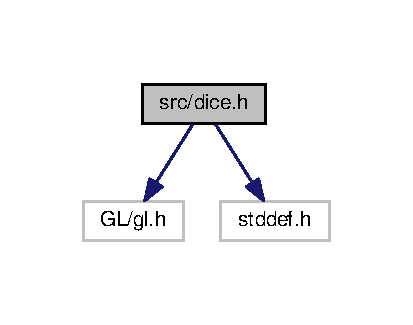
\includegraphics[width=198pt]{dice_8h__incl}
\end{center}
\end{figure}
This graph shows which files directly or indirectly include this file\+:\nopagebreak
\begin{figure}[H]
\begin{center}
\leavevmode
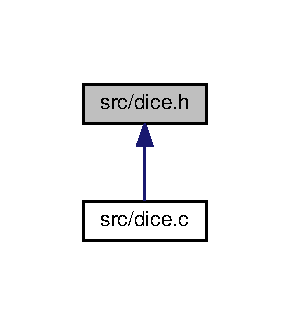
\includegraphics[width=139pt]{dice_8h__dep__incl}
\end{center}
\end{figure}
\subsection*{Variables}
\begin{DoxyCompactItemize}
\item 
const size\+\_\+t \hyperlink{dice_8h_aadb2131969293f873d1ad5afc390f758}{dice\+Vertices}
\item 
G\+Lfloat \hyperlink{dice_8h_ae0ea6da5fe2c1d7bccb52f18a41e9e5f}{dice\+Positions} \mbox{[}234\mbox{]}
\item 
G\+Lfloat \hyperlink{dice_8h_a57b46804d1b1e5cd7dcb056fedaf3d0d}{dice\+Texels} \mbox{[}156\mbox{]}
\item 
G\+Lfloat \hyperlink{dice_8h_a6a2708a2cb629b805ce3aeec64c252df}{dice\+Normals} \mbox{[}234\mbox{]}
\item 
const size\+\_\+t \hyperlink{dice_8h_a4d2afca4fccbc7967d7216539391e5ea}{dice\+Objects\+With\+Mass}
\item 
const size\+\_\+t \hyperlink{dice_8h_af446084555dabc98d40fe6c825071792}{dice\+Masses} \mbox{[}2\mbox{]}
\item 
const size\+\_\+t \hyperlink{dice_8h_a2256021b0b6b805513f1107594c26fac}{dice\+Mass\+Fwd\+Offs} \mbox{[}2\mbox{]}
\item 
const size\+\_\+t \hyperlink{dice_8h_afc003c18ccbad7053176a220fb2ba3bf}{dice\+Mass\+Vertices} \mbox{[}2\mbox{]}
\item 
const size\+\_\+t \hyperlink{dice_8h_a2cc6d2cbe0fb31f9f17dea30abbfbfe3}{dice\+Mass\+Rev\+Offs} \mbox{[}2\mbox{]}
\item 
const size\+\_\+t \hyperlink{dice_8h_a0894ea6172a7fe5d0d4ced09bb7bbce0}{dice\+Mass\+Rev\+Offs\+Orig} \mbox{[}2\mbox{]}
\item 
const size\+\_\+t \hyperlink{dice_8h_aeacfb6aff4516202ff41ef3526f5ec17}{dice\+Fwd\+Index\+I} \mbox{[}72\mbox{]}
\item 
const size\+\_\+t $\ast$ \hyperlink{dice_8h_a008b85911456de4da8f11d0c8c361960}{dice\+Fwd\+Index} \mbox{[}16\mbox{]}
\item 
const size\+\_\+t \hyperlink{dice_8h_a0b5984db198523e421624a64a32d27a6}{dice\+Fwd\+Index\+Length} \mbox{[}16\mbox{]}
\item 
const size\+\_\+t \hyperlink{dice_8h_a151d4cc385afe602fe63029a3d2f8c72}{dice\+Rev\+Index} \mbox{[}72\mbox{]}
\item 
const size\+\_\+t \hyperlink{dice_8h_a95c05be2ec1d8199c405524c55576ae0}{dice\+Objects}
\item 
const size\+\_\+t \hyperlink{dice_8h_adcd16a4c099cdc1cc4c75dd090d15ac0}{dice\+Object\+Offset} \mbox{[}3\mbox{]}
\item 
const size\+\_\+t \hyperlink{dice_8h_a665ab56567cdd39fca232f2a419e1596}{dice\+Object\+Length} \mbox{[}3\mbox{]}
\item 
const char \hyperlink{dice_8h_a01ece6ed8608732e272c5ac8221da2b7}{dice\+Object\+Names\+String} \mbox{[}36\mbox{]}
\item 
const char $\ast$ \hyperlink{dice_8h_aa7e6988a4ed1c68ec723a27a6bb8f139}{dice\+Object\+Names} \mbox{[}3\mbox{]}
\item 
const char \hyperlink{dice_8h_aa9a6cc0cda3677ec53bb02d138fbb54b}{dice\+Texture\+File\+Path} \mbox{[}34\mbox{]}
\end{DoxyCompactItemize}


\subsection{Detailed Description}
This is a C-\/header file (.h) for the models \char`\"{}dice\+\_\+\+Plane\char`\"{}, \char`\"{}dice\+\_\+\+Rolling\+Die\char`\"{}, \char`\"{}dice\+\_\+\+Die\char`\"{} Don\textquotesingle{}t edit! This is an auto-\/generated file by blender2o\+G\+L. Modifications are not permanent. 

\subsection{Variable Documentation}
\hypertarget{dice_8h_a008b85911456de4da8f11d0c8c361960}{}\index{dice.\+h@{dice.\+h}!dice\+Fwd\+Index@{dice\+Fwd\+Index}}
\index{dice\+Fwd\+Index@{dice\+Fwd\+Index}!dice.\+h@{dice.\+h}}
\subsubsection[{dice\+Fwd\+Index}]{\setlength{\rightskip}{0pt plus 5cm}const size\+\_\+t$\ast$ dice\+Fwd\+Index\mbox{[}16\mbox{]}}\label{dice_8h_a008b85911456de4da8f11d0c8c361960}
\hypertarget{dice_8h_aeacfb6aff4516202ff41ef3526f5ec17}{}\index{dice.\+h@{dice.\+h}!dice\+Fwd\+Index\+I@{dice\+Fwd\+Index\+I}}
\index{dice\+Fwd\+Index\+I@{dice\+Fwd\+Index\+I}!dice.\+h@{dice.\+h}}
\subsubsection[{dice\+Fwd\+Index\+I}]{\setlength{\rightskip}{0pt plus 5cm}const size\+\_\+t dice\+Fwd\+Index\+I\mbox{[}72\mbox{]}}\label{dice_8h_aeacfb6aff4516202ff41ef3526f5ec17}
\hypertarget{dice_8h_a0b5984db198523e421624a64a32d27a6}{}\index{dice.\+h@{dice.\+h}!dice\+Fwd\+Index\+Length@{dice\+Fwd\+Index\+Length}}
\index{dice\+Fwd\+Index\+Length@{dice\+Fwd\+Index\+Length}!dice.\+h@{dice.\+h}}
\subsubsection[{dice\+Fwd\+Index\+Length}]{\setlength{\rightskip}{0pt plus 5cm}const size\+\_\+t dice\+Fwd\+Index\+Length\mbox{[}16\mbox{]}}\label{dice_8h_a0b5984db198523e421624a64a32d27a6}
\hypertarget{dice_8h_af446084555dabc98d40fe6c825071792}{}\index{dice.\+h@{dice.\+h}!dice\+Masses@{dice\+Masses}}
\index{dice\+Masses@{dice\+Masses}!dice.\+h@{dice.\+h}}
\subsubsection[{dice\+Masses}]{\setlength{\rightskip}{0pt plus 5cm}const size\+\_\+t dice\+Masses\mbox{[}2\mbox{]}}\label{dice_8h_af446084555dabc98d40fe6c825071792}
\hypertarget{dice_8h_a2256021b0b6b805513f1107594c26fac}{}\index{dice.\+h@{dice.\+h}!dice\+Mass\+Fwd\+Offs@{dice\+Mass\+Fwd\+Offs}}
\index{dice\+Mass\+Fwd\+Offs@{dice\+Mass\+Fwd\+Offs}!dice.\+h@{dice.\+h}}
\subsubsection[{dice\+Mass\+Fwd\+Offs}]{\setlength{\rightskip}{0pt plus 5cm}const size\+\_\+t dice\+Mass\+Fwd\+Offs\mbox{[}2\mbox{]}}\label{dice_8h_a2256021b0b6b805513f1107594c26fac}
\hypertarget{dice_8h_a2cc6d2cbe0fb31f9f17dea30abbfbfe3}{}\index{dice.\+h@{dice.\+h}!dice\+Mass\+Rev\+Offs@{dice\+Mass\+Rev\+Offs}}
\index{dice\+Mass\+Rev\+Offs@{dice\+Mass\+Rev\+Offs}!dice.\+h@{dice.\+h}}
\subsubsection[{dice\+Mass\+Rev\+Offs}]{\setlength{\rightskip}{0pt plus 5cm}const size\+\_\+t dice\+Mass\+Rev\+Offs\mbox{[}2\mbox{]}}\label{dice_8h_a2cc6d2cbe0fb31f9f17dea30abbfbfe3}
\hypertarget{dice_8h_a0894ea6172a7fe5d0d4ced09bb7bbce0}{}\index{dice.\+h@{dice.\+h}!dice\+Mass\+Rev\+Offs\+Orig@{dice\+Mass\+Rev\+Offs\+Orig}}
\index{dice\+Mass\+Rev\+Offs\+Orig@{dice\+Mass\+Rev\+Offs\+Orig}!dice.\+h@{dice.\+h}}
\subsubsection[{dice\+Mass\+Rev\+Offs\+Orig}]{\setlength{\rightskip}{0pt plus 5cm}const size\+\_\+t dice\+Mass\+Rev\+Offs\+Orig\mbox{[}2\mbox{]}}\label{dice_8h_a0894ea6172a7fe5d0d4ced09bb7bbce0}
\hypertarget{dice_8h_afc003c18ccbad7053176a220fb2ba3bf}{}\index{dice.\+h@{dice.\+h}!dice\+Mass\+Vertices@{dice\+Mass\+Vertices}}
\index{dice\+Mass\+Vertices@{dice\+Mass\+Vertices}!dice.\+h@{dice.\+h}}
\subsubsection[{dice\+Mass\+Vertices}]{\setlength{\rightskip}{0pt plus 5cm}const size\+\_\+t dice\+Mass\+Vertices\mbox{[}2\mbox{]}}\label{dice_8h_afc003c18ccbad7053176a220fb2ba3bf}
\hypertarget{dice_8h_a6a2708a2cb629b805ce3aeec64c252df}{}\index{dice.\+h@{dice.\+h}!dice\+Normals@{dice\+Normals}}
\index{dice\+Normals@{dice\+Normals}!dice.\+h@{dice.\+h}}
\subsubsection[{dice\+Normals}]{\setlength{\rightskip}{0pt plus 5cm}G\+Lfloat dice\+Normals\mbox{[}234\mbox{]}}\label{dice_8h_a6a2708a2cb629b805ce3aeec64c252df}
\hypertarget{dice_8h_a665ab56567cdd39fca232f2a419e1596}{}\index{dice.\+h@{dice.\+h}!dice\+Object\+Length@{dice\+Object\+Length}}
\index{dice\+Object\+Length@{dice\+Object\+Length}!dice.\+h@{dice.\+h}}
\subsubsection[{dice\+Object\+Length}]{\setlength{\rightskip}{0pt plus 5cm}const size\+\_\+t dice\+Object\+Length\mbox{[}3\mbox{]}}\label{dice_8h_a665ab56567cdd39fca232f2a419e1596}
\hypertarget{dice_8h_aa7e6988a4ed1c68ec723a27a6bb8f139}{}\index{dice.\+h@{dice.\+h}!dice\+Object\+Names@{dice\+Object\+Names}}
\index{dice\+Object\+Names@{dice\+Object\+Names}!dice.\+h@{dice.\+h}}
\subsubsection[{dice\+Object\+Names}]{\setlength{\rightskip}{0pt plus 5cm}const char$\ast$ dice\+Object\+Names\mbox{[}3\mbox{]}}\label{dice_8h_aa7e6988a4ed1c68ec723a27a6bb8f139}
\hypertarget{dice_8h_a01ece6ed8608732e272c5ac8221da2b7}{}\index{dice.\+h@{dice.\+h}!dice\+Object\+Names\+String@{dice\+Object\+Names\+String}}
\index{dice\+Object\+Names\+String@{dice\+Object\+Names\+String}!dice.\+h@{dice.\+h}}
\subsubsection[{dice\+Object\+Names\+String}]{\setlength{\rightskip}{0pt plus 5cm}const char dice\+Object\+Names\+String\mbox{[}36\mbox{]}}\label{dice_8h_a01ece6ed8608732e272c5ac8221da2b7}
\hypertarget{dice_8h_adcd16a4c099cdc1cc4c75dd090d15ac0}{}\index{dice.\+h@{dice.\+h}!dice\+Object\+Offset@{dice\+Object\+Offset}}
\index{dice\+Object\+Offset@{dice\+Object\+Offset}!dice.\+h@{dice.\+h}}
\subsubsection[{dice\+Object\+Offset}]{\setlength{\rightskip}{0pt plus 5cm}const size\+\_\+t dice\+Object\+Offset\mbox{[}3\mbox{]}}\label{dice_8h_adcd16a4c099cdc1cc4c75dd090d15ac0}
\hypertarget{dice_8h_a95c05be2ec1d8199c405524c55576ae0}{}\index{dice.\+h@{dice.\+h}!dice\+Objects@{dice\+Objects}}
\index{dice\+Objects@{dice\+Objects}!dice.\+h@{dice.\+h}}
\subsubsection[{dice\+Objects}]{\setlength{\rightskip}{0pt plus 5cm}const size\+\_\+t dice\+Objects}\label{dice_8h_a95c05be2ec1d8199c405524c55576ae0}
\hypertarget{dice_8h_a4d2afca4fccbc7967d7216539391e5ea}{}\index{dice.\+h@{dice.\+h}!dice\+Objects\+With\+Mass@{dice\+Objects\+With\+Mass}}
\index{dice\+Objects\+With\+Mass@{dice\+Objects\+With\+Mass}!dice.\+h@{dice.\+h}}
\subsubsection[{dice\+Objects\+With\+Mass}]{\setlength{\rightskip}{0pt plus 5cm}const size\+\_\+t dice\+Objects\+With\+Mass}\label{dice_8h_a4d2afca4fccbc7967d7216539391e5ea}
\hypertarget{dice_8h_ae0ea6da5fe2c1d7bccb52f18a41e9e5f}{}\index{dice.\+h@{dice.\+h}!dice\+Positions@{dice\+Positions}}
\index{dice\+Positions@{dice\+Positions}!dice.\+h@{dice.\+h}}
\subsubsection[{dice\+Positions}]{\setlength{\rightskip}{0pt plus 5cm}G\+Lfloat dice\+Positions\mbox{[}234\mbox{]}}\label{dice_8h_ae0ea6da5fe2c1d7bccb52f18a41e9e5f}
\hypertarget{dice_8h_a151d4cc385afe602fe63029a3d2f8c72}{}\index{dice.\+h@{dice.\+h}!dice\+Rev\+Index@{dice\+Rev\+Index}}
\index{dice\+Rev\+Index@{dice\+Rev\+Index}!dice.\+h@{dice.\+h}}
\subsubsection[{dice\+Rev\+Index}]{\setlength{\rightskip}{0pt plus 5cm}const size\+\_\+t dice\+Rev\+Index\mbox{[}72\mbox{]}}\label{dice_8h_a151d4cc385afe602fe63029a3d2f8c72}
\hypertarget{dice_8h_a57b46804d1b1e5cd7dcb056fedaf3d0d}{}\index{dice.\+h@{dice.\+h}!dice\+Texels@{dice\+Texels}}
\index{dice\+Texels@{dice\+Texels}!dice.\+h@{dice.\+h}}
\subsubsection[{dice\+Texels}]{\setlength{\rightskip}{0pt plus 5cm}G\+Lfloat dice\+Texels\mbox{[}156\mbox{]}}\label{dice_8h_a57b46804d1b1e5cd7dcb056fedaf3d0d}
\hypertarget{dice_8h_aa9a6cc0cda3677ec53bb02d138fbb54b}{}\index{dice.\+h@{dice.\+h}!dice\+Texture\+File\+Path@{dice\+Texture\+File\+Path}}
\index{dice\+Texture\+File\+Path@{dice\+Texture\+File\+Path}!dice.\+h@{dice.\+h}}
\subsubsection[{dice\+Texture\+File\+Path}]{\setlength{\rightskip}{0pt plus 5cm}const char dice\+Texture\+File\+Path\mbox{[}34\mbox{]}}\label{dice_8h_aa9a6cc0cda3677ec53bb02d138fbb54b}
\hypertarget{dice_8h_aadb2131969293f873d1ad5afc390f758}{}\index{dice.\+h@{dice.\+h}!dice\+Vertices@{dice\+Vertices}}
\index{dice\+Vertices@{dice\+Vertices}!dice.\+h@{dice.\+h}}
\subsubsection[{dice\+Vertices}]{\setlength{\rightskip}{0pt plus 5cm}const size\+\_\+t dice\+Vertices}\label{dice_8h_aadb2131969293f873d1ad5afc390f758}

\hypertarget{main_8cpp}{}\section{src/main.cpp File Reference}
\label{main_8cpp}\index{src/main.\+cpp@{src/main.\+cpp}}
{\ttfamily \#include $<$G\+L/freeglut.\+h$>$}\\*
{\ttfamily \#include $<$cstdlib$>$}\\*
{\ttfamily \#include $<$ctime$>$}\\*
{\ttfamily \#include $<$sys/time.\+h$>$}\\*
{\ttfamily \#include $<$sys/times.\+h$>$}\\*
{\ttfamily \#include $<$iostream$>$}\\*
{\ttfamily \#include $<$cmath$>$}\\*
{\ttfamily \#include \char`\"{}Accelerometer.\+h\char`\"{}}\\*
{\ttfamily \#include \char`\"{}Scene.\+h\char`\"{}}\\*
{\ttfamily \#include \char`\"{}Mip\+Map.\+h\char`\"{}}\\*
{\ttfamily \#include \char`\"{}model\+\_\+mapping.\+h\char`\"{}}\\*
Include dependency graph for main.\+cpp\+:\nopagebreak
\begin{figure}[H]
\begin{center}
\leavevmode
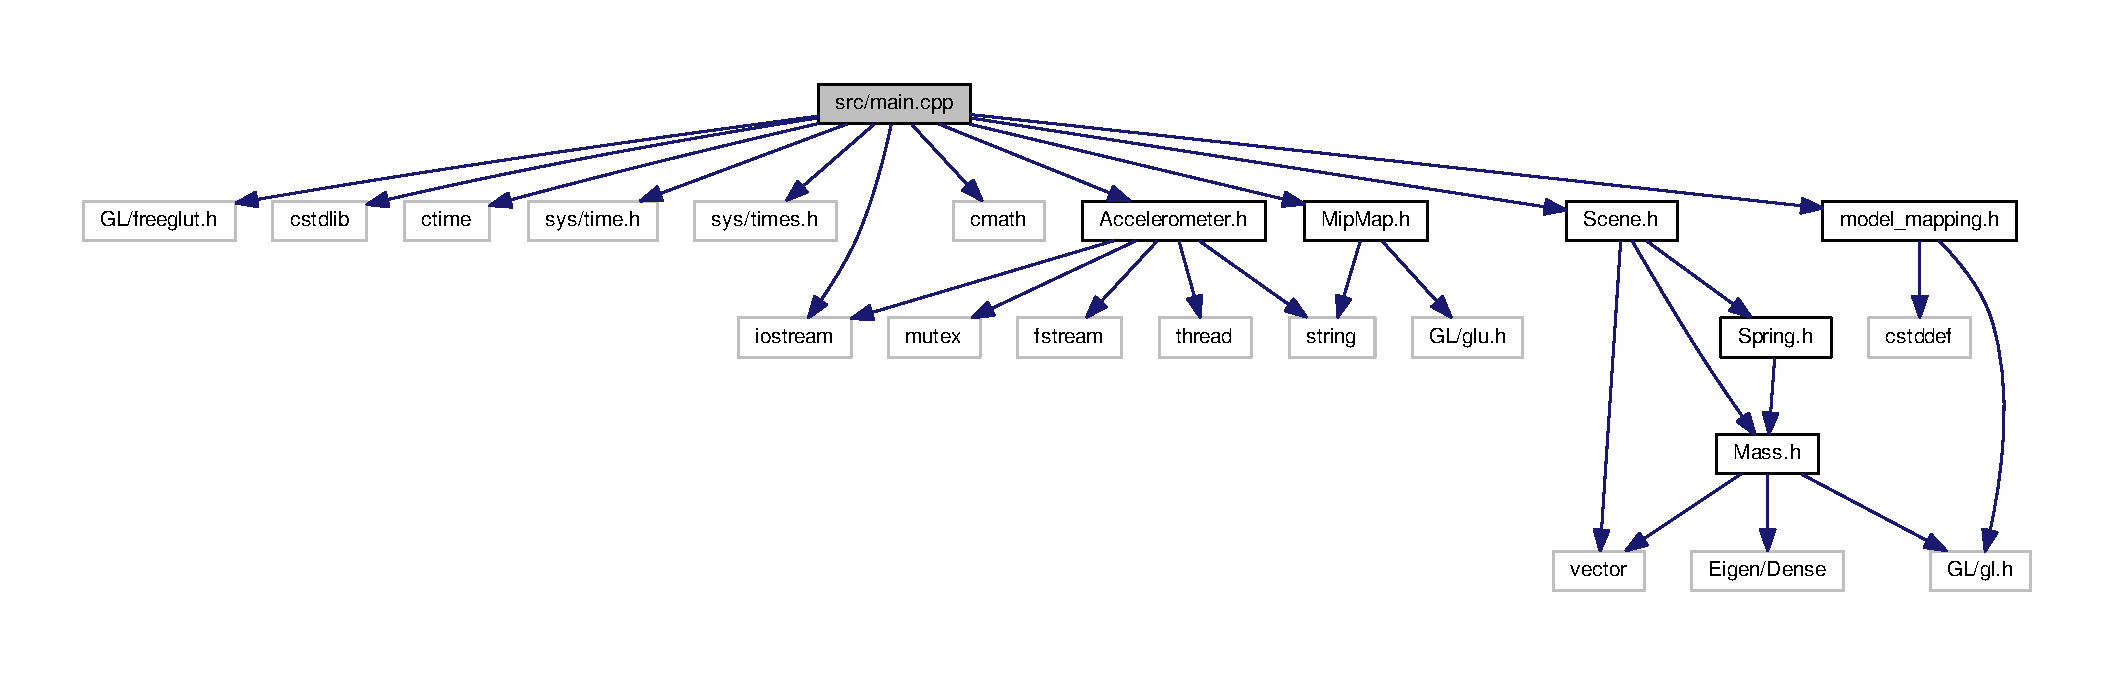
\includegraphics[width=350pt]{main_8cpp__incl}
\end{center}
\end{figure}
\subsection*{Functions}
\begin{DoxyCompactItemize}
\item 
ulong \hyperlink{main_8cpp_ae1c3ac19af566b079fd1d72cb8838fab}{get\+Time} ()
\item 
void \hyperlink{main_8cpp_a25a40b6614565f755233080a384c35f1}{initialize} ()
\item 
void \hyperlink{main_8cpp_a8a4b4b466e95577718229e81f137208a}{motion\+Callback} (int, int)
\item 
void \hyperlink{main_8cpp_afa25ae0e53443c4fa04ae9e93233aa78}{reshape\+Callback} (int w, int h)
\item 
void \hyperlink{main_8cpp_a582135b73e5577fe41fa9361870272b1}{update\+Simulation} ()
\item 
void \hyperlink{main_8cpp_a96162111a8d4ce79c3a93988682de9d4}{display\+Callback} ()
\item 
void \hyperlink{main_8cpp_a63650c4ea8c74f426870155b82a8ebad}{keyboard\+Callback} (unsigned char key, int, int)
\item 
void \hyperlink{main_8cpp_a11eb900902ba49145d19defcf4b164c0}{mouse\+Callback} (int button, int state, int x, int y)
\item 
void \hyperlink{main_8cpp_a3706e3b3d41de8ef254f10f16d415a7e}{idle\+Callback} ()
\item 
int \hyperlink{main_8cpp_a0ddf1224851353fc92bfbff6f499fa97}{main} (int argc, char $\ast$argv\mbox{[}$\,$\mbox{]})
\end{DoxyCompactItemize}
\subsection*{Variables}
\begin{DoxyCompactItemize}
\item 
\hyperlink{classstd_1_1Scene}{Scene} $\ast$ \hyperlink{main_8cpp_a6de66f9ad116ce1d596c7f4edc40c521}{scene} =nullptr
\item 
static const double \hyperlink{main_8cpp_ac1ad017c8f259a9a0a508ee9a6664229}{M\+A\+X\+\_\+\+U\+P\+D\+A\+T\+E\+\_\+\+T\+I\+M\+E} = 0.\+01
\end{DoxyCompactItemize}


\subsection{Function Documentation}
\hypertarget{main_8cpp_a96162111a8d4ce79c3a93988682de9d4}{}\index{main.\+cpp@{main.\+cpp}!display\+Callback@{display\+Callback}}
\index{display\+Callback@{display\+Callback}!main.\+cpp@{main.\+cpp}}
\subsubsection[{display\+Callback}]{\setlength{\rightskip}{0pt plus 5cm}void display\+Callback (
\begin{DoxyParamCaption}
{}
\end{DoxyParamCaption}
)}\label{main_8cpp_a96162111a8d4ce79c3a93988682de9d4}
Display callback function. Called each times the display needs to be redrawn. 

Here is the call graph for this function\+:\nopagebreak
\begin{figure}[H]
\begin{center}
\leavevmode
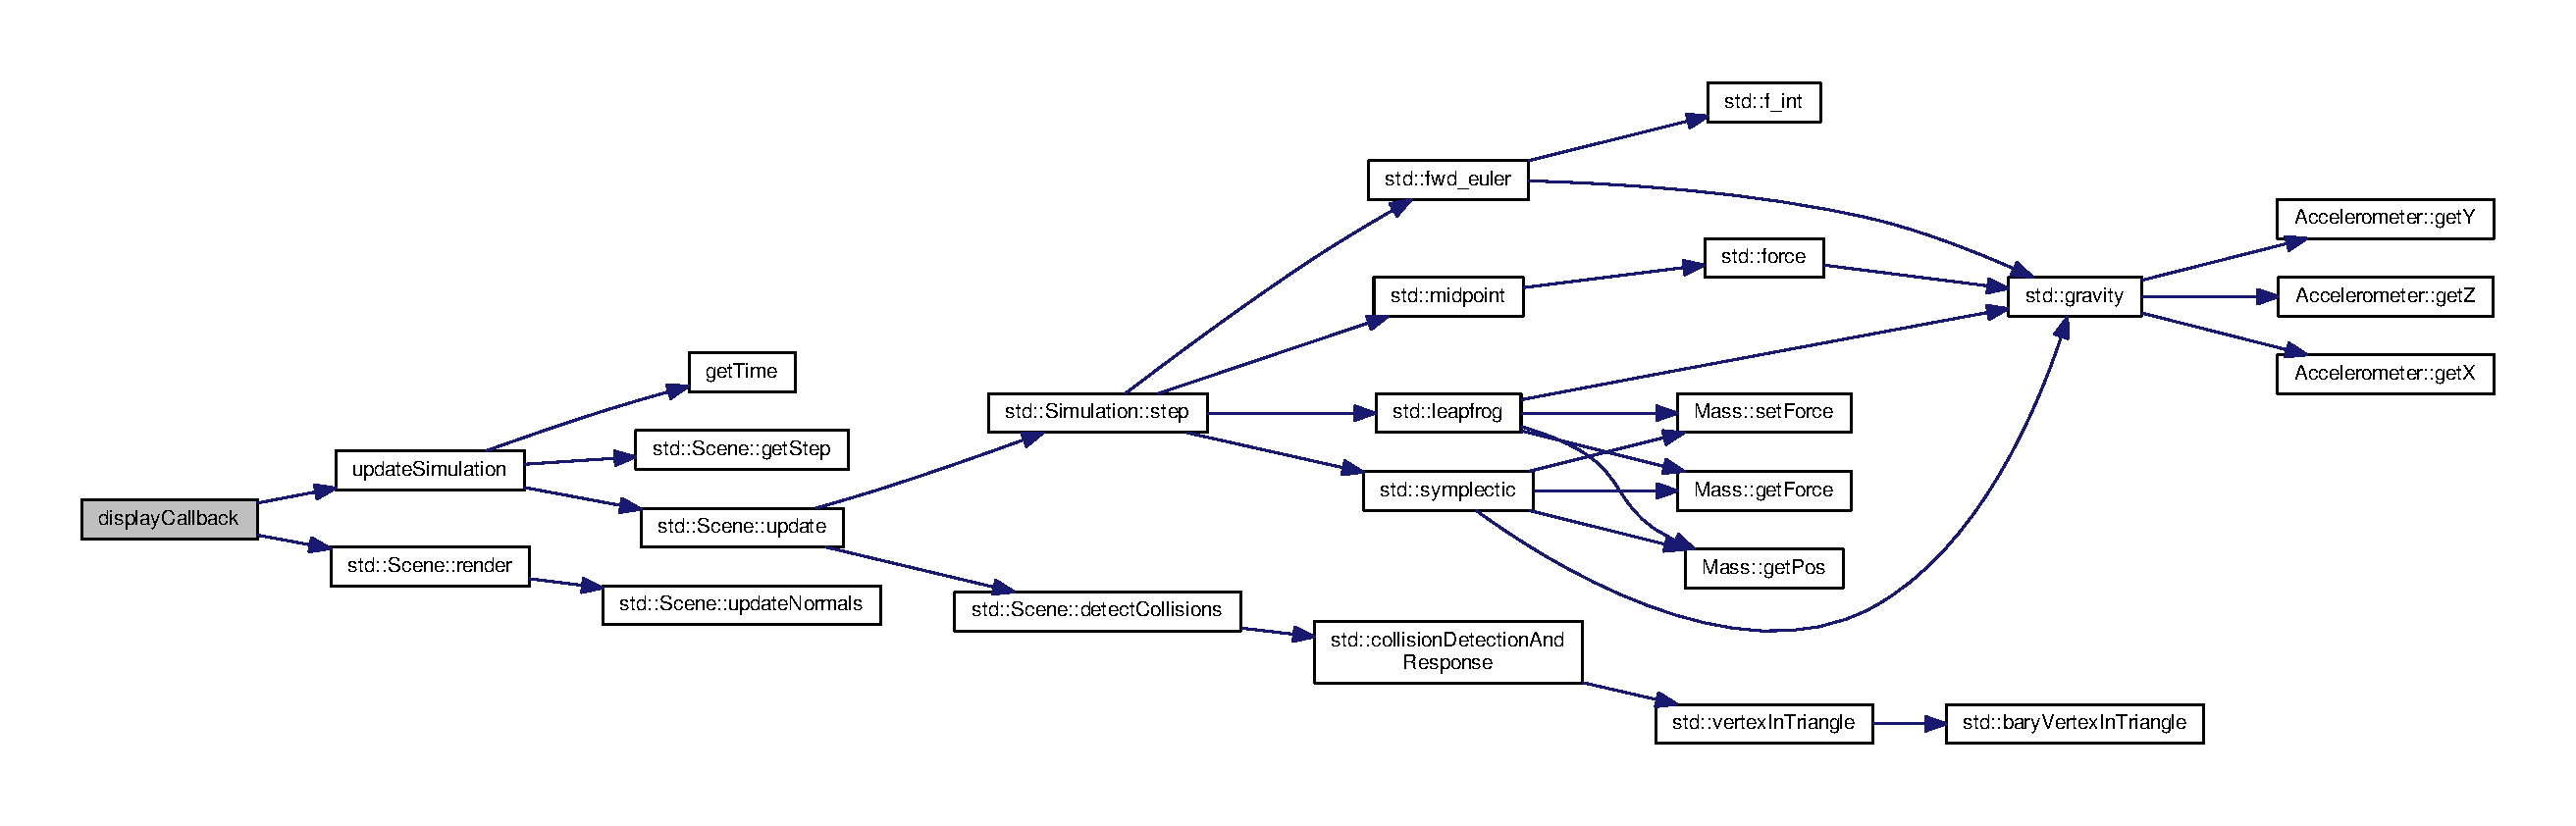
\includegraphics[width=350pt]{main_8cpp_a96162111a8d4ce79c3a93988682de9d4_cgraph}
\end{center}
\end{figure}


\hypertarget{main_8cpp_ae1c3ac19af566b079fd1d72cb8838fab}{}\index{main.\+cpp@{main.\+cpp}!get\+Time@{get\+Time}}
\index{get\+Time@{get\+Time}!main.\+cpp@{main.\+cpp}}
\subsubsection[{get\+Time}]{\setlength{\rightskip}{0pt plus 5cm}ulong get\+Time (
\begin{DoxyParamCaption}
{}
\end{DoxyParamCaption}
)}\label{main_8cpp_ae1c3ac19af566b079fd1d72cb8838fab}
Get the system time. This function requires $\ast$\+N\+I\+X dependent system functions. \begin{DoxyReturn}{Returns}
the time of now 
\end{DoxyReturn}
\hypertarget{main_8cpp_a3706e3b3d41de8ef254f10f16d415a7e}{}\index{main.\+cpp@{main.\+cpp}!idle\+Callback@{idle\+Callback}}
\index{idle\+Callback@{idle\+Callback}!main.\+cpp@{main.\+cpp}}
\subsubsection[{idle\+Callback}]{\setlength{\rightskip}{0pt plus 5cm}void idle\+Callback (
\begin{DoxyParamCaption}
{}
\end{DoxyParamCaption}
)}\label{main_8cpp_a3706e3b3d41de8ef254f10f16d415a7e}
Idle function. Executed if Open\+G\+L is in an idle state. \hypertarget{main_8cpp_a25a40b6614565f755233080a384c35f1}{}\index{main.\+cpp@{main.\+cpp}!initialize@{initialize}}
\index{initialize@{initialize}!main.\+cpp@{main.\+cpp}}
\subsubsection[{initialize}]{\setlength{\rightskip}{0pt plus 5cm}void initialize (
\begin{DoxyParamCaption}
{}
\end{DoxyParamCaption}
)}\label{main_8cpp_a25a40b6614565f755233080a384c35f1}
Initialize the Open\+G\+L system and the scene. 

Here is the call graph for this function\+:\nopagebreak
\begin{figure}[H]
\begin{center}
\leavevmode
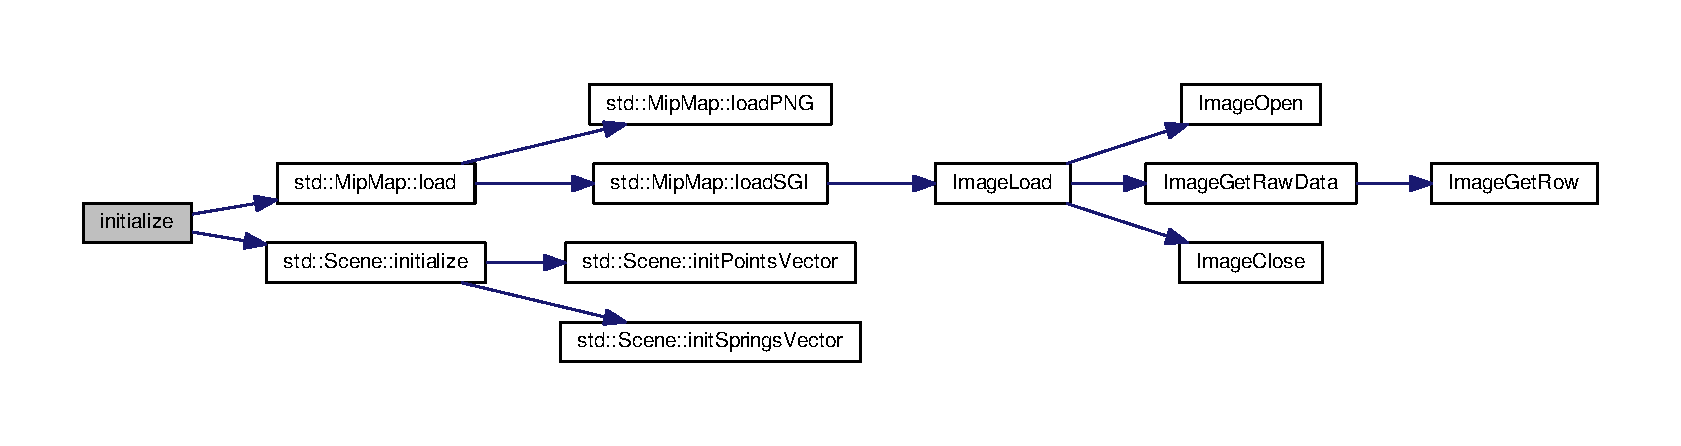
\includegraphics[width=350pt]{main_8cpp_a25a40b6614565f755233080a384c35f1_cgraph}
\end{center}
\end{figure}


\hypertarget{main_8cpp_a63650c4ea8c74f426870155b82a8ebad}{}\index{main.\+cpp@{main.\+cpp}!keyboard\+Callback@{keyboard\+Callback}}
\index{keyboard\+Callback@{keyboard\+Callback}!main.\+cpp@{main.\+cpp}}
\subsubsection[{keyboard\+Callback}]{\setlength{\rightskip}{0pt plus 5cm}void keyboard\+Callback (
\begin{DoxyParamCaption}
\item[{unsigned char}]{key, }
\item[{int}]{, }
\item[{int}]{}
\end{DoxyParamCaption}
)}\label{main_8cpp_a63650c4ea8c74f426870155b82a8ebad}
Keyboard callback function. Processes the input events from the keyboard. 
\begin{DoxyParams}{Parameters}
{\em key} & key mapped to an event \\
\hline
\end{DoxyParams}
\hypertarget{main_8cpp_a0ddf1224851353fc92bfbff6f499fa97}{}\index{main.\+cpp@{main.\+cpp}!main@{main}}
\index{main@{main}!main.\+cpp@{main.\+cpp}}
\subsubsection[{main}]{\setlength{\rightskip}{0pt plus 5cm}int main (
\begin{DoxyParamCaption}
\item[{int}]{argc, }
\item[{char $\ast$}]{argv\mbox{[}$\,$\mbox{]}}
\end{DoxyParamCaption}
)}\label{main_8cpp_a0ddf1224851353fc92bfbff6f499fa97}
The main function. 
\begin{DoxyParams}{Parameters}
{\em argc} & arguments counter. \\
\hline
{\em argv} & arguments vector. All arguments are passed on to {\ttfamily glut\+Init()} and {\ttfamily Scene()} \\
\hline
\end{DoxyParams}
\begin{DoxyReturn}{Returns}
process return value {\ttfamily E\+X\+I\+T\+\_\+\+S\+U\+C\+C\+E\+S\+S} or {\ttfamily E\+X\+I\+T\+\_\+\+F\+A\+I\+L\+U\+R\+E} 
\end{DoxyReturn}


Here is the call graph for this function\+:\nopagebreak
\begin{figure}[H]
\begin{center}
\leavevmode
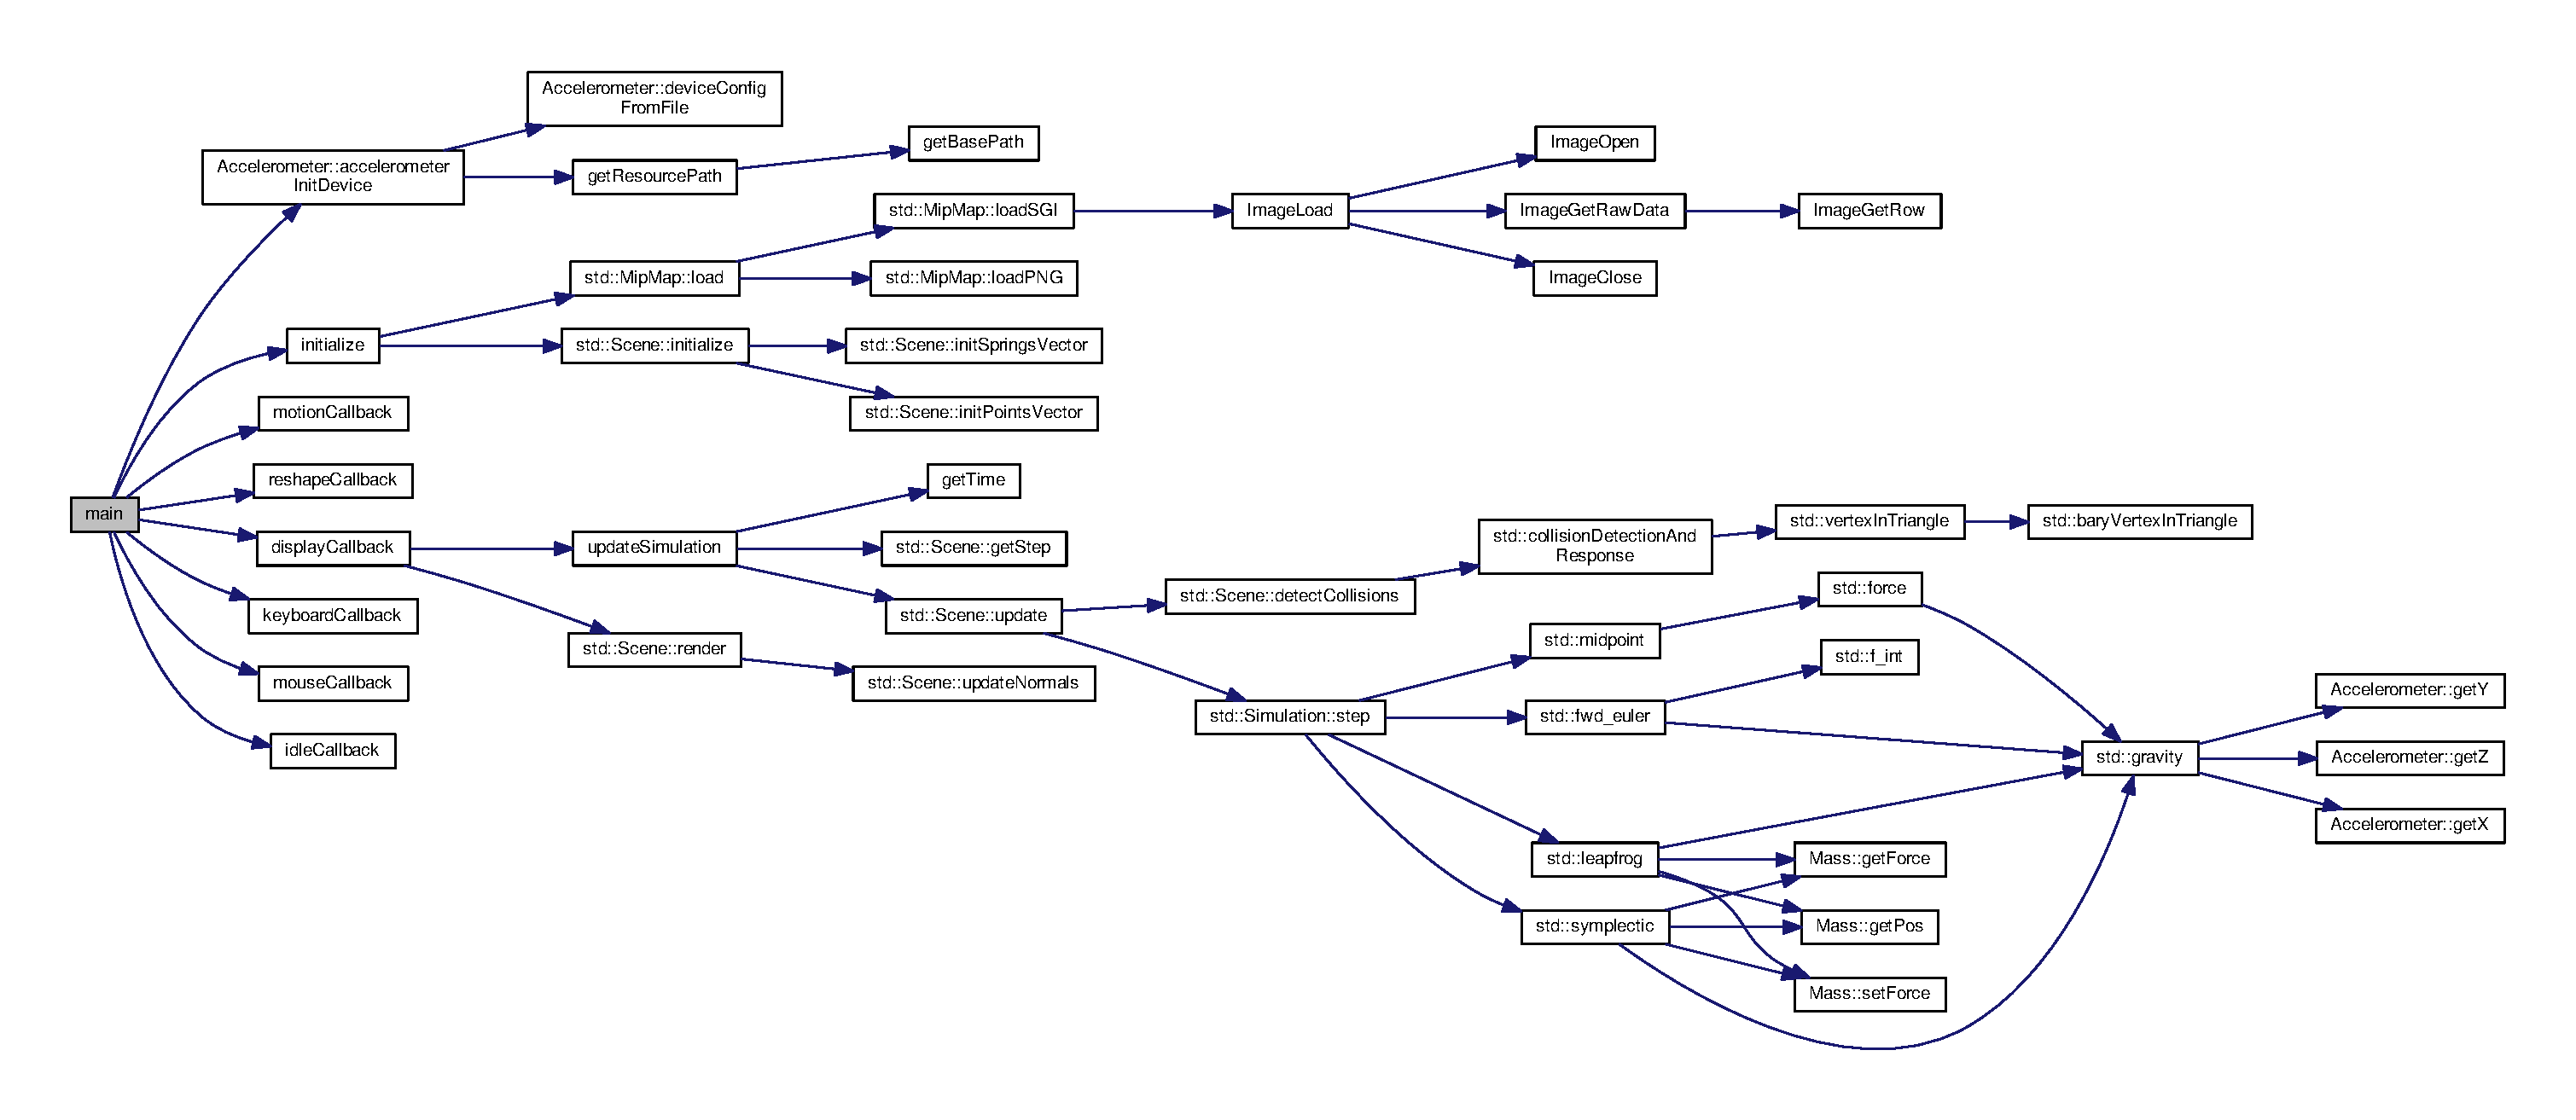
\includegraphics[width=350pt]{main_8cpp_a0ddf1224851353fc92bfbff6f499fa97_cgraph}
\end{center}
\end{figure}


\hypertarget{main_8cpp_a8a4b4b466e95577718229e81f137208a}{}\index{main.\+cpp@{main.\+cpp}!motion\+Callback@{motion\+Callback}}
\index{motion\+Callback@{motion\+Callback}!main.\+cpp@{main.\+cpp}}
\subsubsection[{motion\+Callback}]{\setlength{\rightskip}{0pt plus 5cm}void motion\+Callback (
\begin{DoxyParamCaption}
\item[{int}]{, }
\item[{int}]{}
\end{DoxyParamCaption}
)}\label{main_8cpp_a8a4b4b466e95577718229e81f137208a}
Mouse Motion callback function Processes the input events from the Mouse.

actually unused \hypertarget{main_8cpp_a11eb900902ba49145d19defcf4b164c0}{}\index{main.\+cpp@{main.\+cpp}!mouse\+Callback@{mouse\+Callback}}
\index{mouse\+Callback@{mouse\+Callback}!main.\+cpp@{main.\+cpp}}
\subsubsection[{mouse\+Callback}]{\setlength{\rightskip}{0pt plus 5cm}void mouse\+Callback (
\begin{DoxyParamCaption}
\item[{int}]{button, }
\item[{int}]{state, }
\item[{int}]{x, }
\item[{int}]{y}
\end{DoxyParamCaption}
)}\label{main_8cpp_a11eb900902ba49145d19defcf4b164c0}
Mouse button callback function. Processes the input events from the Mouse. 
\begin{DoxyParams}{Parameters}
{\em button} & \\
\hline
{\em state} & \\
\hline
{\em x} & \\
\hline
{\em y} & \\
\hline
\end{DoxyParams}
\hypertarget{main_8cpp_afa25ae0e53443c4fa04ae9e93233aa78}{}\index{main.\+cpp@{main.\+cpp}!reshape\+Callback@{reshape\+Callback}}
\index{reshape\+Callback@{reshape\+Callback}!main.\+cpp@{main.\+cpp}}
\subsubsection[{reshape\+Callback}]{\setlength{\rightskip}{0pt plus 5cm}void reshape\+Callback (
\begin{DoxyParamCaption}
\item[{int}]{w, }
\item[{int}]{h}
\end{DoxyParamCaption}
)}\label{main_8cpp_afa25ae0e53443c4fa04ae9e93233aa78}
Window reshape callback function. 
\begin{DoxyParams}{Parameters}
{\em w} & window width after size change \\
\hline
{\em h} & window height after size change \\
\hline
\end{DoxyParams}
\hypertarget{main_8cpp_a582135b73e5577fe41fa9361870272b1}{}\index{main.\+cpp@{main.\+cpp}!update\+Simulation@{update\+Simulation}}
\index{update\+Simulation@{update\+Simulation}!main.\+cpp@{main.\+cpp}}
\subsubsection[{update\+Simulation}]{\setlength{\rightskip}{0pt plus 5cm}void update\+Simulation (
\begin{DoxyParamCaption}
{}
\end{DoxyParamCaption}
)}\label{main_8cpp_a582135b73e5577fe41fa9361870272b1}
Update the simulation up to the present time. 

Here is the call graph for this function\+:\nopagebreak
\begin{figure}[H]
\begin{center}
\leavevmode
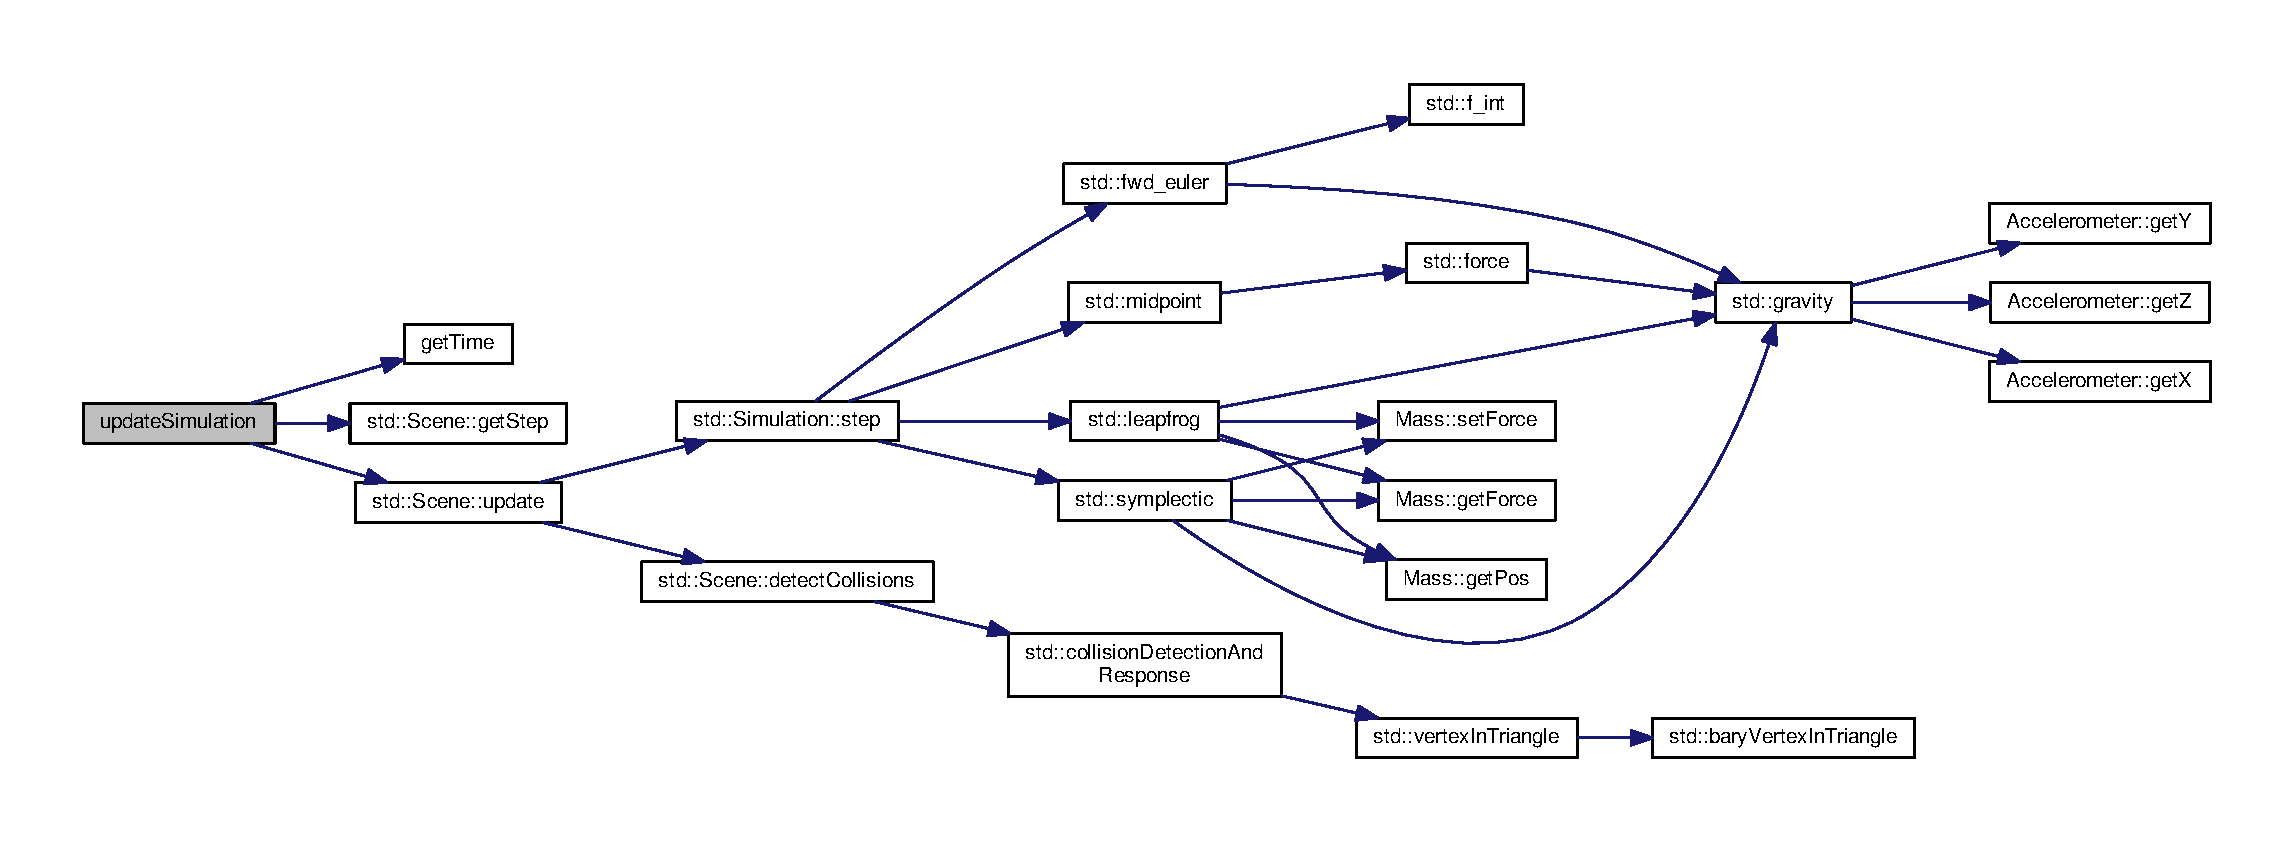
\includegraphics[width=350pt]{main_8cpp_a582135b73e5577fe41fa9361870272b1_cgraph}
\end{center}
\end{figure}




\subsection{Variable Documentation}
\hypertarget{main_8cpp_ac1ad017c8f259a9a0a508ee9a6664229}{}\index{main.\+cpp@{main.\+cpp}!M\+A\+X\+\_\+\+U\+P\+D\+A\+T\+E\+\_\+\+T\+I\+M\+E@{M\+A\+X\+\_\+\+U\+P\+D\+A\+T\+E\+\_\+\+T\+I\+M\+E}}
\index{M\+A\+X\+\_\+\+U\+P\+D\+A\+T\+E\+\_\+\+T\+I\+M\+E@{M\+A\+X\+\_\+\+U\+P\+D\+A\+T\+E\+\_\+\+T\+I\+M\+E}!main.\+cpp@{main.\+cpp}}
\subsubsection[{M\+A\+X\+\_\+\+U\+P\+D\+A\+T\+E\+\_\+\+T\+I\+M\+E}]{\setlength{\rightskip}{0pt plus 5cm}const double M\+A\+X\+\_\+\+U\+P\+D\+A\+T\+E\+\_\+\+T\+I\+M\+E = 0.\+01\hspace{0.3cm}{\ttfamily [static]}}\label{main_8cpp_ac1ad017c8f259a9a0a508ee9a6664229}
Maximum time allowed between updates when running in real-\/time mode (prevents performing too many calculations when running slower than real time) \hypertarget{main_8cpp_a6de66f9ad116ce1d596c7f4edc40c521}{}\index{main.\+cpp@{main.\+cpp}!scene@{scene}}
\index{scene@{scene}!main.\+cpp@{main.\+cpp}}
\subsubsection[{scene}]{\setlength{\rightskip}{0pt plus 5cm}{\bf Scene}$\ast$ scene =nullptr}\label{main_8cpp_a6de66f9ad116ce1d596c7f4edc40c521}

\hypertarget{Mass_8cpp}{}\section{src/\+Mass.cpp File Reference}
\label{Mass_8cpp}\index{src/\+Mass.\+cpp@{src/\+Mass.\+cpp}}
{\ttfamily \#include $<$G\+L/freeglut.\+h$>$}\\*
{\ttfamily \#include $<$vector$>$}\\*
{\ttfamily \#include \char`\"{}Mass.\+h\char`\"{}}\\*
{\ttfamily \#include \char`\"{}model\+\_\+mapping.\+h\char`\"{}}\\*
Include dependency graph for Mass.\+cpp\+:\nopagebreak
\begin{figure}[H]
\begin{center}
\leavevmode
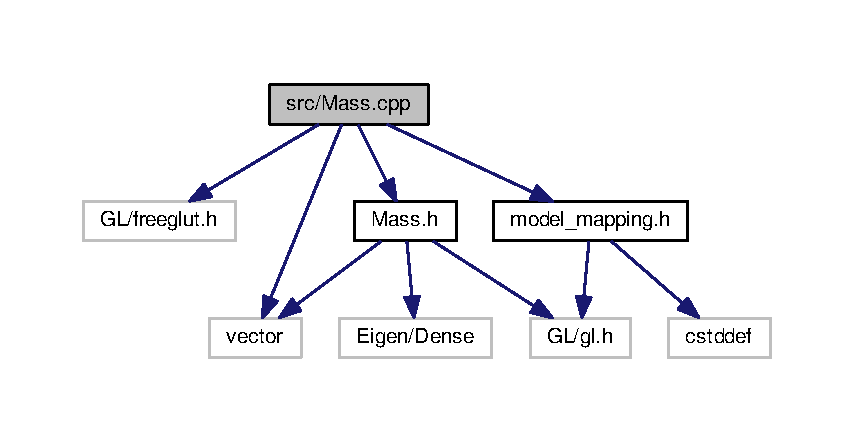
\includegraphics[width=350pt]{Mass_8cpp__incl}
\end{center}
\end{figure}
\subsection*{Macros}
\begin{DoxyCompactItemize}
\item 
\#define \hyperlink{Mass_8cpp_a11ab894ac45c63ab70f8f2758f370efe}{\+\_\+\+D\+E\+B\+U\+G\+\_\+\+M\+S\+G\+\_\+\+C}(X)
\item 
\#define \hyperlink{Mass_8cpp_a49190db5c55624c959dc898be8c10553}{\+\_\+\+D\+E\+B\+U\+G\+\_\+\+M\+S\+G}(X)
\end{DoxyCompactItemize}


\subsection{Macro Definition Documentation}
\hypertarget{Mass_8cpp_a49190db5c55624c959dc898be8c10553}{}\index{Mass.\+cpp@{Mass.\+cpp}!\+\_\+\+D\+E\+B\+U\+G\+\_\+\+M\+S\+G@{\+\_\+\+D\+E\+B\+U\+G\+\_\+\+M\+S\+G}}
\index{\+\_\+\+D\+E\+B\+U\+G\+\_\+\+M\+S\+G@{\+\_\+\+D\+E\+B\+U\+G\+\_\+\+M\+S\+G}!Mass.\+cpp@{Mass.\+cpp}}
\subsubsection[{\+\_\+\+D\+E\+B\+U\+G\+\_\+\+M\+S\+G}]{\setlength{\rightskip}{0pt plus 5cm}\#define \+\_\+\+D\+E\+B\+U\+G\+\_\+\+M\+S\+G(
\begin{DoxyParamCaption}
\item[{}]{X}
\end{DoxyParamCaption}
)}\label{Mass_8cpp_a49190db5c55624c959dc898be8c10553}
\hypertarget{Mass_8cpp_a11ab894ac45c63ab70f8f2758f370efe}{}\index{Mass.\+cpp@{Mass.\+cpp}!\+\_\+\+D\+E\+B\+U\+G\+\_\+\+M\+S\+G\+\_\+\+C@{\+\_\+\+D\+E\+B\+U\+G\+\_\+\+M\+S\+G\+\_\+\+C}}
\index{\+\_\+\+D\+E\+B\+U\+G\+\_\+\+M\+S\+G\+\_\+\+C@{\+\_\+\+D\+E\+B\+U\+G\+\_\+\+M\+S\+G\+\_\+\+C}!Mass.\+cpp@{Mass.\+cpp}}
\subsubsection[{\+\_\+\+D\+E\+B\+U\+G\+\_\+\+M\+S\+G\+\_\+\+C}]{\setlength{\rightskip}{0pt plus 5cm}\#define \+\_\+\+D\+E\+B\+U\+G\+\_\+\+M\+S\+G\+\_\+\+C(
\begin{DoxyParamCaption}
\item[{}]{X}
\end{DoxyParamCaption}
)}\label{Mass_8cpp_a11ab894ac45c63ab70f8f2758f370efe}

\hypertarget{Mass_8h}{}\section{src/\+Mass.h File Reference}
\label{Mass_8h}\index{src/\+Mass.\+h@{src/\+Mass.\+h}}
{\ttfamily \#include $<$G\+L/gl.\+h$>$}\\*
{\ttfamily \#include $<$Eigen/\+Dense$>$}\\*
{\ttfamily \#include $<$vector$>$}\\*
Include dependency graph for Mass.\+h\+:\nopagebreak
\begin{figure}[H]
\begin{center}
\leavevmode
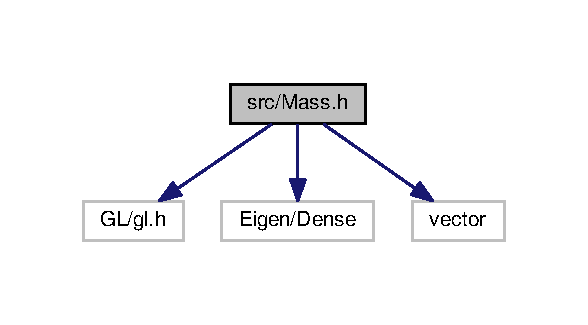
\includegraphics[width=282pt]{Mass_8h__incl}
\end{center}
\end{figure}
This graph shows which files directly or indirectly include this file\+:\nopagebreak
\begin{figure}[H]
\begin{center}
\leavevmode
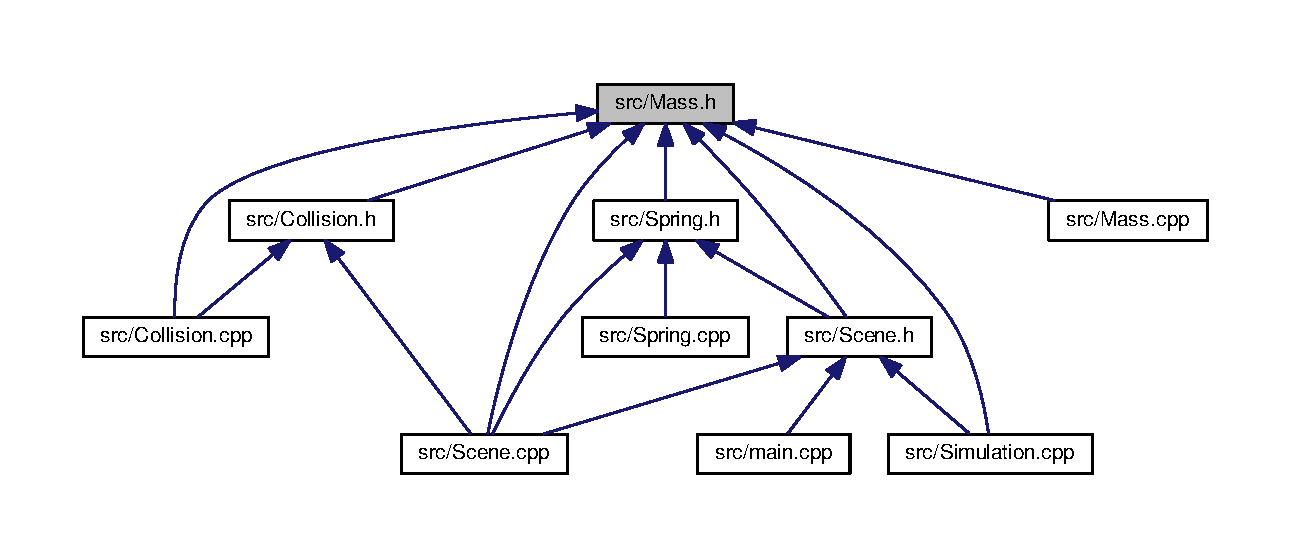
\includegraphics[width=350pt]{Mass_8h__dep__incl}
\end{center}
\end{figure}
\subsection*{Classes}
\begin{DoxyCompactItemize}
\item 
class \hyperlink{classMass}{Mass}
\end{DoxyCompactItemize}

\hypertarget{MipMap_8cpp}{}\section{src/\+Mip\+Map.cpp File Reference}
\label{MipMap_8cpp}\index{src/\+Mip\+Map.\+cpp@{src/\+Mip\+Map.\+cpp}}
{\ttfamily \#include \char`\"{}Mip\+Map.\+h\char`\"{}}\\*
{\ttfamily \#include $<$G\+L/glu.\+h$>$}\\*
{\ttfamily \#include $<$png.\+h$>$}\\*
{\ttfamily \#include $<$iostream$>$}\\*
{\ttfamily \#include \char`\"{}S\+G\+Iimage.\+h\char`\"{}}\\*
Include dependency graph for Mip\+Map.\+cpp\+:\nopagebreak
\begin{figure}[H]
\begin{center}
\leavevmode
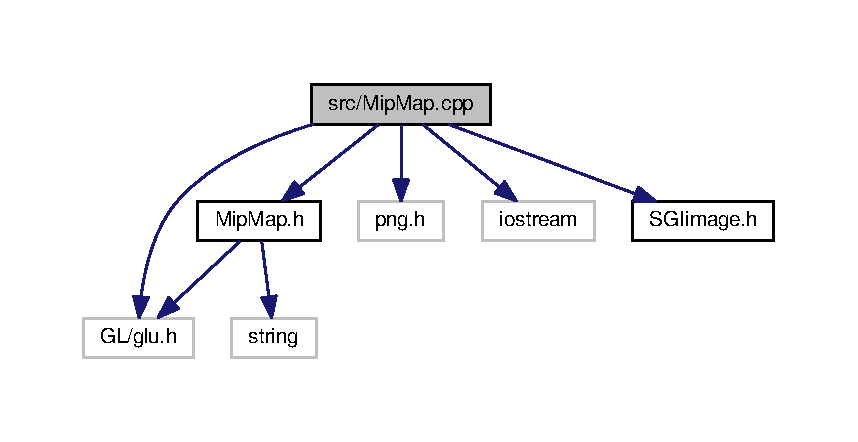
\includegraphics[width=350pt]{MipMap_8cpp__incl}
\end{center}
\end{figure}
\subsection*{Namespaces}
\begin{DoxyCompactItemize}
\item 
 \hyperlink{namespacestd}{std}
\end{DoxyCompactItemize}

\hypertarget{MipMap_8h}{}\section{src/\+Mip\+Map.h File Reference}
\label{MipMap_8h}\index{src/\+Mip\+Map.\+h@{src/\+Mip\+Map.\+h}}
{\ttfamily \#include $<$G\+L/glu.\+h$>$}\\*
{\ttfamily \#include $<$string$>$}\\*
Include dependency graph for Mip\+Map.\+h\+:\nopagebreak
\begin{figure}[H]
\begin{center}
\leavevmode
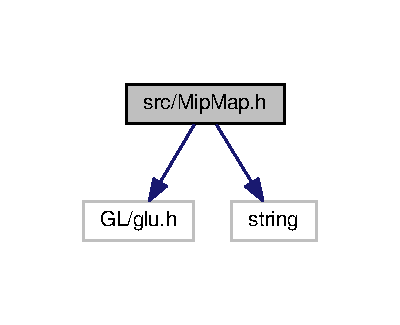
\includegraphics[width=192pt]{MipMap_8h__incl}
\end{center}
\end{figure}
This graph shows which files directly or indirectly include this file\+:\nopagebreak
\begin{figure}[H]
\begin{center}
\leavevmode
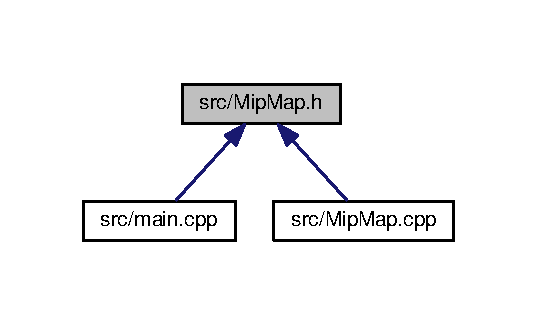
\includegraphics[width=258pt]{MipMap_8h__dep__incl}
\end{center}
\end{figure}
\subsection*{Classes}
\begin{DoxyCompactItemize}
\item 
class \hyperlink{classstd_1_1MipMap}{std\+::\+Mip\+Map}
\end{DoxyCompactItemize}
\subsection*{Namespaces}
\begin{DoxyCompactItemize}
\item 
 \hyperlink{namespacestd}{std}
\end{DoxyCompactItemize}

\hypertarget{model__mapping_8cpp}{}\section{src/model\+\_\+mapping.cpp File Reference}
\label{model__mapping_8cpp}\index{src/model\+\_\+mapping.\+cpp@{src/model\+\_\+mapping.\+cpp}}
{\ttfamily \#include $<$G\+L/gl.\+h$>$}\\*
{\ttfamily \#include $<$cstddef$>$}\\*
{\ttfamily \#include \char`\"{}model\+\_\+mapping.\+h\char`\"{}}\\*
{\ttfamily \#include \char`\"{}skirt\+\_\+sphere.\+h\char`\"{}}\\*
Include dependency graph for model\+\_\+mapping.\+cpp\+:\nopagebreak
\begin{figure}[H]
\begin{center}
\leavevmode
\includegraphics[width=323pt]{model__mapping_8cpp__incl}
\end{center}
\end{figure}
\subsection*{Namespaces}
\begin{DoxyCompactItemize}
\item 
 \hyperlink{namespacestd}{std}
\end{DoxyCompactItemize}
\subsection*{Macros}
\begin{DoxyCompactItemize}
\item 
\#define \hyperlink{model__mapping_8cpp_a4d1624dd68db4a8494c5e998b5aa60f9}{M\+O\+D\+E\+L}(X)~skirt\+\_\+sphere\#\#X
\end{DoxyCompactItemize}
\subsection*{Variables}
\begin{DoxyCompactItemize}
\item 
const size\+\_\+t \hyperlink{namespacestd_a2c56d5934d3e2877598b1eba9302a70f}{std\+::model3d\+Vertices} = \hyperlink{model__mapping_8cpp_a4d1624dd68db4a8494c5e998b5aa60f9}{M\+O\+D\+E\+L}(Vertices)
\begin{DoxyCompactList}\small\item\em number of vertices \end{DoxyCompactList}\item 
G\+Lfloat $\ast$ \hyperlink{namespacestd_aa45ed5de4e82f7ca1e4fd453a157715c}{std\+::model3d\+Positions} = \hyperlink{model__mapping_8cpp_a4d1624dd68db4a8494c5e998b5aa60f9}{M\+O\+D\+E\+L}(Positions)
\begin{DoxyCompactList}\small\item\em all vertex positions \end{DoxyCompactList}\item 
G\+Lfloat $\ast$ \hyperlink{namespacestd_a75a224804224819d960875bd982ce0c6}{std\+::model3d\+Texels} = \hyperlink{model__mapping_8cpp_a4d1624dd68db4a8494c5e998b5aa60f9}{M\+O\+D\+E\+L}(Texels)
\begin{DoxyCompactList}\small\item\em all texture coordinates \end{DoxyCompactList}\item 
G\+Lfloat $\ast$ \hyperlink{namespacestd_ab62b34140cca60f41eac455edd195e5a}{std\+::model3d\+Normals} = \hyperlink{model__mapping_8cpp_a4d1624dd68db4a8494c5e998b5aa60f9}{M\+O\+D\+E\+L}(Normals)
\begin{DoxyCompactList}\small\item\em all normals of the face surfaces \end{DoxyCompactList}\item 
const size\+\_\+t \hyperlink{namespacestd_a74aad4fa6e8a984849221081da2ef691}{std\+::model3d\+Objects\+With\+Mass} = \hyperlink{model__mapping_8cpp_a4d1624dd68db4a8494c5e998b5aa60f9}{M\+O\+D\+E\+L}(Objects\+With\+Mass)
\begin{DoxyCompactList}\small\item\em number of objects to apply to the mass-\/spring simulation \end{DoxyCompactList}\item 
const size\+\_\+t $\ast$ \hyperlink{namespacestd_a20a6e87f65453b04a7eac93004989039}{std\+::model3d\+Masses} = \hyperlink{model__mapping_8cpp_a4d1624dd68db4a8494c5e998b5aa60f9}{M\+O\+D\+E\+L}(Masses)
\begin{DoxyCompactList}\small\item\em array of 3\+D-\/objects with mass \end{DoxyCompactList}\item 
const size\+\_\+t $\ast$ \hyperlink{namespacestd_a22dba9fb8da88b07cd8b471827b6fac7}{std\+::model3d\+Mass\+Fwd\+Offs} = \hyperlink{model__mapping_8cpp_a4d1624dd68db4a8494c5e998b5aa60f9}{M\+O\+D\+E\+L}(Mass\+Fwd\+Offs)
\begin{DoxyCompactList}\small\item\em offset in the points array \end{DoxyCompactList}\item 
const size\+\_\+t $\ast$ \hyperlink{namespacestd_aea2c80cb8809cdc4c2f3b2b0961d3036}{std\+::model3d\+Mass\+Vertices} = \hyperlink{model__mapping_8cpp_a4d1624dd68db4a8494c5e998b5aa60f9}{M\+O\+D\+E\+L}(Mass\+Vertices)
\begin{DoxyCompactList}\small\item\em number of vertices per object with mass \end{DoxyCompactList}\item 
const size\+\_\+t $\ast$ \hyperlink{namespacestd_acb567e43ad7c5a09fec7eeed5b529d96}{std\+::model3d\+Mass\+Rev\+Offs} = \hyperlink{model__mapping_8cpp_a4d1624dd68db4a8494c5e998b5aa60f9}{M\+O\+D\+E\+L}(Mass\+Rev\+Offs)
\begin{DoxyCompactList}\small\item\em offsets for the model3d\+Rev\+Index array \end{DoxyCompactList}\item 
const size\+\_\+t $\ast$ \hyperlink{namespacestd_ad0535524d79ce742b34e78404e55a224}{std\+::model3d\+Mass\+Rev\+Offs\+Orig} = \hyperlink{model__mapping_8cpp_a4d1624dd68db4a8494c5e998b5aa60f9}{M\+O\+D\+E\+L}(Mass\+Rev\+Offs\+Orig)
\begin{DoxyCompactList}\small\item\em offset to the first vertex of an object with mass \end{DoxyCompactList}\item 
const size\+\_\+t $\ast$$\ast$ \hyperlink{namespacestd_a339638085d29cb13db371a07634085c6}{std\+::model3d\+Fwd\+Index} = \hyperlink{model__mapping_8cpp_a4d1624dd68db4a8494c5e998b5aa60f9}{M\+O\+D\+E\+L}(Fwd\+Index)
\begin{DoxyCompactList}\small\item\em indices of the mass-\/points in the positions array \end{DoxyCompactList}\item 
const size\+\_\+t $\ast$ \hyperlink{namespacestd_a0ff16d332f71a0822fb8570c16df06ff}{std\+::model3d\+Fwd\+Index\+Length} = \hyperlink{model__mapping_8cpp_a4d1624dd68db4a8494c5e998b5aa60f9}{M\+O\+D\+E\+L}(Fwd\+Index\+Length)
\begin{DoxyCompactList}\small\item\em number of indices for each mass-\/point \end{DoxyCompactList}\item 
const size\+\_\+t $\ast$ \hyperlink{namespacestd_a13dd980059224bfd90cd1fde9aa706a9}{std\+::model3d\+Rev\+Index} = \hyperlink{model__mapping_8cpp_a4d1624dd68db4a8494c5e998b5aa60f9}{M\+O\+D\+E\+L}(Rev\+Index)
\begin{DoxyCompactList}\small\item\em index of a vertex in the mass-\/points array \end{DoxyCompactList}\item 
const size\+\_\+t \hyperlink{namespacestd_ae8e9077260287353aa87ecaadb67b8e7}{std\+::model3d\+Objects} = \hyperlink{model__mapping_8cpp_a4d1624dd68db4a8494c5e998b5aa60f9}{M\+O\+D\+E\+L}(Objects)
\begin{DoxyCompactList}\small\item\em number of 3\+D-\/objects \end{DoxyCompactList}\item 
const size\+\_\+t $\ast$ \hyperlink{namespacestd_a34c26b88877b9e50d420b2f5ee1c1c47}{std\+::model3d\+Object\+Offset} = \hyperlink{model__mapping_8cpp_a4d1624dd68db4a8494c5e998b5aa60f9}{M\+O\+D\+E\+L}(Object\+Offset)
\begin{DoxyCompactList}\small\item\em offset to the first vertex of a 3\+D-\/object \end{DoxyCompactList}\item 
const size\+\_\+t $\ast$ \hyperlink{namespacestd_a678ef71cdf9ee666493694bfcf4d238f}{std\+::model3d\+Object\+Length} = \hyperlink{model__mapping_8cpp_a4d1624dd68db4a8494c5e998b5aa60f9}{M\+O\+D\+E\+L}(Object\+Length)
\begin{DoxyCompactList}\small\item\em number of vertices for each 3\+D-\/object \end{DoxyCompactList}\item 
const char $\ast$$\ast$ \hyperlink{namespacestd_af3ac1c474abd23473b8fca32585ffe52}{std\+::model3d\+Object\+Names} = (const char$\ast$$\ast$) \hyperlink{model__mapping_8cpp_a4d1624dd68db4a8494c5e998b5aa60f9}{M\+O\+D\+E\+L}(Object\+Names)
\begin{DoxyCompactList}\small\item\em names of the objects (for identification) \end{DoxyCompactList}\item 
const char $\ast$ \hyperlink{namespacestd_ab193fa08b6666c1bca6ccbb53acd58f6}{std\+::model3d\+Texture\+File\+Path} = \char`\"{}textures/textures\+\_\+all.\+rgb\char`\"{}
\begin{DoxyCompactList}\small\item\em path to the texture-\/image file \end{DoxyCompactList}\end{DoxyCompactItemize}


\subsection{Detailed Description}
This file includes the vertex, texture and normals coordinates and some 3\+D object topology informations.

It is a wrapper to make the code relying on these variables independent from varying names supplied by the header file generator tool {\ttfamily blender2o\+G\+L}. Use the following line to generate a customized header file\+: 
\begin{DoxyCode}
blender2oGL ./path/to-your/file.obj -m -s -o -r -a file\_objectWithMass -a file\_otherObjectIfDesired
\end{DoxyCode}
 Edit the pointers in this file to fit the code to an exchanged header file. D\+O\+N\textquotesingle{}T E\+D\+I\+T them in the generated .h file, they may be overwritten by the generator tool. 

\subsection{Macro Definition Documentation}
\hypertarget{model__mapping_8cpp_a4d1624dd68db4a8494c5e998b5aa60f9}{}\index{model\+\_\+mapping.\+cpp@{model\+\_\+mapping.\+cpp}!M\+O\+D\+E\+L@{M\+O\+D\+E\+L}}
\index{M\+O\+D\+E\+L@{M\+O\+D\+E\+L}!model\+\_\+mapping.\+cpp@{model\+\_\+mapping.\+cpp}}
\subsubsection[{M\+O\+D\+E\+L}]{\setlength{\rightskip}{0pt plus 5cm}\#define M\+O\+D\+E\+L(
\begin{DoxyParamCaption}
\item[{}]{X}
\end{DoxyParamCaption}
)~skirt\+\_\+sphere\#\#X}\label{model__mapping_8cpp_a4d1624dd68db4a8494c5e998b5aa60f9}
define the prefix of the structures for mapping the variable names 
\hypertarget{model__mapping_8h}{}\section{src/model\+\_\+mapping.h File Reference}
\label{model__mapping_8h}\index{src/model\+\_\+mapping.\+h@{src/model\+\_\+mapping.\+h}}
{\ttfamily \#include $<$G\+L/gl.\+h$>$}\\*
{\ttfamily \#include $<$cstddef$>$}\\*
Include dependency graph for model\+\_\+mapping.\+h\+:\nopagebreak
\begin{figure}[H]
\begin{center}
\leavevmode
\includegraphics[width=196pt]{model__mapping_8h__incl}
\end{center}
\end{figure}
This graph shows which files directly or indirectly include this file\+:\nopagebreak
\begin{figure}[H]
\begin{center}
\leavevmode
\includegraphics[width=350pt]{model__mapping_8h__dep__incl}
\end{center}
\end{figure}
\subsection*{Namespaces}
\begin{DoxyCompactItemize}
\item 
 \hyperlink{namespacestd}{std}
\end{DoxyCompactItemize}


\subsection{Detailed Description}
This file includes the vertex, texture and normals coordinates and some 3\+D object topology informations.

It is a wrapper to make the code relying on these variables independent from varying names supplied by the header file generator tool \textquotesingle{}blender2o\+G\+L\textquotesingle{}

Edit the pointers in the \textquotesingle{}\hyperlink{model__mapping_8cpp}{model\+\_\+mapping.\+cpp}\textquotesingle{} file to fit the code to an exchanged header file. D\+O\+N\textquotesingle{}T E\+D\+I\+T them in the generated .h file, they may be overwritten by the generator tool.

See \textquotesingle{}\hyperlink{model__mapping_8cpp}{model\+\_\+mapping.\+cpp}\textquotesingle{} for further details. 
\hypertarget{ResourcePath_8h}{}\section{src/\+Resource\+Path.h File Reference}
\label{ResourcePath_8h}\index{src/\+Resource\+Path.\+h@{src/\+Resource\+Path.\+h}}
{\ttfamily \#include $<$iostream$>$}\\*
{\ttfamily \#include $<$string$>$}\\*
Include dependency graph for Resource\+Path.\+h\+:\nopagebreak
\begin{figure}[H]
\begin{center}
\leavevmode
\includegraphics[width=194pt]{ResourcePath_8h__incl}
\end{center}
\end{figure}
This graph shows which files directly or indirectly include this file\+:\nopagebreak
\begin{figure}[H]
\begin{center}
\leavevmode
\includegraphics[width=195pt]{ResourcePath_8h__dep__incl}
\end{center}
\end{figure}
\subsection*{Functions}
\begin{DoxyCompactItemize}
\item 
string \hyperlink{ResourcePath_8h_a49c5dd4204aaeea4802d8fa9d7c8fccc}{get\+Base\+Path} (int, char $\ast$argv\mbox{[}$\,$\mbox{]}=nullptr)
\begin{DoxyCompactList}\small\item\em Get the path of the application folder. \end{DoxyCompactList}\item 
string \hyperlink{ResourcePath_8h_ac072528545a90c4040a7b43c161a8e5a}{get\+Resource\+Path} (string file\+Path, string resources\+Folder=\char`\"{}resources\char`\"{}, int argc=0, char $\ast$argv\mbox{[}$\,$\mbox{]}=nullptr)
\begin{DoxyCompactList}\small\item\em Get path to resource file relative to the Base\+Path(). \end{DoxyCompactList}\end{DoxyCompactItemize}


\subsection{Function Documentation}
\hypertarget{ResourcePath_8h_a49c5dd4204aaeea4802d8fa9d7c8fccc}{}\index{Resource\+Path.\+h@{Resource\+Path.\+h}!get\+Base\+Path@{get\+Base\+Path}}
\index{get\+Base\+Path@{get\+Base\+Path}!Resource\+Path.\+h@{Resource\+Path.\+h}}
\subsubsection[{get\+Base\+Path}]{\setlength{\rightskip}{0pt plus 5cm}string get\+Base\+Path (
\begin{DoxyParamCaption}
\item[{int}]{, }
\item[{char $\ast$}]{argv\mbox{[}$\,$\mbox{]} = {\ttfamily nullptr}}
\end{DoxyParamCaption}
)}\label{ResourcePath_8h_a49c5dd4204aaeea4802d8fa9d7c8fccc}


Get the path of the application folder. 

The path returned is an absolute path with trailing path separator. The first call of this function initializes the path constant and thus, it needs non-\/null values for argc and argv. If the initialization fails, the return value is an empty string.


\begin{DoxyParams}{Parameters}
{\em argv} & the arguments list provided by the {\ttfamily \hyperlink{main_8cpp_a0ddf1224851353fc92bfbff6f499fa97}{main()}} function on first call, omit or set to {\ttfamily nullptr} on succeeding calls \\
\hline
\end{DoxyParams}
\begin{DoxyReturn}{Returns}
the base path or an empty string if not initialized. 
\end{DoxyReturn}
\hypertarget{ResourcePath_8h_ac072528545a90c4040a7b43c161a8e5a}{}\index{Resource\+Path.\+h@{Resource\+Path.\+h}!get\+Resource\+Path@{get\+Resource\+Path}}
\index{get\+Resource\+Path@{get\+Resource\+Path}!Resource\+Path.\+h@{Resource\+Path.\+h}}
\subsubsection[{get\+Resource\+Path}]{\setlength{\rightskip}{0pt plus 5cm}string get\+Resource\+Path (
\begin{DoxyParamCaption}
\item[{string}]{file\+Path, }
\item[{string}]{resources\+Folder = {\ttfamily \char`\"{}resources\char`\"{}}, }
\item[{int}]{argc = {\ttfamily 0}, }
\item[{char $\ast$}]{argv\mbox{[}$\,$\mbox{]} = {\ttfamily nullptr}}
\end{DoxyParamCaption}
)}\label{ResourcePath_8h_ac072528545a90c4040a7b43c161a8e5a}


Get path to resource file relative to the Base\+Path(). 

The path returned is an absolute path resolved from ../resources/file\+Path. If the path to a sub-\/folder is required use the path separator supported by the target system. 
\begin{DoxyParams}{Parameters}
{\em file\+Path} & the path to the requested file in the resources folder \\
\hline
{\em resources\+Folder} & name of the folder without path separators or empty string to address the parent folder, default is \char`\"{}resources\char`\"{} \\
\hline
{\em argc} & the arguments count of the {\ttfamily \hyperlink{main_8cpp_a0ddf1224851353fc92bfbff6f499fa97}{main()}} function on first call \\
\hline
{\em argv} & the arguments list of the {\ttfamily \hyperlink{main_8cpp_a0ddf1224851353fc92bfbff6f499fa97}{main()}} function on first call \\
\hline
\end{DoxyParams}
\begin{DoxyReturn}{Returns}
the base path to the resource folder appended by file\+Path 
\end{DoxyReturn}


Here is the call graph for this function\+:\nopagebreak
\begin{figure}[H]
\begin{center}
\leavevmode
\includegraphics[width=281pt]{ResourcePath_8h_ac072528545a90c4040a7b43c161a8e5a_cgraph}
\end{center}
\end{figure}



\hypertarget{Scene_8cpp}{}\section{src/\+Scene.cpp File Reference}
\label{Scene_8cpp}\index{src/\+Scene.\+cpp@{src/\+Scene.\+cpp}}
{\ttfamily \#include $<$G\+L/freeglut.\+h$>$}\\*
{\ttfamily \#include $<$cstring$>$}\\*
{\ttfamily \#include $<$cstdlib$>$}\\*
{\ttfamily \#include $<$iostream$>$}\\*
{\ttfamily \#include $<$Eigen/\+Dense$>$}\\*
{\ttfamily \#include $<$Eigen/\+Geometry$>$}\\*
{\ttfamily \#include \char`\"{}Scene.\+h\char`\"{}}\\*
{\ttfamily \#include \char`\"{}Mass.\+h\char`\"{}}\\*
{\ttfamily \#include \char`\"{}Spring.\+h\char`\"{}}\\*
{\ttfamily \#include \char`\"{}Simulation.\+h\char`\"{}}\\*
{\ttfamily \#include \char`\"{}Collision.\+h\char`\"{}}\\*
{\ttfamily \#include \char`\"{}model\+\_\+mapping.\+h\char`\"{}}\\*
Include dependency graph for Scene.\+cpp\+:\nopagebreak
\begin{figure}[H]
\begin{center}
\leavevmode
\includegraphics[width=350pt]{Scene_8cpp__incl}
\end{center}
\end{figure}
\subsection*{Namespaces}
\begin{DoxyCompactItemize}
\item 
 \hyperlink{namespacestd}{std}
\end{DoxyCompactItemize}

\hypertarget{Scene_8h}{}\section{src/\+Scene.h File Reference}
\label{Scene_8h}\index{src/\+Scene.\+h@{src/\+Scene.\+h}}
{\ttfamily \#include $<$vector$>$}\\*
{\ttfamily \#include \char`\"{}Mass.\+h\char`\"{}}\\*
{\ttfamily \#include \char`\"{}Spring.\+h\char`\"{}}\\*
Include dependency graph for Scene.\+h\+:\nopagebreak
\begin{figure}[H]
\begin{center}
\leavevmode
\includegraphics[width=282pt]{Scene_8h__incl}
\end{center}
\end{figure}
This graph shows which files directly or indirectly include this file\+:\nopagebreak
\begin{figure}[H]
\begin{center}
\leavevmode
\includegraphics[width=350pt]{Scene_8h__dep__incl}
\end{center}
\end{figure}
\subsection*{Classes}
\begin{DoxyCompactItemize}
\item 
class \hyperlink{classstd_1_1Scene}{std\+::\+Scene}
\end{DoxyCompactItemize}
\subsection*{Namespaces}
\begin{DoxyCompactItemize}
\item 
 \hyperlink{namespacestd}{std}
\end{DoxyCompactItemize}

\hypertarget{SGIimage_8c}{}\section{src/\+S\+G\+Iimage.c File Reference}
\label{SGIimage_8c}\index{src/\+S\+G\+Iimage.\+c@{src/\+S\+G\+Iimage.\+c}}
{\ttfamily \#include $<$stdio.\+h$>$}\\*
{\ttfamily \#include $<$stdlib.\+h$>$}\\*
{\ttfamily \#include \char`\"{}S\+G\+Iimage.\+h\char`\"{}}\\*
Include dependency graph for S\+G\+Iimage.\+c\+:\nopagebreak
\begin{figure}[H]
\begin{center}
\leavevmode
\includegraphics[width=278pt]{SGIimage_8c__incl}
\end{center}
\end{figure}
\subsection*{Classes}
\begin{DoxyCompactItemize}
\item 
struct \hyperlink{structImage}{Image}
\end{DoxyCompactItemize}
\subsection*{Macros}
\begin{DoxyCompactItemize}
\item 
\#define \hyperlink{SGIimage_8c_ae85edbe538f26e9d7c01ce9575e5a869}{I\+M\+A\+G\+I\+C}~0x01da
\item 
\#define \hyperlink{SGIimage_8c_abb38fb3b165149d6f89182858a0a69a8}{I\+M\+A\+G\+I\+C\+\_\+\+S\+W\+A\+P}~0xda01
\item 
\#define \hyperlink{SGIimage_8c_a7d328a88b3bb666030687fedff1c1731}{S\+W\+A\+P\+\_\+\+S\+H\+O\+R\+T\+\_\+\+B\+Y\+T\+E\+S}(x)~((((x) \& 0xff) $<$$<$ 8) $\vert$ (((x) \& 0xff00) $>$$>$ 8))
\item 
\#define \hyperlink{SGIimage_8c_aeb2cd9336afe0983ef5bcf18088bd05d}{S\+W\+A\+P\+\_\+\+L\+O\+N\+G\+\_\+\+B\+Y\+T\+E\+S}(x)
\end{DoxyCompactItemize}
\subsection*{Functions}
\begin{DoxyCompactItemize}
\item 
static \hyperlink{structImage}{Image} $\ast$ \hyperlink{SGIimage_8c_a3967a181b57e2a65499de032d78157cc}{Image\+Open} (char $\ast$file\+Name)
\item 
static void \hyperlink{SGIimage_8c_a574c885bc947fe1c2e4449ffbea4d69b}{Image\+Close} (\hyperlink{structImage}{Image} $\ast$image)
\item 
static void \hyperlink{SGIimage_8c_a89377c9eeb925f11cfc8a1be53a93e0f}{Image\+Get\+Row} (\hyperlink{structImage}{Image} $\ast$image, unsigned char $\ast$buf, int y, int z)
\item 
static void \hyperlink{SGIimage_8c_a4b37c80287479ac74c394a49b7369004}{Image\+Get\+Raw\+Data} (\hyperlink{structImage}{Image} $\ast$image, unsigned char $\ast$data)
\item 
\hyperlink{structIMAGE}{I\+M\+A\+G\+E} $\ast$ \hyperlink{SGIimage_8c_a6655dfddda5907fa62719e900116cacc}{Image\+Load} (char $\ast$file\+Name)
\end{DoxyCompactItemize}


\subsection{Macro Definition Documentation}
\hypertarget{SGIimage_8c_ae85edbe538f26e9d7c01ce9575e5a869}{}\index{S\+G\+Iimage.\+c@{S\+G\+Iimage.\+c}!I\+M\+A\+G\+I\+C@{I\+M\+A\+G\+I\+C}}
\index{I\+M\+A\+G\+I\+C@{I\+M\+A\+G\+I\+C}!S\+G\+Iimage.\+c@{S\+G\+Iimage.\+c}}
\subsubsection[{I\+M\+A\+G\+I\+C}]{\setlength{\rightskip}{0pt plus 5cm}\#define I\+M\+A\+G\+I\+C~0x01da}\label{SGIimage_8c_ae85edbe538f26e9d7c01ce9575e5a869}
\hypertarget{SGIimage_8c_abb38fb3b165149d6f89182858a0a69a8}{}\index{S\+G\+Iimage.\+c@{S\+G\+Iimage.\+c}!I\+M\+A\+G\+I\+C\+\_\+\+S\+W\+A\+P@{I\+M\+A\+G\+I\+C\+\_\+\+S\+W\+A\+P}}
\index{I\+M\+A\+G\+I\+C\+\_\+\+S\+W\+A\+P@{I\+M\+A\+G\+I\+C\+\_\+\+S\+W\+A\+P}!S\+G\+Iimage.\+c@{S\+G\+Iimage.\+c}}
\subsubsection[{I\+M\+A\+G\+I\+C\+\_\+\+S\+W\+A\+P}]{\setlength{\rightskip}{0pt plus 5cm}\#define I\+M\+A\+G\+I\+C\+\_\+\+S\+W\+A\+P~0xda01}\label{SGIimage_8c_abb38fb3b165149d6f89182858a0a69a8}
\hypertarget{SGIimage_8c_aeb2cd9336afe0983ef5bcf18088bd05d}{}\index{S\+G\+Iimage.\+c@{S\+G\+Iimage.\+c}!S\+W\+A\+P\+\_\+\+L\+O\+N\+G\+\_\+\+B\+Y\+T\+E\+S@{S\+W\+A\+P\+\_\+\+L\+O\+N\+G\+\_\+\+B\+Y\+T\+E\+S}}
\index{S\+W\+A\+P\+\_\+\+L\+O\+N\+G\+\_\+\+B\+Y\+T\+E\+S@{S\+W\+A\+P\+\_\+\+L\+O\+N\+G\+\_\+\+B\+Y\+T\+E\+S}!S\+G\+Iimage.\+c@{S\+G\+Iimage.\+c}}
\subsubsection[{S\+W\+A\+P\+\_\+\+L\+O\+N\+G\+\_\+\+B\+Y\+T\+E\+S}]{\setlength{\rightskip}{0pt plus 5cm}\#define S\+W\+A\+P\+\_\+\+L\+O\+N\+G\+\_\+\+B\+Y\+T\+E\+S(
\begin{DoxyParamCaption}
\item[{}]{x}
\end{DoxyParamCaption}
)}\label{SGIimage_8c_aeb2cd9336afe0983ef5bcf18088bd05d}
{\bfseries Value\+:}
\begin{DoxyCode}
(((((x) & 0xff) << 24) | (((x) & 0xff00) << 8)) | \(\backslash\)
((((x) & 0xff0000) >> 8) | (((x) & 0xff000000) >> 24)))
\end{DoxyCode}
\hypertarget{SGIimage_8c_a7d328a88b3bb666030687fedff1c1731}{}\index{S\+G\+Iimage.\+c@{S\+G\+Iimage.\+c}!S\+W\+A\+P\+\_\+\+S\+H\+O\+R\+T\+\_\+\+B\+Y\+T\+E\+S@{S\+W\+A\+P\+\_\+\+S\+H\+O\+R\+T\+\_\+\+B\+Y\+T\+E\+S}}
\index{S\+W\+A\+P\+\_\+\+S\+H\+O\+R\+T\+\_\+\+B\+Y\+T\+E\+S@{S\+W\+A\+P\+\_\+\+S\+H\+O\+R\+T\+\_\+\+B\+Y\+T\+E\+S}!S\+G\+Iimage.\+c@{S\+G\+Iimage.\+c}}
\subsubsection[{S\+W\+A\+P\+\_\+\+S\+H\+O\+R\+T\+\_\+\+B\+Y\+T\+E\+S}]{\setlength{\rightskip}{0pt plus 5cm}\#define S\+W\+A\+P\+\_\+\+S\+H\+O\+R\+T\+\_\+\+B\+Y\+T\+E\+S(
\begin{DoxyParamCaption}
\item[{}]{x}
\end{DoxyParamCaption}
)~((((x) \& 0xff) $<$$<$ 8) $\vert$ (((x) \& 0xff00) $>$$>$ 8))}\label{SGIimage_8c_a7d328a88b3bb666030687fedff1c1731}


\subsection{Function Documentation}
\hypertarget{SGIimage_8c_a574c885bc947fe1c2e4449ffbea4d69b}{}\index{S\+G\+Iimage.\+c@{S\+G\+Iimage.\+c}!Image\+Close@{Image\+Close}}
\index{Image\+Close@{Image\+Close}!S\+G\+Iimage.\+c@{S\+G\+Iimage.\+c}}
\subsubsection[{Image\+Close}]{\setlength{\rightskip}{0pt plus 5cm}static void Image\+Close (
\begin{DoxyParamCaption}
\item[{{\bf Image} $\ast$}]{image}
\end{DoxyParamCaption}
)\hspace{0.3cm}{\ttfamily [static]}}\label{SGIimage_8c_a574c885bc947fe1c2e4449ffbea4d69b}
\hypertarget{SGIimage_8c_a4b37c80287479ac74c394a49b7369004}{}\index{S\+G\+Iimage.\+c@{S\+G\+Iimage.\+c}!Image\+Get\+Raw\+Data@{Image\+Get\+Raw\+Data}}
\index{Image\+Get\+Raw\+Data@{Image\+Get\+Raw\+Data}!S\+G\+Iimage.\+c@{S\+G\+Iimage.\+c}}
\subsubsection[{Image\+Get\+Raw\+Data}]{\setlength{\rightskip}{0pt plus 5cm}static void Image\+Get\+Raw\+Data (
\begin{DoxyParamCaption}
\item[{{\bf Image} $\ast$}]{image, }
\item[{unsigned char $\ast$}]{data}
\end{DoxyParamCaption}
)\hspace{0.3cm}{\ttfamily [static]}}\label{SGIimage_8c_a4b37c80287479ac74c394a49b7369004}


Here is the call graph for this function\+:\nopagebreak
\begin{figure}[H]
\begin{center}
\leavevmode
\includegraphics[width=297pt]{SGIimage_8c_a4b37c80287479ac74c394a49b7369004_cgraph}
\end{center}
\end{figure}


\hypertarget{SGIimage_8c_a89377c9eeb925f11cfc8a1be53a93e0f}{}\index{S\+G\+Iimage.\+c@{S\+G\+Iimage.\+c}!Image\+Get\+Row@{Image\+Get\+Row}}
\index{Image\+Get\+Row@{Image\+Get\+Row}!S\+G\+Iimage.\+c@{S\+G\+Iimage.\+c}}
\subsubsection[{Image\+Get\+Row}]{\setlength{\rightskip}{0pt plus 5cm}static void Image\+Get\+Row (
\begin{DoxyParamCaption}
\item[{{\bf Image} $\ast$}]{image, }
\item[{unsigned char $\ast$}]{buf, }
\item[{int}]{y, }
\item[{int}]{z}
\end{DoxyParamCaption}
)\hspace{0.3cm}{\ttfamily [static]}}\label{SGIimage_8c_a89377c9eeb925f11cfc8a1be53a93e0f}
\hypertarget{SGIimage_8c_a6655dfddda5907fa62719e900116cacc}{}\index{S\+G\+Iimage.\+c@{S\+G\+Iimage.\+c}!Image\+Load@{Image\+Load}}
\index{Image\+Load@{Image\+Load}!S\+G\+Iimage.\+c@{S\+G\+Iimage.\+c}}
\subsubsection[{Image\+Load}]{\setlength{\rightskip}{0pt plus 5cm}{\bf I\+M\+A\+G\+E}$\ast$ Image\+Load (
\begin{DoxyParamCaption}
\item[{char $\ast$}]{file\+Name}
\end{DoxyParamCaption}
)}\label{SGIimage_8c_a6655dfddda5907fa62719e900116cacc}


Here is the call graph for this function\+:\nopagebreak
\begin{figure}[H]
\begin{center}
\leavevmode
\includegraphics[width=350pt]{SGIimage_8c_a6655dfddda5907fa62719e900116cacc_cgraph}
\end{center}
\end{figure}


\hypertarget{SGIimage_8c_a3967a181b57e2a65499de032d78157cc}{}\index{S\+G\+Iimage.\+c@{S\+G\+Iimage.\+c}!Image\+Open@{Image\+Open}}
\index{Image\+Open@{Image\+Open}!S\+G\+Iimage.\+c@{S\+G\+Iimage.\+c}}
\subsubsection[{Image\+Open}]{\setlength{\rightskip}{0pt plus 5cm}static {\bf Image}$\ast$ Image\+Open (
\begin{DoxyParamCaption}
\item[{char $\ast$}]{file\+Name}
\end{DoxyParamCaption}
)\hspace{0.3cm}{\ttfamily [static]}}\label{SGIimage_8c_a3967a181b57e2a65499de032d78157cc}

\hypertarget{SGIimage_8h}{}\section{src/\+S\+G\+Iimage.h File Reference}
\label{SGIimage_8h}\index{src/\+S\+G\+Iimage.\+h@{src/\+S\+G\+Iimage.\+h}}
This graph shows which files directly or indirectly include this file\+:\nopagebreak
\begin{figure}[H]
\begin{center}
\leavevmode
\includegraphics[width=270pt]{SGIimage_8h__dep__incl}
\end{center}
\end{figure}
\subsection*{Classes}
\begin{DoxyCompactItemize}
\item 
struct \hyperlink{structIMAGE}{I\+M\+A\+G\+E}
\end{DoxyCompactItemize}
\subsection*{Functions}
\begin{DoxyCompactItemize}
\item 
\hyperlink{structIMAGE}{I\+M\+A\+G\+E} $\ast$ \hyperlink{SGIimage_8h_a88909bcb62b3659d8bc06beb0fdbca3c}{Image\+Load} (char $\ast$)
\end{DoxyCompactItemize}


\subsection{Function Documentation}
\hypertarget{SGIimage_8h_a88909bcb62b3659d8bc06beb0fdbca3c}{}\index{S\+G\+Iimage.\+h@{S\+G\+Iimage.\+h}!Image\+Load@{Image\+Load}}
\index{Image\+Load@{Image\+Load}!S\+G\+Iimage.\+h@{S\+G\+Iimage.\+h}}
\subsubsection[{Image\+Load}]{\setlength{\rightskip}{0pt plus 5cm}{\bf I\+M\+A\+G\+E}$\ast$ Image\+Load (
\begin{DoxyParamCaption}
\item[{char $\ast$}]{}
\end{DoxyParamCaption}
)}\label{SGIimage_8h_a88909bcb62b3659d8bc06beb0fdbca3c}


Here is the call graph for this function\+:\nopagebreak
\begin{figure}[H]
\begin{center}
\leavevmode
\includegraphics[width=350pt]{SGIimage_8h_a88909bcb62b3659d8bc06beb0fdbca3c_cgraph}
\end{center}
\end{figure}



\hypertarget{Simulation_8cpp}{}\section{src/\+Simulation.cpp File Reference}
\label{Simulation_8cpp}\index{src/\+Simulation.\+cpp@{src/\+Simulation.\+cpp}}
{\ttfamily \#include $<$iostream$>$}\\*
{\ttfamily \#include $<$vector$>$}\\*
{\ttfamily \#include $<$stdio.\+h$>$}\\*
{\ttfamily \#include $<$Eigen/\+Dense$>$}\\*
{\ttfamily \#include \char`\"{}Mass.\+h\char`\"{}}\\*
{\ttfamily \#include \char`\"{}Scene.\+h\char`\"{}}\\*
{\ttfamily \#include \char`\"{}Accelerometer.\+h\char`\"{}}\\*
{\ttfamily \#include \char`\"{}Simulation.\+h\char`\"{}}\\*
Include dependency graph for Simulation.\+cpp\+:\nopagebreak
\begin{figure}[H]
\begin{center}
\leavevmode
\includegraphics[width=350pt]{Simulation_8cpp__incl}
\end{center}
\end{figure}
\subsection*{Namespaces}
\begin{DoxyCompactItemize}
\item 
 \hyperlink{namespacestd}{std}
\end{DoxyCompactItemize}
\subsection*{Functions}
\begin{DoxyCompactItemize}
\item 
void \hyperlink{namespacestd_a799147cff61c9c79a5ef80489d410fe2}{std\+::fwd\+\_\+euler} (double dt, vector$<$ \hyperlink{classMass}{Mass} $>$ \&points, vector$<$ \hyperlink{classSpring}{Spring} $>$ \&springs, bool interaction)
\item 
Eigen\+::\+Vector3d \hyperlink{namespacestd_a531c113b5d68b2af865bcc27ae4c8cc4}{std\+::f\+\_\+int} (\hyperlink{classMass}{Mass} \&pt, vector$<$ \hyperlink{classSpring}{Spring} $>$ \&springs)
\item 
Eigen\+::\+Vector3d \hyperlink{namespacestd_a4b332ac1eb524b67a49cfc0187f70b75}{std\+::gravity} ()
\item 
void \hyperlink{namespacestd_af9b93750ea7aaecab7885d024fd822a2}{std\+::symplectic} (double dt, vector$<$ \hyperlink{classMass}{Mass} $>$ \&points, vector$<$ \hyperlink{classSpring}{Spring} $>$ \&springs, bool interaction)
\item 
void \hyperlink{namespacestd_a6a2a5c73fecc45374baf25b7b05dbc97}{std\+::leapfrog} (double dt, vector$<$ \hyperlink{classMass}{Mass} $>$ \&points, vector$<$ \hyperlink{classSpring}{Spring} $>$ \&springs, bool interaction)
\item 
void \hyperlink{namespacestd_ae925c3874f2dd2ec669c4640831d17b6}{std\+::midpoint} (double dt, vector$<$ \hyperlink{classMass}{Mass} $>$ \&points, vector$<$ \hyperlink{classSpring}{Spring} $>$ \&springs, bool interaction)
\item 
void \hyperlink{namespacestd_a8bde1e030dd347ced2d32f063f983420}{std\+::force} (vector$<$ \hyperlink{classMass}{Mass} $>$ \&points, vector$<$ \hyperlink{classSpring}{Spring} $>$ \&springs, bool interaction)
\end{DoxyCompactItemize}
\subsection*{Variables}
\begin{DoxyCompactItemize}
\item 
bool \hyperlink{namespacestd_a46133dbc6d449430af9f3e4b497f0d19}{std\+::leap\+Frog\+Initialized} = false
\item 
double \hyperlink{namespacestd_a3546d111a95e4b56d5e75a7ec695a2ee}{std\+::t} = 0
\item 
double \hyperlink{namespacestd_a3a4f9480c35c84159c4009b499c3eea6}{std\+::floor\+Level} = -\/1.
\item 
double \hyperlink{namespacestd_a3901183639dea11eb8cf94025f5cfea8}{std\+::repulsive\+Spring\+Const} = -\/50.
\end{DoxyCompactItemize}

\hypertarget{Simulation_8h}{}\section{src/\+Simulation.h File Reference}
\label{Simulation_8h}\index{src/\+Simulation.\+h@{src/\+Simulation.\+h}}
This graph shows which files directly or indirectly include this file\+:\nopagebreak
\begin{figure}[H]
\begin{center}
\leavevmode
\includegraphics[width=276pt]{Simulation_8h__dep__incl}
\end{center}
\end{figure}
\subsection*{Classes}
\begin{DoxyCompactItemize}
\item 
class \hyperlink{classstd_1_1Simulation}{std\+::\+Simulation}
\end{DoxyCompactItemize}
\subsection*{Namespaces}
\begin{DoxyCompactItemize}
\item 
 \hyperlink{namespacestd}{std}
\end{DoxyCompactItemize}

\hypertarget{skirt__sphere_8c}{}\section{src/skirt\+\_\+sphere.c File Reference}
\label{skirt__sphere_8c}\index{src/skirt\+\_\+sphere.\+c@{src/skirt\+\_\+sphere.\+c}}
{\ttfamily \#include $<$stddef.\+h$>$}\\*
{\ttfamily \#include $<$G\+L/gl.\+h$>$}\\*
{\ttfamily \#include \char`\"{}skirt\+\_\+sphere.\+h\char`\"{}}\\*
Include dependency graph for skirt\+\_\+sphere.\+c\+:\nopagebreak
\begin{figure}[H]
\begin{center}
\leavevmode
\includegraphics[width=231pt]{skirt__sphere_8c__incl}
\end{center}
\end{figure}
\subsection*{Variables}
\begin{DoxyCompactItemize}
\item 
const size\+\_\+t \hyperlink{skirt__sphere_8c_a4f4e159b7fc383364d3bb977e15ace65}{skirt\+\_\+sphere\+Vertices} = 4008
\item 
G\+Lfloat \hyperlink{skirt__sphere_8c_ac9e615f87cbf1dde2421038263a53e55}{skirt\+\_\+sphere\+Positions} \mbox{[}12024\mbox{]}
\item 
G\+Lfloat \hyperlink{skirt__sphere_8c_ab70f0546bca3f63cffee11f66e5cd31d}{skirt\+\_\+sphere\+Texels} \mbox{[}8016\mbox{]}
\item 
G\+Lfloat \hyperlink{skirt__sphere_8c_a3aaa34ff0f54061679f2a74787fa850f}{skirt\+\_\+sphere\+Normals} \mbox{[}12024\mbox{]}
\item 
const size\+\_\+t \hyperlink{skirt__sphere_8c_ab4ad21701f2fd20dfd78a6bd36aec920}{skirt\+\_\+sphere\+Objects\+With\+Mass} = 1
\item 
const size\+\_\+t \hyperlink{skirt__sphere_8c_a3337d04ef8eae91d0329f2cb4cce9abd}{skirt\+\_\+sphere\+Masses} \mbox{[}1\mbox{]}
\item 
const size\+\_\+t \hyperlink{skirt__sphere_8c_ae51b1f6563428fcad89ff3dcbe09c179}{skirt\+\_\+sphere\+Mass\+Fwd\+Offs} \mbox{[}1\mbox{]}
\item 
const size\+\_\+t \hyperlink{skirt__sphere_8c_a6d9baa50986295be779e6b57612e6786}{skirt\+\_\+sphere\+Mass\+Vertices} \mbox{[}1\mbox{]}
\item 
const size\+\_\+t \hyperlink{skirt__sphere_8c_a8c1aed814785ce334f052dc98b32e0cc}{skirt\+\_\+sphere\+Mass\+Rev\+Offs} \mbox{[}1\mbox{]}
\item 
const size\+\_\+t \hyperlink{skirt__sphere_8c_a9307af3657b7c3baca74e5f5f4c0e1c1}{skirt\+\_\+sphere\+Mass\+Rev\+Offs\+Orig} \mbox{[}1\mbox{]}
\item 
const size\+\_\+t \hyperlink{skirt__sphere_8c_a215bd2c8965a2709a863e1d3e8a7136f}{skirt\+\_\+sphere\+Fwd\+Index\+I} \mbox{[}1824\mbox{]}
\item 
const size\+\_\+t $\ast$ \hyperlink{skirt__sphere_8c_a9980a93881bb363c46abd7c301604958}{skirt\+\_\+sphere\+Fwd\+Index} \mbox{[}353\mbox{]}
\item 
const size\+\_\+t \hyperlink{skirt__sphere_8c_a971bc33f8e27a340e90c78c8e63ff051}{skirt\+\_\+sphere\+Fwd\+Index\+Length} \mbox{[}353\mbox{]}
\item 
const size\+\_\+t \hyperlink{skirt__sphere_8c_a313e8d53df6dcdff66445f0c46f8dde1}{skirt\+\_\+sphere\+Rev\+Index} \mbox{[}1824\mbox{]}
\item 
const size\+\_\+t \hyperlink{skirt__sphere_8c_adbad60bdbbacc9337fdea5ddc4d83cad}{skirt\+\_\+sphere\+Objects} = 3
\item 
const size\+\_\+t \hyperlink{skirt__sphere_8c_af302bc9ebb7443ff33b5858cc68a2d9c}{skirt\+\_\+sphere\+Object\+Offset} \mbox{[}3\mbox{]}
\item 
const size\+\_\+t \hyperlink{skirt__sphere_8c_a9c426dbe8d41ce320275cbc0f5bfb1fe}{skirt\+\_\+sphere\+Object\+Length} \mbox{[}3\mbox{]}
\item 
const char \hyperlink{skirt__sphere_8c_a9ecc29020205324ed068884a87d09883}{skirt\+\_\+sphere\+Object\+Names\+String} \mbox{[}59\mbox{]}
\item 
const char $\ast$ \hyperlink{skirt__sphere_8c_a8ca8310af7b3448ab231498a3940ed4b}{skirt\+\_\+sphere\+Object\+Names} \mbox{[}3\mbox{]}
\item 
const char \hyperlink{skirt__sphere_8c_a3040bb2eca3d59a2593b893a3914f471}{skirt\+\_\+sphere\+Texture\+File\+Path} \mbox{[}34\mbox{]} = \char`\"{}/not\+\_\+implemented\+\_\+yet/edit/by.\+hand\char`\"{}
\end{DoxyCompactItemize}


\subsection{Detailed Description}
This is a C-\/source file (.c) for the models \char`\"{}skirt\+\_\+sphere\+\_\+\+Cone\char`\"{}, \char`\"{}skirt\+\_\+sphere\+\_\+\+Grid\char`\"{}, \char`\"{}skirt\+\_\+sphere\+\_\+\+Icosphere\char`\"{} Don\textquotesingle{}t edit! This is an auto-\/generated file by blender2o\+G\+L. Modifications are not permanent. 

\subsection{Variable Documentation}
\hypertarget{skirt__sphere_8c_a9980a93881bb363c46abd7c301604958}{}\index{skirt\+\_\+sphere.\+c@{skirt\+\_\+sphere.\+c}!skirt\+\_\+sphere\+Fwd\+Index@{skirt\+\_\+sphere\+Fwd\+Index}}
\index{skirt\+\_\+sphere\+Fwd\+Index@{skirt\+\_\+sphere\+Fwd\+Index}!skirt\+\_\+sphere.\+c@{skirt\+\_\+sphere.\+c}}
\subsubsection[{skirt\+\_\+sphere\+Fwd\+Index}]{\setlength{\rightskip}{0pt plus 5cm}const size\+\_\+t$\ast$ skirt\+\_\+sphere\+Fwd\+Index\mbox{[}353\mbox{]}}\label{skirt__sphere_8c_a9980a93881bb363c46abd7c301604958}
\hypertarget{skirt__sphere_8c_a215bd2c8965a2709a863e1d3e8a7136f}{}\index{skirt\+\_\+sphere.\+c@{skirt\+\_\+sphere.\+c}!skirt\+\_\+sphere\+Fwd\+Index\+I@{skirt\+\_\+sphere\+Fwd\+Index\+I}}
\index{skirt\+\_\+sphere\+Fwd\+Index\+I@{skirt\+\_\+sphere\+Fwd\+Index\+I}!skirt\+\_\+sphere.\+c@{skirt\+\_\+sphere.\+c}}
\subsubsection[{skirt\+\_\+sphere\+Fwd\+Index\+I}]{\setlength{\rightskip}{0pt plus 5cm}const size\+\_\+t skirt\+\_\+sphere\+Fwd\+Index\+I\mbox{[}1824\mbox{]}}\label{skirt__sphere_8c_a215bd2c8965a2709a863e1d3e8a7136f}
\hypertarget{skirt__sphere_8c_a971bc33f8e27a340e90c78c8e63ff051}{}\index{skirt\+\_\+sphere.\+c@{skirt\+\_\+sphere.\+c}!skirt\+\_\+sphere\+Fwd\+Index\+Length@{skirt\+\_\+sphere\+Fwd\+Index\+Length}}
\index{skirt\+\_\+sphere\+Fwd\+Index\+Length@{skirt\+\_\+sphere\+Fwd\+Index\+Length}!skirt\+\_\+sphere.\+c@{skirt\+\_\+sphere.\+c}}
\subsubsection[{skirt\+\_\+sphere\+Fwd\+Index\+Length}]{\setlength{\rightskip}{0pt plus 5cm}const size\+\_\+t skirt\+\_\+sphere\+Fwd\+Index\+Length\mbox{[}353\mbox{]}}\label{skirt__sphere_8c_a971bc33f8e27a340e90c78c8e63ff051}
\hypertarget{skirt__sphere_8c_a3337d04ef8eae91d0329f2cb4cce9abd}{}\index{skirt\+\_\+sphere.\+c@{skirt\+\_\+sphere.\+c}!skirt\+\_\+sphere\+Masses@{skirt\+\_\+sphere\+Masses}}
\index{skirt\+\_\+sphere\+Masses@{skirt\+\_\+sphere\+Masses}!skirt\+\_\+sphere.\+c@{skirt\+\_\+sphere.\+c}}
\subsubsection[{skirt\+\_\+sphere\+Masses}]{\setlength{\rightskip}{0pt plus 5cm}const size\+\_\+t skirt\+\_\+sphere\+Masses\mbox{[}1\mbox{]}}\label{skirt__sphere_8c_a3337d04ef8eae91d0329f2cb4cce9abd}
{\bfseries Initial value\+:}
\begin{DoxyCode}
= \{
    353,
\}
\end{DoxyCode}
\hypertarget{skirt__sphere_8c_ae51b1f6563428fcad89ff3dcbe09c179}{}\index{skirt\+\_\+sphere.\+c@{skirt\+\_\+sphere.\+c}!skirt\+\_\+sphere\+Mass\+Fwd\+Offs@{skirt\+\_\+sphere\+Mass\+Fwd\+Offs}}
\index{skirt\+\_\+sphere\+Mass\+Fwd\+Offs@{skirt\+\_\+sphere\+Mass\+Fwd\+Offs}!skirt\+\_\+sphere.\+c@{skirt\+\_\+sphere.\+c}}
\subsubsection[{skirt\+\_\+sphere\+Mass\+Fwd\+Offs}]{\setlength{\rightskip}{0pt plus 5cm}const size\+\_\+t skirt\+\_\+sphere\+Mass\+Fwd\+Offs\mbox{[}1\mbox{]}}\label{skirt__sphere_8c_ae51b1f6563428fcad89ff3dcbe09c179}
{\bfseries Initial value\+:}
\begin{DoxyCode}
= \{
    0,
\}
\end{DoxyCode}
\hypertarget{skirt__sphere_8c_a8c1aed814785ce334f052dc98b32e0cc}{}\index{skirt\+\_\+sphere.\+c@{skirt\+\_\+sphere.\+c}!skirt\+\_\+sphere\+Mass\+Rev\+Offs@{skirt\+\_\+sphere\+Mass\+Rev\+Offs}}
\index{skirt\+\_\+sphere\+Mass\+Rev\+Offs@{skirt\+\_\+sphere\+Mass\+Rev\+Offs}!skirt\+\_\+sphere.\+c@{skirt\+\_\+sphere.\+c}}
\subsubsection[{skirt\+\_\+sphere\+Mass\+Rev\+Offs}]{\setlength{\rightskip}{0pt plus 5cm}const size\+\_\+t skirt\+\_\+sphere\+Mass\+Rev\+Offs\mbox{[}1\mbox{]}}\label{skirt__sphere_8c_a8c1aed814785ce334f052dc98b32e0cc}
{\bfseries Initial value\+:}
\begin{DoxyCode}
= \{
    0,
\}
\end{DoxyCode}
\hypertarget{skirt__sphere_8c_a9307af3657b7c3baca74e5f5f4c0e1c1}{}\index{skirt\+\_\+sphere.\+c@{skirt\+\_\+sphere.\+c}!skirt\+\_\+sphere\+Mass\+Rev\+Offs\+Orig@{skirt\+\_\+sphere\+Mass\+Rev\+Offs\+Orig}}
\index{skirt\+\_\+sphere\+Mass\+Rev\+Offs\+Orig@{skirt\+\_\+sphere\+Mass\+Rev\+Offs\+Orig}!skirt\+\_\+sphere.\+c@{skirt\+\_\+sphere.\+c}}
\subsubsection[{skirt\+\_\+sphere\+Mass\+Rev\+Offs\+Orig}]{\setlength{\rightskip}{0pt plus 5cm}const size\+\_\+t skirt\+\_\+sphere\+Mass\+Rev\+Offs\+Orig\mbox{[}1\mbox{]}}\label{skirt__sphere_8c_a9307af3657b7c3baca74e5f5f4c0e1c1}
{\bfseries Initial value\+:}
\begin{DoxyCode}
= \{
    0,
\}
\end{DoxyCode}
\hypertarget{skirt__sphere_8c_a6d9baa50986295be779e6b57612e6786}{}\index{skirt\+\_\+sphere.\+c@{skirt\+\_\+sphere.\+c}!skirt\+\_\+sphere\+Mass\+Vertices@{skirt\+\_\+sphere\+Mass\+Vertices}}
\index{skirt\+\_\+sphere\+Mass\+Vertices@{skirt\+\_\+sphere\+Mass\+Vertices}!skirt\+\_\+sphere.\+c@{skirt\+\_\+sphere.\+c}}
\subsubsection[{skirt\+\_\+sphere\+Mass\+Vertices}]{\setlength{\rightskip}{0pt plus 5cm}const size\+\_\+t skirt\+\_\+sphere\+Mass\+Vertices\mbox{[}1\mbox{]}}\label{skirt__sphere_8c_a6d9baa50986295be779e6b57612e6786}
{\bfseries Initial value\+:}
\begin{DoxyCode}
= \{
    1824,
\}
\end{DoxyCode}
\hypertarget{skirt__sphere_8c_a3aaa34ff0f54061679f2a74787fa850f}{}\index{skirt\+\_\+sphere.\+c@{skirt\+\_\+sphere.\+c}!skirt\+\_\+sphere\+Normals@{skirt\+\_\+sphere\+Normals}}
\index{skirt\+\_\+sphere\+Normals@{skirt\+\_\+sphere\+Normals}!skirt\+\_\+sphere.\+c@{skirt\+\_\+sphere.\+c}}
\subsubsection[{skirt\+\_\+sphere\+Normals}]{\setlength{\rightskip}{0pt plus 5cm}G\+Lfloat skirt\+\_\+sphere\+Normals\mbox{[}12024\mbox{]}}\label{skirt__sphere_8c_a3aaa34ff0f54061679f2a74787fa850f}
\hypertarget{skirt__sphere_8c_a9c426dbe8d41ce320275cbc0f5bfb1fe}{}\index{skirt\+\_\+sphere.\+c@{skirt\+\_\+sphere.\+c}!skirt\+\_\+sphere\+Object\+Length@{skirt\+\_\+sphere\+Object\+Length}}
\index{skirt\+\_\+sphere\+Object\+Length@{skirt\+\_\+sphere\+Object\+Length}!skirt\+\_\+sphere.\+c@{skirt\+\_\+sphere.\+c}}
\subsubsection[{skirt\+\_\+sphere\+Object\+Length}]{\setlength{\rightskip}{0pt plus 5cm}const size\+\_\+t skirt\+\_\+sphere\+Object\+Length\mbox{[}3\mbox{]}}\label{skirt__sphere_8c_a9c426dbe8d41ce320275cbc0f5bfb1fe}
{\bfseries Initial value\+:}
\begin{DoxyCode}
= \{
    1824,
    1944,
    240,
\}
\end{DoxyCode}
\hypertarget{skirt__sphere_8c_a8ca8310af7b3448ab231498a3940ed4b}{}\index{skirt\+\_\+sphere.\+c@{skirt\+\_\+sphere.\+c}!skirt\+\_\+sphere\+Object\+Names@{skirt\+\_\+sphere\+Object\+Names}}
\index{skirt\+\_\+sphere\+Object\+Names@{skirt\+\_\+sphere\+Object\+Names}!skirt\+\_\+sphere.\+c@{skirt\+\_\+sphere.\+c}}
\subsubsection[{skirt\+\_\+sphere\+Object\+Names}]{\setlength{\rightskip}{0pt plus 5cm}const char$\ast$ skirt\+\_\+sphere\+Object\+Names\mbox{[}3\mbox{]}}\label{skirt__sphere_8c_a8ca8310af7b3448ab231498a3940ed4b}
{\bfseries Initial value\+:}
\begin{DoxyCode}
= \{
    &\hyperlink{skirt__sphere_8c_a9ecc29020205324ed068884a87d09883}{skirt\_sphereObjectNamesString}[0],
    &\hyperlink{skirt__sphere_8c_a9ecc29020205324ed068884a87d09883}{skirt\_sphereObjectNamesString}[18],
    &skirt\_sphereObjectNamesString[36],
\}
\end{DoxyCode}
\hypertarget{skirt__sphere_8c_a9ecc29020205324ed068884a87d09883}{}\index{skirt\+\_\+sphere.\+c@{skirt\+\_\+sphere.\+c}!skirt\+\_\+sphere\+Object\+Names\+String@{skirt\+\_\+sphere\+Object\+Names\+String}}
\index{skirt\+\_\+sphere\+Object\+Names\+String@{skirt\+\_\+sphere\+Object\+Names\+String}!skirt\+\_\+sphere.\+c@{skirt\+\_\+sphere.\+c}}
\subsubsection[{skirt\+\_\+sphere\+Object\+Names\+String}]{\setlength{\rightskip}{0pt plus 5cm}const char skirt\+\_\+sphere\+Object\+Names\+String\mbox{[}59\mbox{]}}\label{skirt__sphere_8c_a9ecc29020205324ed068884a87d09883}
{\bfseries Initial value\+:}
\begin{DoxyCode}
= \{
    \textcolor{stringliteral}{"skirt\_sphere\_Cone\(\backslash\)0"}
    \textcolor{stringliteral}{"skirt\_sphere\_Grid\(\backslash\)0"}
    \textcolor{stringliteral}{"skirt\_sphere\_Icosphere\(\backslash\)0"}
\}
\end{DoxyCode}
\hypertarget{skirt__sphere_8c_af302bc9ebb7443ff33b5858cc68a2d9c}{}\index{skirt\+\_\+sphere.\+c@{skirt\+\_\+sphere.\+c}!skirt\+\_\+sphere\+Object\+Offset@{skirt\+\_\+sphere\+Object\+Offset}}
\index{skirt\+\_\+sphere\+Object\+Offset@{skirt\+\_\+sphere\+Object\+Offset}!skirt\+\_\+sphere.\+c@{skirt\+\_\+sphere.\+c}}
\subsubsection[{skirt\+\_\+sphere\+Object\+Offset}]{\setlength{\rightskip}{0pt plus 5cm}const size\+\_\+t skirt\+\_\+sphere\+Object\+Offset\mbox{[}3\mbox{]}}\label{skirt__sphere_8c_af302bc9ebb7443ff33b5858cc68a2d9c}
{\bfseries Initial value\+:}
\begin{DoxyCode}
= \{
    0,
    1824,
    3768,
\}
\end{DoxyCode}
\hypertarget{skirt__sphere_8c_adbad60bdbbacc9337fdea5ddc4d83cad}{}\index{skirt\+\_\+sphere.\+c@{skirt\+\_\+sphere.\+c}!skirt\+\_\+sphere\+Objects@{skirt\+\_\+sphere\+Objects}}
\index{skirt\+\_\+sphere\+Objects@{skirt\+\_\+sphere\+Objects}!skirt\+\_\+sphere.\+c@{skirt\+\_\+sphere.\+c}}
\subsubsection[{skirt\+\_\+sphere\+Objects}]{\setlength{\rightskip}{0pt plus 5cm}const size\+\_\+t skirt\+\_\+sphere\+Objects = 3}\label{skirt__sphere_8c_adbad60bdbbacc9337fdea5ddc4d83cad}
\hypertarget{skirt__sphere_8c_ab4ad21701f2fd20dfd78a6bd36aec920}{}\index{skirt\+\_\+sphere.\+c@{skirt\+\_\+sphere.\+c}!skirt\+\_\+sphere\+Objects\+With\+Mass@{skirt\+\_\+sphere\+Objects\+With\+Mass}}
\index{skirt\+\_\+sphere\+Objects\+With\+Mass@{skirt\+\_\+sphere\+Objects\+With\+Mass}!skirt\+\_\+sphere.\+c@{skirt\+\_\+sphere.\+c}}
\subsubsection[{skirt\+\_\+sphere\+Objects\+With\+Mass}]{\setlength{\rightskip}{0pt plus 5cm}const size\+\_\+t skirt\+\_\+sphere\+Objects\+With\+Mass = 1}\label{skirt__sphere_8c_ab4ad21701f2fd20dfd78a6bd36aec920}
\hypertarget{skirt__sphere_8c_ac9e615f87cbf1dde2421038263a53e55}{}\index{skirt\+\_\+sphere.\+c@{skirt\+\_\+sphere.\+c}!skirt\+\_\+sphere\+Positions@{skirt\+\_\+sphere\+Positions}}
\index{skirt\+\_\+sphere\+Positions@{skirt\+\_\+sphere\+Positions}!skirt\+\_\+sphere.\+c@{skirt\+\_\+sphere.\+c}}
\subsubsection[{skirt\+\_\+sphere\+Positions}]{\setlength{\rightskip}{0pt plus 5cm}G\+Lfloat skirt\+\_\+sphere\+Positions\mbox{[}12024\mbox{]}}\label{skirt__sphere_8c_ac9e615f87cbf1dde2421038263a53e55}
\hypertarget{skirt__sphere_8c_a313e8d53df6dcdff66445f0c46f8dde1}{}\index{skirt\+\_\+sphere.\+c@{skirt\+\_\+sphere.\+c}!skirt\+\_\+sphere\+Rev\+Index@{skirt\+\_\+sphere\+Rev\+Index}}
\index{skirt\+\_\+sphere\+Rev\+Index@{skirt\+\_\+sphere\+Rev\+Index}!skirt\+\_\+sphere.\+c@{skirt\+\_\+sphere.\+c}}
\subsubsection[{skirt\+\_\+sphere\+Rev\+Index}]{\setlength{\rightskip}{0pt plus 5cm}const size\+\_\+t skirt\+\_\+sphere\+Rev\+Index\mbox{[}1824\mbox{]}}\label{skirt__sphere_8c_a313e8d53df6dcdff66445f0c46f8dde1}
\hypertarget{skirt__sphere_8c_ab70f0546bca3f63cffee11f66e5cd31d}{}\index{skirt\+\_\+sphere.\+c@{skirt\+\_\+sphere.\+c}!skirt\+\_\+sphere\+Texels@{skirt\+\_\+sphere\+Texels}}
\index{skirt\+\_\+sphere\+Texels@{skirt\+\_\+sphere\+Texels}!skirt\+\_\+sphere.\+c@{skirt\+\_\+sphere.\+c}}
\subsubsection[{skirt\+\_\+sphere\+Texels}]{\setlength{\rightskip}{0pt plus 5cm}G\+Lfloat skirt\+\_\+sphere\+Texels\mbox{[}8016\mbox{]}}\label{skirt__sphere_8c_ab70f0546bca3f63cffee11f66e5cd31d}
\hypertarget{skirt__sphere_8c_a3040bb2eca3d59a2593b893a3914f471}{}\index{skirt\+\_\+sphere.\+c@{skirt\+\_\+sphere.\+c}!skirt\+\_\+sphere\+Texture\+File\+Path@{skirt\+\_\+sphere\+Texture\+File\+Path}}
\index{skirt\+\_\+sphere\+Texture\+File\+Path@{skirt\+\_\+sphere\+Texture\+File\+Path}!skirt\+\_\+sphere.\+c@{skirt\+\_\+sphere.\+c}}
\subsubsection[{skirt\+\_\+sphere\+Texture\+File\+Path}]{\setlength{\rightskip}{0pt plus 5cm}const char skirt\+\_\+sphere\+Texture\+File\+Path\mbox{[}34\mbox{]} = \char`\"{}/not\+\_\+implemented\+\_\+yet/edit/by.\+hand\char`\"{}}\label{skirt__sphere_8c_a3040bb2eca3d59a2593b893a3914f471}
\hypertarget{skirt__sphere_8c_a4f4e159b7fc383364d3bb977e15ace65}{}\index{skirt\+\_\+sphere.\+c@{skirt\+\_\+sphere.\+c}!skirt\+\_\+sphere\+Vertices@{skirt\+\_\+sphere\+Vertices}}
\index{skirt\+\_\+sphere\+Vertices@{skirt\+\_\+sphere\+Vertices}!skirt\+\_\+sphere.\+c@{skirt\+\_\+sphere.\+c}}
\subsubsection[{skirt\+\_\+sphere\+Vertices}]{\setlength{\rightskip}{0pt plus 5cm}const size\+\_\+t skirt\+\_\+sphere\+Vertices = 4008}\label{skirt__sphere_8c_a4f4e159b7fc383364d3bb977e15ace65}

\hypertarget{skirt__sphere_8h}{}\section{src/skirt\+\_\+sphere.h File Reference}
\label{skirt__sphere_8h}\index{src/skirt\+\_\+sphere.\+h@{src/skirt\+\_\+sphere.\+h}}
{\ttfamily \#include $<$G\+L/gl.\+h$>$}\\*
{\ttfamily \#include $<$stddef.\+h$>$}\\*
Include dependency graph for skirt\+\_\+sphere.\+h\+:\nopagebreak
\begin{figure}[H]
\begin{center}
\leavevmode
\includegraphics[width=198pt]{skirt__sphere_8h__incl}
\end{center}
\end{figure}
This graph shows which files directly or indirectly include this file\+:\nopagebreak
\begin{figure}[H]
\begin{center}
\leavevmode
\includegraphics[width=314pt]{skirt__sphere_8h__dep__incl}
\end{center}
\end{figure}
\subsection*{Variables}
\begin{DoxyCompactItemize}
\item 
const size\+\_\+t \hyperlink{skirt__sphere_8h_a4f4e159b7fc383364d3bb977e15ace65}{skirt\+\_\+sphere\+Vertices}
\item 
G\+Lfloat \hyperlink{skirt__sphere_8h_ac9e615f87cbf1dde2421038263a53e55}{skirt\+\_\+sphere\+Positions} \mbox{[}12024\mbox{]}
\item 
G\+Lfloat \hyperlink{skirt__sphere_8h_ab70f0546bca3f63cffee11f66e5cd31d}{skirt\+\_\+sphere\+Texels} \mbox{[}8016\mbox{]}
\item 
G\+Lfloat \hyperlink{skirt__sphere_8h_a3aaa34ff0f54061679f2a74787fa850f}{skirt\+\_\+sphere\+Normals} \mbox{[}12024\mbox{]}
\item 
const size\+\_\+t \hyperlink{skirt__sphere_8h_ab4ad21701f2fd20dfd78a6bd36aec920}{skirt\+\_\+sphere\+Objects\+With\+Mass}
\item 
const size\+\_\+t \hyperlink{skirt__sphere_8h_a3337d04ef8eae91d0329f2cb4cce9abd}{skirt\+\_\+sphere\+Masses} \mbox{[}1\mbox{]}
\item 
const size\+\_\+t \hyperlink{skirt__sphere_8h_ae51b1f6563428fcad89ff3dcbe09c179}{skirt\+\_\+sphere\+Mass\+Fwd\+Offs} \mbox{[}1\mbox{]}
\item 
const size\+\_\+t \hyperlink{skirt__sphere_8h_a6d9baa50986295be779e6b57612e6786}{skirt\+\_\+sphere\+Mass\+Vertices} \mbox{[}1\mbox{]}
\item 
const size\+\_\+t \hyperlink{skirt__sphere_8h_a8c1aed814785ce334f052dc98b32e0cc}{skirt\+\_\+sphere\+Mass\+Rev\+Offs} \mbox{[}1\mbox{]}
\item 
const size\+\_\+t \hyperlink{skirt__sphere_8h_a9307af3657b7c3baca74e5f5f4c0e1c1}{skirt\+\_\+sphere\+Mass\+Rev\+Offs\+Orig} \mbox{[}1\mbox{]}
\item 
const size\+\_\+t \hyperlink{skirt__sphere_8h_a215bd2c8965a2709a863e1d3e8a7136f}{skirt\+\_\+sphere\+Fwd\+Index\+I} \mbox{[}1824\mbox{]}
\item 
const size\+\_\+t $\ast$ \hyperlink{skirt__sphere_8h_a9980a93881bb363c46abd7c301604958}{skirt\+\_\+sphere\+Fwd\+Index} \mbox{[}353\mbox{]}
\item 
const size\+\_\+t \hyperlink{skirt__sphere_8h_a971bc33f8e27a340e90c78c8e63ff051}{skirt\+\_\+sphere\+Fwd\+Index\+Length} \mbox{[}353\mbox{]}
\item 
const size\+\_\+t \hyperlink{skirt__sphere_8h_a313e8d53df6dcdff66445f0c46f8dde1}{skirt\+\_\+sphere\+Rev\+Index} \mbox{[}1824\mbox{]}
\item 
const size\+\_\+t \hyperlink{skirt__sphere_8h_adbad60bdbbacc9337fdea5ddc4d83cad}{skirt\+\_\+sphere\+Objects}
\item 
const size\+\_\+t \hyperlink{skirt__sphere_8h_af302bc9ebb7443ff33b5858cc68a2d9c}{skirt\+\_\+sphere\+Object\+Offset} \mbox{[}3\mbox{]}
\item 
const size\+\_\+t \hyperlink{skirt__sphere_8h_a9c426dbe8d41ce320275cbc0f5bfb1fe}{skirt\+\_\+sphere\+Object\+Length} \mbox{[}3\mbox{]}
\item 
const char \hyperlink{skirt__sphere_8h_a9ecc29020205324ed068884a87d09883}{skirt\+\_\+sphere\+Object\+Names\+String} \mbox{[}59\mbox{]}
\item 
const char $\ast$ \hyperlink{skirt__sphere_8h_a8ca8310af7b3448ab231498a3940ed4b}{skirt\+\_\+sphere\+Object\+Names} \mbox{[}3\mbox{]}
\item 
const char \hyperlink{skirt__sphere_8h_a3040bb2eca3d59a2593b893a3914f471}{skirt\+\_\+sphere\+Texture\+File\+Path} \mbox{[}34\mbox{]}
\end{DoxyCompactItemize}


\subsection{Detailed Description}
This is a C-\/header file (.h) for the models \char`\"{}skirt\+\_\+sphere\+\_\+\+Cone\char`\"{}, \char`\"{}skirt\+\_\+sphere\+\_\+\+Grid\char`\"{}, \char`\"{}skirt\+\_\+sphere\+\_\+\+Icosphere\char`\"{} Don\textquotesingle{}t edit! This is an auto-\/generated file by blender2o\+G\+L. Modifications are not permanent. 

\subsection{Variable Documentation}
\hypertarget{skirt__sphere_8h_a9980a93881bb363c46abd7c301604958}{}\index{skirt\+\_\+sphere.\+h@{skirt\+\_\+sphere.\+h}!skirt\+\_\+sphere\+Fwd\+Index@{skirt\+\_\+sphere\+Fwd\+Index}}
\index{skirt\+\_\+sphere\+Fwd\+Index@{skirt\+\_\+sphere\+Fwd\+Index}!skirt\+\_\+sphere.\+h@{skirt\+\_\+sphere.\+h}}
\subsubsection[{skirt\+\_\+sphere\+Fwd\+Index}]{\setlength{\rightskip}{0pt plus 5cm}const size\+\_\+t$\ast$ skirt\+\_\+sphere\+Fwd\+Index\mbox{[}353\mbox{]}}\label{skirt__sphere_8h_a9980a93881bb363c46abd7c301604958}
\hypertarget{skirt__sphere_8h_a215bd2c8965a2709a863e1d3e8a7136f}{}\index{skirt\+\_\+sphere.\+h@{skirt\+\_\+sphere.\+h}!skirt\+\_\+sphere\+Fwd\+Index\+I@{skirt\+\_\+sphere\+Fwd\+Index\+I}}
\index{skirt\+\_\+sphere\+Fwd\+Index\+I@{skirt\+\_\+sphere\+Fwd\+Index\+I}!skirt\+\_\+sphere.\+h@{skirt\+\_\+sphere.\+h}}
\subsubsection[{skirt\+\_\+sphere\+Fwd\+Index\+I}]{\setlength{\rightskip}{0pt plus 5cm}const size\+\_\+t skirt\+\_\+sphere\+Fwd\+Index\+I\mbox{[}1824\mbox{]}}\label{skirt__sphere_8h_a215bd2c8965a2709a863e1d3e8a7136f}
\hypertarget{skirt__sphere_8h_a971bc33f8e27a340e90c78c8e63ff051}{}\index{skirt\+\_\+sphere.\+h@{skirt\+\_\+sphere.\+h}!skirt\+\_\+sphere\+Fwd\+Index\+Length@{skirt\+\_\+sphere\+Fwd\+Index\+Length}}
\index{skirt\+\_\+sphere\+Fwd\+Index\+Length@{skirt\+\_\+sphere\+Fwd\+Index\+Length}!skirt\+\_\+sphere.\+h@{skirt\+\_\+sphere.\+h}}
\subsubsection[{skirt\+\_\+sphere\+Fwd\+Index\+Length}]{\setlength{\rightskip}{0pt plus 5cm}const size\+\_\+t skirt\+\_\+sphere\+Fwd\+Index\+Length\mbox{[}353\mbox{]}}\label{skirt__sphere_8h_a971bc33f8e27a340e90c78c8e63ff051}
\hypertarget{skirt__sphere_8h_a3337d04ef8eae91d0329f2cb4cce9abd}{}\index{skirt\+\_\+sphere.\+h@{skirt\+\_\+sphere.\+h}!skirt\+\_\+sphere\+Masses@{skirt\+\_\+sphere\+Masses}}
\index{skirt\+\_\+sphere\+Masses@{skirt\+\_\+sphere\+Masses}!skirt\+\_\+sphere.\+h@{skirt\+\_\+sphere.\+h}}
\subsubsection[{skirt\+\_\+sphere\+Masses}]{\setlength{\rightskip}{0pt plus 5cm}const size\+\_\+t skirt\+\_\+sphere\+Masses\mbox{[}1\mbox{]}}\label{skirt__sphere_8h_a3337d04ef8eae91d0329f2cb4cce9abd}
\hypertarget{skirt__sphere_8h_ae51b1f6563428fcad89ff3dcbe09c179}{}\index{skirt\+\_\+sphere.\+h@{skirt\+\_\+sphere.\+h}!skirt\+\_\+sphere\+Mass\+Fwd\+Offs@{skirt\+\_\+sphere\+Mass\+Fwd\+Offs}}
\index{skirt\+\_\+sphere\+Mass\+Fwd\+Offs@{skirt\+\_\+sphere\+Mass\+Fwd\+Offs}!skirt\+\_\+sphere.\+h@{skirt\+\_\+sphere.\+h}}
\subsubsection[{skirt\+\_\+sphere\+Mass\+Fwd\+Offs}]{\setlength{\rightskip}{0pt plus 5cm}const size\+\_\+t skirt\+\_\+sphere\+Mass\+Fwd\+Offs\mbox{[}1\mbox{]}}\label{skirt__sphere_8h_ae51b1f6563428fcad89ff3dcbe09c179}
\hypertarget{skirt__sphere_8h_a8c1aed814785ce334f052dc98b32e0cc}{}\index{skirt\+\_\+sphere.\+h@{skirt\+\_\+sphere.\+h}!skirt\+\_\+sphere\+Mass\+Rev\+Offs@{skirt\+\_\+sphere\+Mass\+Rev\+Offs}}
\index{skirt\+\_\+sphere\+Mass\+Rev\+Offs@{skirt\+\_\+sphere\+Mass\+Rev\+Offs}!skirt\+\_\+sphere.\+h@{skirt\+\_\+sphere.\+h}}
\subsubsection[{skirt\+\_\+sphere\+Mass\+Rev\+Offs}]{\setlength{\rightskip}{0pt plus 5cm}const size\+\_\+t skirt\+\_\+sphere\+Mass\+Rev\+Offs\mbox{[}1\mbox{]}}\label{skirt__sphere_8h_a8c1aed814785ce334f052dc98b32e0cc}
\hypertarget{skirt__sphere_8h_a9307af3657b7c3baca74e5f5f4c0e1c1}{}\index{skirt\+\_\+sphere.\+h@{skirt\+\_\+sphere.\+h}!skirt\+\_\+sphere\+Mass\+Rev\+Offs\+Orig@{skirt\+\_\+sphere\+Mass\+Rev\+Offs\+Orig}}
\index{skirt\+\_\+sphere\+Mass\+Rev\+Offs\+Orig@{skirt\+\_\+sphere\+Mass\+Rev\+Offs\+Orig}!skirt\+\_\+sphere.\+h@{skirt\+\_\+sphere.\+h}}
\subsubsection[{skirt\+\_\+sphere\+Mass\+Rev\+Offs\+Orig}]{\setlength{\rightskip}{0pt plus 5cm}const size\+\_\+t skirt\+\_\+sphere\+Mass\+Rev\+Offs\+Orig\mbox{[}1\mbox{]}}\label{skirt__sphere_8h_a9307af3657b7c3baca74e5f5f4c0e1c1}
\hypertarget{skirt__sphere_8h_a6d9baa50986295be779e6b57612e6786}{}\index{skirt\+\_\+sphere.\+h@{skirt\+\_\+sphere.\+h}!skirt\+\_\+sphere\+Mass\+Vertices@{skirt\+\_\+sphere\+Mass\+Vertices}}
\index{skirt\+\_\+sphere\+Mass\+Vertices@{skirt\+\_\+sphere\+Mass\+Vertices}!skirt\+\_\+sphere.\+h@{skirt\+\_\+sphere.\+h}}
\subsubsection[{skirt\+\_\+sphere\+Mass\+Vertices}]{\setlength{\rightskip}{0pt plus 5cm}const size\+\_\+t skirt\+\_\+sphere\+Mass\+Vertices\mbox{[}1\mbox{]}}\label{skirt__sphere_8h_a6d9baa50986295be779e6b57612e6786}
\hypertarget{skirt__sphere_8h_a3aaa34ff0f54061679f2a74787fa850f}{}\index{skirt\+\_\+sphere.\+h@{skirt\+\_\+sphere.\+h}!skirt\+\_\+sphere\+Normals@{skirt\+\_\+sphere\+Normals}}
\index{skirt\+\_\+sphere\+Normals@{skirt\+\_\+sphere\+Normals}!skirt\+\_\+sphere.\+h@{skirt\+\_\+sphere.\+h}}
\subsubsection[{skirt\+\_\+sphere\+Normals}]{\setlength{\rightskip}{0pt plus 5cm}G\+Lfloat skirt\+\_\+sphere\+Normals\mbox{[}12024\mbox{]}}\label{skirt__sphere_8h_a3aaa34ff0f54061679f2a74787fa850f}
\hypertarget{skirt__sphere_8h_a9c426dbe8d41ce320275cbc0f5bfb1fe}{}\index{skirt\+\_\+sphere.\+h@{skirt\+\_\+sphere.\+h}!skirt\+\_\+sphere\+Object\+Length@{skirt\+\_\+sphere\+Object\+Length}}
\index{skirt\+\_\+sphere\+Object\+Length@{skirt\+\_\+sphere\+Object\+Length}!skirt\+\_\+sphere.\+h@{skirt\+\_\+sphere.\+h}}
\subsubsection[{skirt\+\_\+sphere\+Object\+Length}]{\setlength{\rightskip}{0pt plus 5cm}const size\+\_\+t skirt\+\_\+sphere\+Object\+Length\mbox{[}3\mbox{]}}\label{skirt__sphere_8h_a9c426dbe8d41ce320275cbc0f5bfb1fe}
\hypertarget{skirt__sphere_8h_a8ca8310af7b3448ab231498a3940ed4b}{}\index{skirt\+\_\+sphere.\+h@{skirt\+\_\+sphere.\+h}!skirt\+\_\+sphere\+Object\+Names@{skirt\+\_\+sphere\+Object\+Names}}
\index{skirt\+\_\+sphere\+Object\+Names@{skirt\+\_\+sphere\+Object\+Names}!skirt\+\_\+sphere.\+h@{skirt\+\_\+sphere.\+h}}
\subsubsection[{skirt\+\_\+sphere\+Object\+Names}]{\setlength{\rightskip}{0pt plus 5cm}const char$\ast$ skirt\+\_\+sphere\+Object\+Names\mbox{[}3\mbox{]}}\label{skirt__sphere_8h_a8ca8310af7b3448ab231498a3940ed4b}
\hypertarget{skirt__sphere_8h_a9ecc29020205324ed068884a87d09883}{}\index{skirt\+\_\+sphere.\+h@{skirt\+\_\+sphere.\+h}!skirt\+\_\+sphere\+Object\+Names\+String@{skirt\+\_\+sphere\+Object\+Names\+String}}
\index{skirt\+\_\+sphere\+Object\+Names\+String@{skirt\+\_\+sphere\+Object\+Names\+String}!skirt\+\_\+sphere.\+h@{skirt\+\_\+sphere.\+h}}
\subsubsection[{skirt\+\_\+sphere\+Object\+Names\+String}]{\setlength{\rightskip}{0pt plus 5cm}const char skirt\+\_\+sphere\+Object\+Names\+String\mbox{[}59\mbox{]}}\label{skirt__sphere_8h_a9ecc29020205324ed068884a87d09883}
\hypertarget{skirt__sphere_8h_af302bc9ebb7443ff33b5858cc68a2d9c}{}\index{skirt\+\_\+sphere.\+h@{skirt\+\_\+sphere.\+h}!skirt\+\_\+sphere\+Object\+Offset@{skirt\+\_\+sphere\+Object\+Offset}}
\index{skirt\+\_\+sphere\+Object\+Offset@{skirt\+\_\+sphere\+Object\+Offset}!skirt\+\_\+sphere.\+h@{skirt\+\_\+sphere.\+h}}
\subsubsection[{skirt\+\_\+sphere\+Object\+Offset}]{\setlength{\rightskip}{0pt plus 5cm}const size\+\_\+t skirt\+\_\+sphere\+Object\+Offset\mbox{[}3\mbox{]}}\label{skirt__sphere_8h_af302bc9ebb7443ff33b5858cc68a2d9c}
\hypertarget{skirt__sphere_8h_adbad60bdbbacc9337fdea5ddc4d83cad}{}\index{skirt\+\_\+sphere.\+h@{skirt\+\_\+sphere.\+h}!skirt\+\_\+sphere\+Objects@{skirt\+\_\+sphere\+Objects}}
\index{skirt\+\_\+sphere\+Objects@{skirt\+\_\+sphere\+Objects}!skirt\+\_\+sphere.\+h@{skirt\+\_\+sphere.\+h}}
\subsubsection[{skirt\+\_\+sphere\+Objects}]{\setlength{\rightskip}{0pt plus 5cm}const size\+\_\+t skirt\+\_\+sphere\+Objects}\label{skirt__sphere_8h_adbad60bdbbacc9337fdea5ddc4d83cad}
\hypertarget{skirt__sphere_8h_ab4ad21701f2fd20dfd78a6bd36aec920}{}\index{skirt\+\_\+sphere.\+h@{skirt\+\_\+sphere.\+h}!skirt\+\_\+sphere\+Objects\+With\+Mass@{skirt\+\_\+sphere\+Objects\+With\+Mass}}
\index{skirt\+\_\+sphere\+Objects\+With\+Mass@{skirt\+\_\+sphere\+Objects\+With\+Mass}!skirt\+\_\+sphere.\+h@{skirt\+\_\+sphere.\+h}}
\subsubsection[{skirt\+\_\+sphere\+Objects\+With\+Mass}]{\setlength{\rightskip}{0pt plus 5cm}const size\+\_\+t skirt\+\_\+sphere\+Objects\+With\+Mass}\label{skirt__sphere_8h_ab4ad21701f2fd20dfd78a6bd36aec920}
\hypertarget{skirt__sphere_8h_ac9e615f87cbf1dde2421038263a53e55}{}\index{skirt\+\_\+sphere.\+h@{skirt\+\_\+sphere.\+h}!skirt\+\_\+sphere\+Positions@{skirt\+\_\+sphere\+Positions}}
\index{skirt\+\_\+sphere\+Positions@{skirt\+\_\+sphere\+Positions}!skirt\+\_\+sphere.\+h@{skirt\+\_\+sphere.\+h}}
\subsubsection[{skirt\+\_\+sphere\+Positions}]{\setlength{\rightskip}{0pt plus 5cm}G\+Lfloat skirt\+\_\+sphere\+Positions\mbox{[}12024\mbox{]}}\label{skirt__sphere_8h_ac9e615f87cbf1dde2421038263a53e55}
\hypertarget{skirt__sphere_8h_a313e8d53df6dcdff66445f0c46f8dde1}{}\index{skirt\+\_\+sphere.\+h@{skirt\+\_\+sphere.\+h}!skirt\+\_\+sphere\+Rev\+Index@{skirt\+\_\+sphere\+Rev\+Index}}
\index{skirt\+\_\+sphere\+Rev\+Index@{skirt\+\_\+sphere\+Rev\+Index}!skirt\+\_\+sphere.\+h@{skirt\+\_\+sphere.\+h}}
\subsubsection[{skirt\+\_\+sphere\+Rev\+Index}]{\setlength{\rightskip}{0pt plus 5cm}const size\+\_\+t skirt\+\_\+sphere\+Rev\+Index\mbox{[}1824\mbox{]}}\label{skirt__sphere_8h_a313e8d53df6dcdff66445f0c46f8dde1}
\hypertarget{skirt__sphere_8h_ab70f0546bca3f63cffee11f66e5cd31d}{}\index{skirt\+\_\+sphere.\+h@{skirt\+\_\+sphere.\+h}!skirt\+\_\+sphere\+Texels@{skirt\+\_\+sphere\+Texels}}
\index{skirt\+\_\+sphere\+Texels@{skirt\+\_\+sphere\+Texels}!skirt\+\_\+sphere.\+h@{skirt\+\_\+sphere.\+h}}
\subsubsection[{skirt\+\_\+sphere\+Texels}]{\setlength{\rightskip}{0pt plus 5cm}G\+Lfloat skirt\+\_\+sphere\+Texels\mbox{[}8016\mbox{]}}\label{skirt__sphere_8h_ab70f0546bca3f63cffee11f66e5cd31d}
\hypertarget{skirt__sphere_8h_a3040bb2eca3d59a2593b893a3914f471}{}\index{skirt\+\_\+sphere.\+h@{skirt\+\_\+sphere.\+h}!skirt\+\_\+sphere\+Texture\+File\+Path@{skirt\+\_\+sphere\+Texture\+File\+Path}}
\index{skirt\+\_\+sphere\+Texture\+File\+Path@{skirt\+\_\+sphere\+Texture\+File\+Path}!skirt\+\_\+sphere.\+h@{skirt\+\_\+sphere.\+h}}
\subsubsection[{skirt\+\_\+sphere\+Texture\+File\+Path}]{\setlength{\rightskip}{0pt plus 5cm}const char skirt\+\_\+sphere\+Texture\+File\+Path\mbox{[}34\mbox{]}}\label{skirt__sphere_8h_a3040bb2eca3d59a2593b893a3914f471}
\hypertarget{skirt__sphere_8h_a4f4e159b7fc383364d3bb977e15ace65}{}\index{skirt\+\_\+sphere.\+h@{skirt\+\_\+sphere.\+h}!skirt\+\_\+sphere\+Vertices@{skirt\+\_\+sphere\+Vertices}}
\index{skirt\+\_\+sphere\+Vertices@{skirt\+\_\+sphere\+Vertices}!skirt\+\_\+sphere.\+h@{skirt\+\_\+sphere.\+h}}
\subsubsection[{skirt\+\_\+sphere\+Vertices}]{\setlength{\rightskip}{0pt plus 5cm}const size\+\_\+t skirt\+\_\+sphere\+Vertices}\label{skirt__sphere_8h_a4f4e159b7fc383364d3bb977e15ace65}

\hypertarget{Spring_8cpp}{}\section{src/\+Spring.cpp File Reference}
\label{Spring_8cpp}\index{src/\+Spring.\+cpp@{src/\+Spring.\+cpp}}
{\ttfamily \#include \char`\"{}Spring.\+h\char`\"{}}\\*
{\ttfamily \#include $<$G\+L/freeglut.\+h$>$}\\*
Include dependency graph for Spring.\+cpp\+:\nopagebreak
\begin{figure}[H]
\begin{center}
\leavevmode
\includegraphics[width=301pt]{Spring_8cpp__incl}
\end{center}
\end{figure}
\subsection*{Macros}
\begin{DoxyCompactItemize}
\item 
\#define \hyperlink{Spring_8cpp_a11ab894ac45c63ab70f8f2758f370efe}{\+\_\+\+D\+E\+B\+U\+G\+\_\+\+M\+S\+G\+\_\+\+C}(X)
\item 
\#define \hyperlink{Spring_8cpp_a49190db5c55624c959dc898be8c10553}{\+\_\+\+D\+E\+B\+U\+G\+\_\+\+M\+S\+G}(X)
\end{DoxyCompactItemize}


\subsection{Macro Definition Documentation}
\hypertarget{Spring_8cpp_a49190db5c55624c959dc898be8c10553}{}\index{Spring.\+cpp@{Spring.\+cpp}!\+\_\+\+D\+E\+B\+U\+G\+\_\+\+M\+S\+G@{\+\_\+\+D\+E\+B\+U\+G\+\_\+\+M\+S\+G}}
\index{\+\_\+\+D\+E\+B\+U\+G\+\_\+\+M\+S\+G@{\+\_\+\+D\+E\+B\+U\+G\+\_\+\+M\+S\+G}!Spring.\+cpp@{Spring.\+cpp}}
\subsubsection[{\+\_\+\+D\+E\+B\+U\+G\+\_\+\+M\+S\+G}]{\setlength{\rightskip}{0pt plus 5cm}\#define \+\_\+\+D\+E\+B\+U\+G\+\_\+\+M\+S\+G(
\begin{DoxyParamCaption}
\item[{}]{X}
\end{DoxyParamCaption}
)}\label{Spring_8cpp_a49190db5c55624c959dc898be8c10553}
\hypertarget{Spring_8cpp_a11ab894ac45c63ab70f8f2758f370efe}{}\index{Spring.\+cpp@{Spring.\+cpp}!\+\_\+\+D\+E\+B\+U\+G\+\_\+\+M\+S\+G\+\_\+\+C@{\+\_\+\+D\+E\+B\+U\+G\+\_\+\+M\+S\+G\+\_\+\+C}}
\index{\+\_\+\+D\+E\+B\+U\+G\+\_\+\+M\+S\+G\+\_\+\+C@{\+\_\+\+D\+E\+B\+U\+G\+\_\+\+M\+S\+G\+\_\+\+C}!Spring.\+cpp@{Spring.\+cpp}}
\subsubsection[{\+\_\+\+D\+E\+B\+U\+G\+\_\+\+M\+S\+G\+\_\+\+C}]{\setlength{\rightskip}{0pt plus 5cm}\#define \+\_\+\+D\+E\+B\+U\+G\+\_\+\+M\+S\+G\+\_\+\+C(
\begin{DoxyParamCaption}
\item[{}]{X}
\end{DoxyParamCaption}
)}\label{Spring_8cpp_a11ab894ac45c63ab70f8f2758f370efe}

\hypertarget{Spring_8h}{}\section{src/\+Spring.h File Reference}
\label{Spring_8h}\index{src/\+Spring.\+h@{src/\+Spring.\+h}}
{\ttfamily \#include \char`\"{}Mass.\+h\char`\"{}}\\*
Include dependency graph for Spring.\+h\+:\nopagebreak
\begin{figure}[H]
\begin{center}
\leavevmode
\includegraphics[width=282pt]{Spring_8h__incl}
\end{center}
\end{figure}
This graph shows which files directly or indirectly include this file\+:\nopagebreak
\begin{figure}[H]
\begin{center}
\leavevmode
\includegraphics[width=350pt]{Spring_8h__dep__incl}
\end{center}
\end{figure}
\subsection*{Classes}
\begin{DoxyCompactItemize}
\item 
class \hyperlink{classSpring}{Spring}
\end{DoxyCompactItemize}

%--- End generated contents ---

% Index
\backmatter
\newpage
\phantomsection
\clearemptydoublepage
\addcontentsline{toc}{chapter}{Index}
\printindex

\end{document}
